\documentclass{book}
\usepackage[a4paper,top=2.5cm,bottom=2.5cm,left=2.5cm,right=2.5cm]{geometry}
\usepackage{makeidx}
\usepackage{natbib}
\usepackage{graphicx}
\usepackage{multicol}
\usepackage{float}
\usepackage{listings}
\usepackage{color}
\usepackage{ifthen}
\usepackage[table]{xcolor}
\usepackage{textcomp}
\usepackage{alltt}
\usepackage{ifpdf}
\ifpdf
\usepackage[pdftex,
            pagebackref=true,
            colorlinks=true,
            linkcolor=blue,
            unicode
           ]{hyperref}
\else
\usepackage[ps2pdf,
            pagebackref=true,
            colorlinks=true,
            linkcolor=blue,
            unicode
           ]{hyperref}
\usepackage{pspicture}
\fi
\usepackage[utf8]{inputenc}
\usepackage{mathptmx}
\usepackage[scaled=.90]{helvet}
\usepackage{courier}
\usepackage{sectsty}
\usepackage{amssymb}
\usepackage[titles]{tocloft}
\usepackage{doxygen}
\lstset{language=C++,inputencoding=utf8,basicstyle=\footnotesize,breaklines=true,breakatwhitespace=true,tabsize=4,numbers=left }
\makeindex
\setcounter{tocdepth}{3}
\renewcommand{\footrulewidth}{0.4pt}
\renewcommand{\familydefault}{\sfdefault}
\hfuzz=15pt
\setlength{\emergencystretch}{15pt}
\hbadness=750
\tolerance=750
\begin{document}
\hypersetup{pageanchor=false,citecolor=blue}
\begin{titlepage}
\vspace*{7cm}
\begin{center}
{\Large Cellular-\/\-Automata-\/\-Simulator }\\
\vspace*{1cm}
{\large Generated by Doxygen 1.8.3.1}\\
\vspace*{0.5cm}
{\small Thu Feb 20 2014 17:57:05}\\
\end{center}
\end{titlepage}
\clearemptydoublepage
\pagenumbering{roman}
\tableofcontents
\clearemptydoublepage
\pagenumbering{arabic}
\hypersetup{pageanchor=true,citecolor=blue}
\chapter{Namespace Index}
\section{Packages}
Here are the packages with brief descriptions (if available)\-:\begin{DoxyCompactList}
\item\contentsline{section}{\hyperlink{namespacecas}{cas} }{\pageref{namespacecas}}{}
\item\contentsline{section}{\hyperlink{namespacecas_1_1automata}{cas.\-automata} }{\pageref{namespacecas_1_1automata}}{}
\item\contentsline{section}{\hyperlink{namespacecas_1_1instruction}{cas.\-instruction} }{\pageref{namespacecas_1_1instruction}}{}
\item\contentsline{section}{\hyperlink{namespacecas_1_1machine}{cas.\-machine} }{\pageref{namespacecas_1_1machine}}{}
\item\contentsline{section}{\hyperlink{namespacecas_1_1parser}{cas.\-parser} }{\pageref{namespacecas_1_1parser}}{}
\item\contentsline{section}{\hyperlink{namespacecas_1_1parser_1_1parser__containers}{cas.\-parser.\-parser\-\_\-containers} }{\pageref{namespacecas_1_1parser_1_1parser__containers}}{}
\item\contentsline{section}{\hyperlink{namespacetools}{tools} }{\pageref{namespacetools}}{}
\end{DoxyCompactList}

\chapter{Hierarchical Index}
\section{Class Hierarchy}
This inheritance list is sorted roughly, but not completely, alphabetically\-:\begin{DoxyCompactList}
\item \contentsline{section}{cas.\-automata.\-Automata}{\pageref{classcas_1_1automata_1_1_automata}}{}
\item \contentsline{section}{cas.\-parser.\-parser\-\_\-containers.\-Code\-List}{\pageref{classcas_1_1parser_1_1parser__containers_1_1_code_list}}{}
\begin{DoxyCompactList}
\item \contentsline{section}{cas.\-parser.\-parser\-\_\-containers.\-Expression}{\pageref{classcas_1_1parser_1_1parser__containers_1_1_expression}}{}
\begin{DoxyCompactList}
\item \contentsline{section}{cas.\-parser.\-parser\-\_\-containers.\-Expression\-Node}{\pageref{classcas_1_1parser_1_1parser__containers_1_1_expression_node}}{}
\end{DoxyCompactList}
\end{DoxyCompactList}
\item \contentsline{section}{cas.\-instruction.\-Break.\-Condition}{\pageref{enumcas_1_1instruction_1_1_break_1_1_condition}}{}
\item \contentsline{section}{cas.\-parser.\-parser\-\_\-containers.\-Indexable\-Stack$<$ T $>$}{\pageref{classcas_1_1parser_1_1parser__containers_1_1_indexable_stack_3_01_t_01_4}}{}
\item \contentsline{section}{cas.\-instruction.\-Instruction}{\pageref{classcas_1_1instruction_1_1_instruction}}{}
\begin{DoxyCompactList}
\item \contentsline{section}{cas.\-instruction.\-Allocate\-Array}{\pageref{classcas_1_1instruction_1_1_allocate_array}}{}
\item \contentsline{section}{cas.\-instruction.\-Break}{\pageref{classcas_1_1instruction_1_1_break}}{}
\item \contentsline{section}{cas.\-instruction.\-Halt\-Return}{\pageref{classcas_1_1instruction_1_1_halt_return}}{}
\item \contentsline{section}{cas.\-instruction.\-Jump}{\pageref{classcas_1_1instruction_1_1_jump}}{}
\item \contentsline{section}{cas.\-instruction.\-Load}{\pageref{classcas_1_1instruction_1_1_load}}{}
\item \contentsline{section}{cas.\-instruction.\-Load\-Immediate}{\pageref{classcas_1_1instruction_1_1_load_immediate}}{}
\item \contentsline{section}{cas.\-instruction.\-Load\-In}{\pageref{classcas_1_1instruction_1_1_load_in}}{}
\item \contentsline{section}{cas.\-instruction.\-Operator}{\pageref{classcas_1_1instruction_1_1_operator}}{}
\item \contentsline{section}{cas.\-instruction.\-Store}{\pageref{classcas_1_1instruction_1_1_store}}{}
\item \contentsline{section}{cas.\-instruction.\-Store\-In}{\pageref{classcas_1_1instruction_1_1_store_in}}{}
\end{DoxyCompactList}
\item \contentsline{section}{cas.\-instruction.\-Instruction.\-Instruction\-Type}{\pageref{enumcas_1_1instruction_1_1_instruction_1_1_instruction_type}}{}
\item \contentsline{section}{cas.\-parser.\-parser\-\_\-containers.\-Label}{\pageref{classcas_1_1parser_1_1parser__containers_1_1_label}}{}
\item \contentsline{section}{cas.\-instruction.\-Operator.\-Operation}{\pageref{enumcas_1_1instruction_1_1_operator_1_1_operation}}{}
\item \contentsline{section}{cas.\-parser.\-parser\-\_\-containers.\-Pair$<$ T, K $>$}{\pageref{classcas_1_1parser_1_1parser__containers_1_1_pair_3_01_t_00_01_k_01_4}}{}
\item \contentsline{section}{cas.\-parser.\-parser\-\_\-containers.\-Partial\-Automata}{\pageref{classcas_1_1parser_1_1parser__containers_1_1_partial_automata}}{}
\item \contentsline{section}{cas.\-parser.\-parser\-\_\-containers.\-Symbol\-Stack}{\pageref{classcas_1_1parser_1_1parser__containers_1_1_symbol_stack}}{}
\item \contentsline{section}{tools.\-Tools}{\pageref{classtools_1_1_tools}}{}
\item \contentsline{section}{cas.\-machine.\-Virtual\-Machine.\-Var\-Type}{\pageref{enumcas_1_1machine_1_1_virtual_machine_1_1_var_type}}{}
\item \contentsline{section}{cas.\-machine.\-Virtual\-Machine}{\pageref{classcas_1_1machine_1_1_virtual_machine}}{}
\end{DoxyCompactList}

\chapter{Class Index}
\section{Class List}
Here are the classes, structs, unions and interfaces with brief descriptions\-:\begin{DoxyCompactList}
\item\contentsline{section}{\hyperlink{classcas_1_1instruction_1_1_allocate_array}{cas.\-instruction.\-Allocate\-Array} }{\pageref{classcas_1_1instruction_1_1_allocate_array}}{}
\item\contentsline{section}{\hyperlink{classcas_1_1automata_1_1_automata}{cas.\-automata.\-Automata} }{\pageref{classcas_1_1automata_1_1_automata}}{}
\item\contentsline{section}{\hyperlink{classcas_1_1instruction_1_1_break}{cas.\-instruction.\-Break} }{\pageref{classcas_1_1instruction_1_1_break}}{}
\item\contentsline{section}{\hyperlink{classcas_1_1parser_1_1parser__containers_1_1_code_list}{cas.\-parser.\-parser\-\_\-containers.\-Code\-List} }{\pageref{classcas_1_1parser_1_1parser__containers_1_1_code_list}}{}
\item\contentsline{section}{\hyperlink{enumcas_1_1instruction_1_1_break_1_1_condition}{cas.\-instruction.\-Break.\-Condition} }{\pageref{enumcas_1_1instruction_1_1_break_1_1_condition}}{}
\item\contentsline{section}{\hyperlink{classcas_1_1parser_1_1parser__containers_1_1_expression}{cas.\-parser.\-parser\-\_\-containers.\-Expression} }{\pageref{classcas_1_1parser_1_1parser__containers_1_1_expression}}{}
\item\contentsline{section}{\hyperlink{classcas_1_1parser_1_1parser__containers_1_1_expression_node}{cas.\-parser.\-parser\-\_\-containers.\-Expression\-Node} }{\pageref{classcas_1_1parser_1_1parser__containers_1_1_expression_node}}{}
\item\contentsline{section}{\hyperlink{classcas_1_1instruction_1_1_halt_return}{cas.\-instruction.\-Halt\-Return} }{\pageref{classcas_1_1instruction_1_1_halt_return}}{}
\item\contentsline{section}{\hyperlink{classcas_1_1parser_1_1parser__containers_1_1_indexable_stack_3_01_t_01_4}{cas.\-parser.\-parser\-\_\-containers.\-Indexable\-Stack$<$ T $>$} }{\pageref{classcas_1_1parser_1_1parser__containers_1_1_indexable_stack_3_01_t_01_4}}{}
\item\contentsline{section}{\hyperlink{classcas_1_1instruction_1_1_instruction}{cas.\-instruction.\-Instruction} }{\pageref{classcas_1_1instruction_1_1_instruction}}{}
\item\contentsline{section}{\hyperlink{enumcas_1_1instruction_1_1_instruction_1_1_instruction_type}{cas.\-instruction.\-Instruction.\-Instruction\-Type} }{\pageref{enumcas_1_1instruction_1_1_instruction_1_1_instruction_type}}{}
\item\contentsline{section}{\hyperlink{classcas_1_1instruction_1_1_jump}{cas.\-instruction.\-Jump} }{\pageref{classcas_1_1instruction_1_1_jump}}{}
\item\contentsline{section}{\hyperlink{classcas_1_1parser_1_1parser__containers_1_1_label}{cas.\-parser.\-parser\-\_\-containers.\-Label} }{\pageref{classcas_1_1parser_1_1parser__containers_1_1_label}}{}
\item\contentsline{section}{\hyperlink{classcas_1_1instruction_1_1_load}{cas.\-instruction.\-Load} }{\pageref{classcas_1_1instruction_1_1_load}}{}
\item\contentsline{section}{\hyperlink{classcas_1_1instruction_1_1_load_immediate}{cas.\-instruction.\-Load\-Immediate} }{\pageref{classcas_1_1instruction_1_1_load_immediate}}{}
\item\contentsline{section}{\hyperlink{classcas_1_1instruction_1_1_load_in}{cas.\-instruction.\-Load\-In} }{\pageref{classcas_1_1instruction_1_1_load_in}}{}
\item\contentsline{section}{\hyperlink{enumcas_1_1instruction_1_1_operator_1_1_operation}{cas.\-instruction.\-Operator.\-Operation} }{\pageref{enumcas_1_1instruction_1_1_operator_1_1_operation}}{}
\item\contentsline{section}{\hyperlink{classcas_1_1instruction_1_1_operator}{cas.\-instruction.\-Operator} }{\pageref{classcas_1_1instruction_1_1_operator}}{}
\item\contentsline{section}{\hyperlink{classcas_1_1parser_1_1parser__containers_1_1_pair_3_01_t_00_01_k_01_4}{cas.\-parser.\-parser\-\_\-containers.\-Pair$<$ T, K $>$} }{\pageref{classcas_1_1parser_1_1parser__containers_1_1_pair_3_01_t_00_01_k_01_4}}{}
\item\contentsline{section}{\hyperlink{classcas_1_1parser_1_1parser__containers_1_1_partial_automata}{cas.\-parser.\-parser\-\_\-containers.\-Partial\-Automata} }{\pageref{classcas_1_1parser_1_1parser__containers_1_1_partial_automata}}{}
\item\contentsline{section}{\hyperlink{classcas_1_1instruction_1_1_store}{cas.\-instruction.\-Store} }{\pageref{classcas_1_1instruction_1_1_store}}{}
\item\contentsline{section}{\hyperlink{classcas_1_1instruction_1_1_store_in}{cas.\-instruction.\-Store\-In} }{\pageref{classcas_1_1instruction_1_1_store_in}}{}
\item\contentsline{section}{\hyperlink{classcas_1_1parser_1_1parser__containers_1_1_symbol_stack}{cas.\-parser.\-parser\-\_\-containers.\-Symbol\-Stack} }{\pageref{classcas_1_1parser_1_1parser__containers_1_1_symbol_stack}}{}
\item\contentsline{section}{\hyperlink{classtools_1_1_tools}{tools.\-Tools} }{\pageref{classtools_1_1_tools}}{}
\item\contentsline{section}{\hyperlink{enumcas_1_1machine_1_1_virtual_machine_1_1_var_type}{cas.\-machine.\-Virtual\-Machine.\-Var\-Type} }{\pageref{enumcas_1_1machine_1_1_virtual_machine_1_1_var_type}}{}
\item\contentsline{section}{\hyperlink{classcas_1_1machine_1_1_virtual_machine}{cas.\-machine.\-Virtual\-Machine} }{\pageref{classcas_1_1machine_1_1_virtual_machine}}{}
\end{DoxyCompactList}

\chapter{File Index}
\section{File List}
Here is a list of all files with brief descriptions\-:\begin{DoxyCompactList}
\item\contentsline{section}{cas/automata/\hyperlink{_automata_8java}{Automata.\-java} }{\pageref{_automata_8java}}{}
\item\contentsline{section}{cas/instruction/\hyperlink{_allocate_array_8java}{Allocate\-Array.\-java} }{\pageref{_allocate_array_8java}}{}
\item\contentsline{section}{cas/instruction/\hyperlink{_break_8java}{Break.\-java} }{\pageref{_break_8java}}{}
\item\contentsline{section}{cas/instruction/\hyperlink{_halt_return_8java}{Halt\-Return.\-java} }{\pageref{_halt_return_8java}}{}
\item\contentsline{section}{cas/instruction/\hyperlink{_instruction_8java}{Instruction.\-java} }{\pageref{_instruction_8java}}{}
\item\contentsline{section}{cas/instruction/\hyperlink{_jump_8java}{Jump.\-java} }{\pageref{_jump_8java}}{}
\item\contentsline{section}{cas/instruction/\hyperlink{_load_8java}{Load.\-java} }{\pageref{_load_8java}}{}
\item\contentsline{section}{cas/instruction/\hyperlink{_load_immediate_8java}{Load\-Immediate.\-java} }{\pageref{_load_immediate_8java}}{}
\item\contentsline{section}{cas/instruction/\hyperlink{_load_in_8java}{Load\-In.\-java} }{\pageref{_load_in_8java}}{}
\item\contentsline{section}{cas/instruction/\hyperlink{_operator_8java}{Operator.\-java} }{\pageref{_operator_8java}}{}
\item\contentsline{section}{cas/instruction/\hyperlink{_store_8java}{Store.\-java} }{\pageref{_store_8java}}{}
\item\contentsline{section}{cas/instruction/\hyperlink{_store_in_8java}{Store\-In.\-java} }{\pageref{_store_in_8java}}{}
\item\contentsline{section}{cas/machine/\hyperlink{_virtual_machine_8java}{Virtual\-Machine.\-java} }{\pageref{_virtual_machine_8java}}{}
\item\contentsline{section}{cas/parser/parser\-\_\-containers/\hyperlink{_code_list_8java}{Code\-List.\-java} }{\pageref{_code_list_8java}}{}
\item\contentsline{section}{cas/parser/parser\-\_\-containers/\hyperlink{_expression_8java}{Expression.\-java} }{\pageref{_expression_8java}}{}
\item\contentsline{section}{cas/parser/parser\-\_\-containers/\hyperlink{_expression_node_8java}{Expression\-Node.\-java} }{\pageref{_expression_node_8java}}{}
\item\contentsline{section}{cas/parser/parser\-\_\-containers/\hyperlink{_indexable_stack_8java}{Indexable\-Stack.\-java} }{\pageref{_indexable_stack_8java}}{}
\item\contentsline{section}{cas/parser/parser\-\_\-containers/\hyperlink{_label_8java}{Label.\-java} }{\pageref{_label_8java}}{}
\item\contentsline{section}{cas/parser/parser\-\_\-containers/\hyperlink{_pair_8java}{Pair.\-java} }{\pageref{_pair_8java}}{}
\item\contentsline{section}{cas/parser/parser\-\_\-containers/\hyperlink{_partial_automata_8java}{Partial\-Automata.\-java} }{\pageref{_partial_automata_8java}}{}
\item\contentsline{section}{cas/parser/parser\-\_\-containers/\hyperlink{_symbol_stack_8java}{Symbol\-Stack.\-java} }{\pageref{_symbol_stack_8java}}{}
\item\contentsline{section}{tools/\hyperlink{_tools_8java}{Tools.\-java} }{\pageref{_tools_8java}}{}
\end{DoxyCompactList}

\chapter{Namespace Documentation}
\hypertarget{namespacecas}{\section{Package cas}
\label{namespacecas}\index{cas@{cas}}
}
\subsection*{Packages}
\begin{DoxyCompactItemize}
\item 
package \hyperlink{namespacecas_1_1automata}{automata}
\item 
package \hyperlink{namespacecas_1_1instruction}{instruction}
\item 
package \hyperlink{namespacecas_1_1machine}{machine}
\item 
package \hyperlink{namespacecas_1_1parser}{parser}
\end{DoxyCompactItemize}

\hypertarget{namespacecas_1_1automata}{\section{Package cas.\-automata}
\label{namespacecas_1_1automata}\index{cas.\-automata@{cas.\-automata}}
}
\subsection*{Classes}
\begin{DoxyCompactItemize}
\item 
class \hyperlink{classcas_1_1automata_1_1_automata}{Automata}
\end{DoxyCompactItemize}

\hypertarget{namespacecas_1_1instruction}{\section{Package cas.\-instruction}
\label{namespacecas_1_1instruction}\index{cas.\-instruction@{cas.\-instruction}}
}
\subsection*{Classes}
\begin{DoxyCompactItemize}
\item 
class \hyperlink{classcas_1_1instruction_1_1_allocate_array}{Allocate\-Array}
\item 
class \hyperlink{classcas_1_1instruction_1_1_break}{Break}
\item 
class \hyperlink{classcas_1_1instruction_1_1_halt_return}{Halt\-Return}
\item 
class \hyperlink{classcas_1_1instruction_1_1_instruction}{Instruction}
\item 
class \hyperlink{classcas_1_1instruction_1_1_jump}{Jump}
\item 
class \hyperlink{classcas_1_1instruction_1_1_load}{Load}
\item 
class \hyperlink{classcas_1_1instruction_1_1_load_immediate}{Load\-Immediate}
\item 
class \hyperlink{classcas_1_1instruction_1_1_load_in}{Load\-In}
\item 
class \hyperlink{classcas_1_1instruction_1_1_operator}{Operator}
\item 
class \hyperlink{classcas_1_1instruction_1_1_store}{Store}
\item 
class \hyperlink{classcas_1_1instruction_1_1_store_in}{Store\-In}
\end{DoxyCompactItemize}

\hypertarget{namespacecas_1_1machine}{\section{Package cas.\-machine}
\label{namespacecas_1_1machine}\index{cas.\-machine@{cas.\-machine}}
}
\subsection*{Classes}
\begin{DoxyCompactItemize}
\item 
class \hyperlink{classcas_1_1machine_1_1_virtual_machine}{Virtual\-Machine}
\end{DoxyCompactItemize}

\hypertarget{namespacecas_1_1parser}{\section{Package cas.\-parser}
\label{namespacecas_1_1parser}\index{cas.\-parser@{cas.\-parser}}
}
\subsection*{Packages}
\begin{DoxyCompactItemize}
\item 
package \hyperlink{namespacecas_1_1parser_1_1parser__containers}{parser\-\_\-containers}
\end{DoxyCompactItemize}

\hypertarget{namespacecas_1_1parser_1_1parser__containers}{\section{Package cas.\-parser.\-parser\-\_\-containers}
\label{namespacecas_1_1parser_1_1parser__containers}\index{cas.\-parser.\-parser\-\_\-containers@{cas.\-parser.\-parser\-\_\-containers}}
}
\subsection*{Classes}
\begin{DoxyCompactItemize}
\item 
class \hyperlink{classcas_1_1parser_1_1parser__containers_1_1_code_list}{Code\-List}
\item 
class \hyperlink{classcas_1_1parser_1_1parser__containers_1_1_expression}{Expression}
\item 
class \hyperlink{classcas_1_1parser_1_1parser__containers_1_1_expression_node}{Expression\-Node}
\item 
class \hyperlink{classcas_1_1parser_1_1parser__containers_1_1_indexable_stack_3_01_t_01_4}{Indexable\-Stack$<$ T $>$}
\item 
class \hyperlink{classcas_1_1parser_1_1parser__containers_1_1_label}{Label}
\item 
class \hyperlink{classcas_1_1parser_1_1parser__containers_1_1_pair_3_01_t_00_01_k_01_4}{Pair$<$ T, K $>$}
\item 
class \hyperlink{classcas_1_1parser_1_1parser__containers_1_1_partial_automata}{Partial\-Automata}
\item 
class \hyperlink{classcas_1_1parser_1_1parser__containers_1_1_symbol_stack}{Symbol\-Stack}
\end{DoxyCompactItemize}

\hypertarget{namespacetools}{\section{Package tools}
\label{namespacetools}\index{tools@{tools}}
}
\subsection*{Classes}
\begin{DoxyCompactItemize}
\item 
class \hyperlink{classtools_1_1_tools}{Tools}
\end{DoxyCompactItemize}

\chapter{Class Documentation}
\hypertarget{classcas_1_1instruction_1_1_allocate_array}{\section{cas.\-instruction.\-Allocate\-Array Class Reference}
\label{classcas_1_1instruction_1_1_allocate_array}\index{cas.\-instruction.\-Allocate\-Array@{cas.\-instruction.\-Allocate\-Array}}
}
Inheritance diagram for cas.\-instruction.\-Allocate\-Array\-:\begin{figure}[H]
\begin{center}
\leavevmode
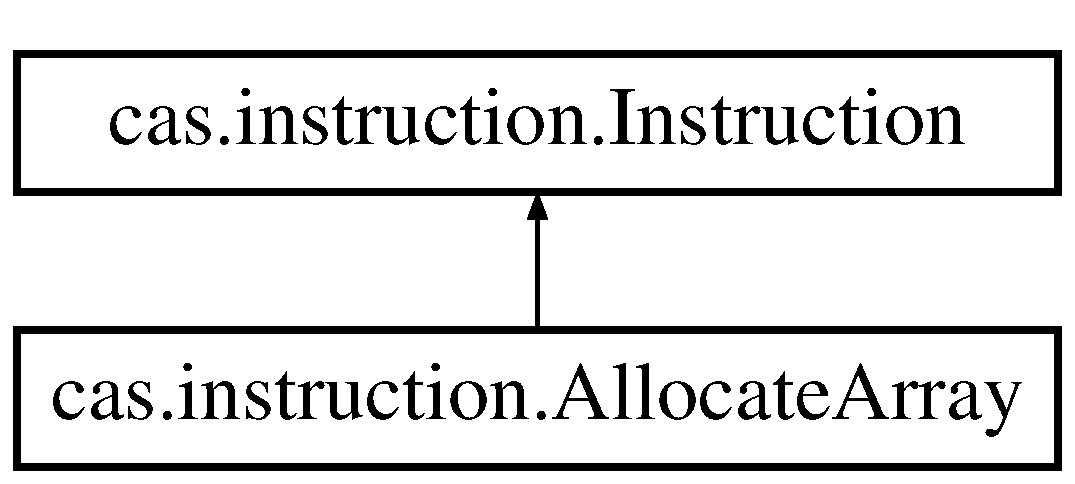
\includegraphics[height=2.000000cm]{classcas_1_1instruction_1_1_allocate_array}
\end{center}
\end{figure}
\subsection*{Public Member Functions}
\begin{DoxyCompactItemize}
\item 
\hyperlink{classcas_1_1instruction_1_1_allocate_array_a0df63de75ffdfe7c4097ff0667b63ea9}{Allocate\-Array} ()
\item 
\hyperlink{classcas_1_1instruction_1_1_allocate_array_a7acc69b0c436ad1005ed28cd5423ec29}{Allocate\-Array} (int location, int size\-Register)
\item 
int \hyperlink{classcas_1_1instruction_1_1_allocate_array_a607355f28f37787c87bb8799a48060b6}{size\-Register} ()
\item 
int \hyperlink{classcas_1_1instruction_1_1_allocate_array_afd6ab3ceecf895ee7548dc2c1a4a3787}{location} ()
\item 
void \hyperlink{classcas_1_1instruction_1_1_allocate_array_ad91621f2e7f4a9f062b9533986ff8019}{set\-Location} (int index)
\item 
void \hyperlink{classcas_1_1instruction_1_1_allocate_array_ad1d595b04d7f79c5be48a5f87cdd746b}{set\-Size\-Register} (int size\-Register)
\item 
String \hyperlink{classcas_1_1instruction_1_1_allocate_array_a7793a78d23230af92e5d996a6d63ee33}{to\-String} ()
\end{DoxyCompactItemize}


\subsection{Constructor \& Destructor Documentation}
\hypertarget{classcas_1_1instruction_1_1_allocate_array_a0df63de75ffdfe7c4097ff0667b63ea9}{\index{cas\-::instruction\-::\-Allocate\-Array@{cas\-::instruction\-::\-Allocate\-Array}!Allocate\-Array@{Allocate\-Array}}
\index{Allocate\-Array@{Allocate\-Array}!cas::instruction::AllocateArray@{cas\-::instruction\-::\-Allocate\-Array}}
\subsubsection[{Allocate\-Array}]{\setlength{\rightskip}{0pt plus 5cm}cas.\-instruction.\-Allocate\-Array.\-Allocate\-Array (
\begin{DoxyParamCaption}
{}
\end{DoxyParamCaption}
)}}\label{classcas_1_1instruction_1_1_allocate_array_a0df63de75ffdfe7c4097ff0667b63ea9}
\hypertarget{classcas_1_1instruction_1_1_allocate_array_a7acc69b0c436ad1005ed28cd5423ec29}{\index{cas\-::instruction\-::\-Allocate\-Array@{cas\-::instruction\-::\-Allocate\-Array}!Allocate\-Array@{Allocate\-Array}}
\index{Allocate\-Array@{Allocate\-Array}!cas::instruction::AllocateArray@{cas\-::instruction\-::\-Allocate\-Array}}
\subsubsection[{Allocate\-Array}]{\setlength{\rightskip}{0pt plus 5cm}cas.\-instruction.\-Allocate\-Array.\-Allocate\-Array (
\begin{DoxyParamCaption}
\item[{int}]{location, }
\item[{int}]{size\-Register}
\end{DoxyParamCaption}
)}}\label{classcas_1_1instruction_1_1_allocate_array_a7acc69b0c436ad1005ed28cd5423ec29}


\subsection{Member Function Documentation}
\hypertarget{classcas_1_1instruction_1_1_allocate_array_afd6ab3ceecf895ee7548dc2c1a4a3787}{\index{cas\-::instruction\-::\-Allocate\-Array@{cas\-::instruction\-::\-Allocate\-Array}!location@{location}}
\index{location@{location}!cas::instruction::AllocateArray@{cas\-::instruction\-::\-Allocate\-Array}}
\subsubsection[{location}]{\setlength{\rightskip}{0pt plus 5cm}int cas.\-instruction.\-Allocate\-Array.\-location (
\begin{DoxyParamCaption}
{}
\end{DoxyParamCaption}
)}}\label{classcas_1_1instruction_1_1_allocate_array_afd6ab3ceecf895ee7548dc2c1a4a3787}
\hypertarget{classcas_1_1instruction_1_1_allocate_array_ad91621f2e7f4a9f062b9533986ff8019}{\index{cas\-::instruction\-::\-Allocate\-Array@{cas\-::instruction\-::\-Allocate\-Array}!set\-Location@{set\-Location}}
\index{set\-Location@{set\-Location}!cas::instruction::AllocateArray@{cas\-::instruction\-::\-Allocate\-Array}}
\subsubsection[{set\-Location}]{\setlength{\rightskip}{0pt plus 5cm}void cas.\-instruction.\-Allocate\-Array.\-set\-Location (
\begin{DoxyParamCaption}
\item[{int}]{index}
\end{DoxyParamCaption}
)}}\label{classcas_1_1instruction_1_1_allocate_array_ad91621f2e7f4a9f062b9533986ff8019}
\hypertarget{classcas_1_1instruction_1_1_allocate_array_ad1d595b04d7f79c5be48a5f87cdd746b}{\index{cas\-::instruction\-::\-Allocate\-Array@{cas\-::instruction\-::\-Allocate\-Array}!set\-Size\-Register@{set\-Size\-Register}}
\index{set\-Size\-Register@{set\-Size\-Register}!cas::instruction::AllocateArray@{cas\-::instruction\-::\-Allocate\-Array}}
\subsubsection[{set\-Size\-Register}]{\setlength{\rightskip}{0pt plus 5cm}void cas.\-instruction.\-Allocate\-Array.\-set\-Size\-Register (
\begin{DoxyParamCaption}
\item[{int}]{size\-Register}
\end{DoxyParamCaption}
)}}\label{classcas_1_1instruction_1_1_allocate_array_ad1d595b04d7f79c5be48a5f87cdd746b}
\hypertarget{classcas_1_1instruction_1_1_allocate_array_a607355f28f37787c87bb8799a48060b6}{\index{cas\-::instruction\-::\-Allocate\-Array@{cas\-::instruction\-::\-Allocate\-Array}!size\-Register@{size\-Register}}
\index{size\-Register@{size\-Register}!cas::instruction::AllocateArray@{cas\-::instruction\-::\-Allocate\-Array}}
\subsubsection[{size\-Register}]{\setlength{\rightskip}{0pt plus 5cm}int cas.\-instruction.\-Allocate\-Array.\-size\-Register (
\begin{DoxyParamCaption}
{}
\end{DoxyParamCaption}
)}}\label{classcas_1_1instruction_1_1_allocate_array_a607355f28f37787c87bb8799a48060b6}
\hypertarget{classcas_1_1instruction_1_1_allocate_array_a7793a78d23230af92e5d996a6d63ee33}{\index{cas\-::instruction\-::\-Allocate\-Array@{cas\-::instruction\-::\-Allocate\-Array}!to\-String@{to\-String}}
\index{to\-String@{to\-String}!cas::instruction::AllocateArray@{cas\-::instruction\-::\-Allocate\-Array}}
\subsubsection[{to\-String}]{\setlength{\rightskip}{0pt plus 5cm}String cas.\-instruction.\-Allocate\-Array.\-to\-String (
\begin{DoxyParamCaption}
{}
\end{DoxyParamCaption}
)\hspace{0.3cm}{\ttfamily [virtual]}}}\label{classcas_1_1instruction_1_1_allocate_array_a7793a78d23230af92e5d996a6d63ee33}


Implements \hyperlink{classcas_1_1instruction_1_1_instruction_a7992edd8d79e1a4e82fb44f4c9abacf9}{cas.\-instruction.\-Instruction}.



The documentation for this class was generated from the following file\-:\begin{DoxyCompactItemize}
\item 
cas/instruction/\hyperlink{_allocate_array_8java}{Allocate\-Array.\-java}\end{DoxyCompactItemize}

\hypertarget{classcas_1_1automata_1_1_automata}{\section{cas.\-automata.\-Automata Class Reference}
\label{classcas_1_1automata_1_1_automata}\index{cas.\-automata.\-Automata@{cas.\-automata.\-Automata}}
}
\subsection*{Public Member Functions}
\begin{DoxyCompactItemize}
\item 
\hyperlink{classcas_1_1automata_1_1_automata_a167be64ae393f0acccede8b34eb2fe01}{Automata} (int edge\-Size, int dimension, int radius, int states, \hyperlink{classcas_1_1machine_1_1_virtual_machine}{Virtual\-Machine} virtual\-Machine)
\item 
void \hyperlink{classcas_1_1automata_1_1_automata_ac0c8bfa08108b7c395c0acc22524ee43}{build\-Neigborhood\-Coordinates} ()
\item 
Integer\mbox{[}$\,$\mbox{]} \hyperlink{classcas_1_1automata_1_1_automata_a25246d39284f98b88886e07b909ad2b1}{get\-Neigborhood} (int index)
\item 
int \hyperlink{classcas_1_1automata_1_1_automata_ad6356ae105168abc3d974a4f2d7f8884}{update\-Neigborhood} (Integer\mbox{[}$\,$\mbox{]} update\-Neighborhood)
\item 
void \hyperlink{classcas_1_1automata_1_1_automata_a719d3b4a9839a3f2cb5abc3aefeb60a1}{update} ()
\item 
void \hyperlink{classcas_1_1automata_1_1_automata_ac4f921807b4ee47bbd6d239548e0ffbc}{update} (int steps)
\item 
void \hyperlink{classcas_1_1automata_1_1_automata_a69420deb2c5cc45bc931862683642661}{set\-Cell} (int index, int state)
\item 
void \hyperlink{classcas_1_1automata_1_1_automata_ab44636a24ef1719759e27af66616d9b7}{generate\-Random\-Configuration} ()
\item 
String \hyperlink{classcas_1_1automata_1_1_automata_aaf6d92da07939b9881bba66f4cbfdabb}{to\-String} ()
\item 
void \hyperlink{classcas_1_1automata_1_1_automata_a5505d33bee6fe4a0ca848905a5a4db1e}{set\-Configuration} (int\mbox{[}$\,$\mbox{]} configuration)
\item 
int \hyperlink{classcas_1_1automata_1_1_automata_ab8d1f9f13ddfd86150086234820f1eb2}{get\-Size} ()
\item 
int \hyperlink{classcas_1_1automata_1_1_automata_a16d4ff448a380de7dd768bb0ce8961e8}{get\-Number\-Cells} ()
\item 
int \hyperlink{classcas_1_1automata_1_1_automata_a3e9638dbc5d7897106246cac441fb82b}{get\-Dimension} ()
\item 
int \hyperlink{classcas_1_1automata_1_1_automata_a6fbee4c818b5a5391c538fe7d8a4c2a9}{get\-States} ()
\item 
int\mbox{[}$\,$\mbox{]} \hyperlink{classcas_1_1automata_1_1_automata_a64fd03e09e2f98579032360debcbd456}{get\-Cell\-Space} ()
\end{DoxyCompactItemize}


\subsection{Constructor \& Destructor Documentation}
\hypertarget{classcas_1_1automata_1_1_automata_a167be64ae393f0acccede8b34eb2fe01}{\index{cas\-::automata\-::\-Automata@{cas\-::automata\-::\-Automata}!Automata@{Automata}}
\index{Automata@{Automata}!cas::automata::Automata@{cas\-::automata\-::\-Automata}}
\subsubsection[{Automata}]{\setlength{\rightskip}{0pt plus 5cm}cas.\-automata.\-Automata.\-Automata (
\begin{DoxyParamCaption}
\item[{int}]{edge\-Size, }
\item[{int}]{dimension, }
\item[{int}]{radius, }
\item[{int}]{states, }
\item[{{\bf Virtual\-Machine}}]{virtual\-Machine}
\end{DoxyParamCaption}
)}}\label{classcas_1_1automata_1_1_automata_a167be64ae393f0acccede8b34eb2fe01}


\subsection{Member Function Documentation}
\hypertarget{classcas_1_1automata_1_1_automata_ac0c8bfa08108b7c395c0acc22524ee43}{\index{cas\-::automata\-::\-Automata@{cas\-::automata\-::\-Automata}!build\-Neigborhood\-Coordinates@{build\-Neigborhood\-Coordinates}}
\index{build\-Neigborhood\-Coordinates@{build\-Neigborhood\-Coordinates}!cas::automata::Automata@{cas\-::automata\-::\-Automata}}
\subsubsection[{build\-Neigborhood\-Coordinates}]{\setlength{\rightskip}{0pt plus 5cm}void cas.\-automata.\-Automata.\-build\-Neigborhood\-Coordinates (
\begin{DoxyParamCaption}
{}
\end{DoxyParamCaption}
)}}\label{classcas_1_1automata_1_1_automata_ac0c8bfa08108b7c395c0acc22524ee43}
\hypertarget{classcas_1_1automata_1_1_automata_ab44636a24ef1719759e27af66616d9b7}{\index{cas\-::automata\-::\-Automata@{cas\-::automata\-::\-Automata}!generate\-Random\-Configuration@{generate\-Random\-Configuration}}
\index{generate\-Random\-Configuration@{generate\-Random\-Configuration}!cas::automata::Automata@{cas\-::automata\-::\-Automata}}
\subsubsection[{generate\-Random\-Configuration}]{\setlength{\rightskip}{0pt plus 5cm}void cas.\-automata.\-Automata.\-generate\-Random\-Configuration (
\begin{DoxyParamCaption}
{}
\end{DoxyParamCaption}
)}}\label{classcas_1_1automata_1_1_automata_ab44636a24ef1719759e27af66616d9b7}
\hypertarget{classcas_1_1automata_1_1_automata_a64fd03e09e2f98579032360debcbd456}{\index{cas\-::automata\-::\-Automata@{cas\-::automata\-::\-Automata}!get\-Cell\-Space@{get\-Cell\-Space}}
\index{get\-Cell\-Space@{get\-Cell\-Space}!cas::automata::Automata@{cas\-::automata\-::\-Automata}}
\subsubsection[{get\-Cell\-Space}]{\setlength{\rightskip}{0pt plus 5cm}int \mbox{[}$\,$\mbox{]} cas.\-automata.\-Automata.\-get\-Cell\-Space (
\begin{DoxyParamCaption}
{}
\end{DoxyParamCaption}
)}}\label{classcas_1_1automata_1_1_automata_a64fd03e09e2f98579032360debcbd456}
\hypertarget{classcas_1_1automata_1_1_automata_a3e9638dbc5d7897106246cac441fb82b}{\index{cas\-::automata\-::\-Automata@{cas\-::automata\-::\-Automata}!get\-Dimension@{get\-Dimension}}
\index{get\-Dimension@{get\-Dimension}!cas::automata::Automata@{cas\-::automata\-::\-Automata}}
\subsubsection[{get\-Dimension}]{\setlength{\rightskip}{0pt plus 5cm}int cas.\-automata.\-Automata.\-get\-Dimension (
\begin{DoxyParamCaption}
{}
\end{DoxyParamCaption}
)}}\label{classcas_1_1automata_1_1_automata_a3e9638dbc5d7897106246cac441fb82b}
\hypertarget{classcas_1_1automata_1_1_automata_a25246d39284f98b88886e07b909ad2b1}{\index{cas\-::automata\-::\-Automata@{cas\-::automata\-::\-Automata}!get\-Neigborhood@{get\-Neigborhood}}
\index{get\-Neigborhood@{get\-Neigborhood}!cas::automata::Automata@{cas\-::automata\-::\-Automata}}
\subsubsection[{get\-Neigborhood}]{\setlength{\rightskip}{0pt plus 5cm}Integer \mbox{[}$\,$\mbox{]} cas.\-automata.\-Automata.\-get\-Neigborhood (
\begin{DoxyParamCaption}
\item[{int}]{index}
\end{DoxyParamCaption}
)}}\label{classcas_1_1automata_1_1_automata_a25246d39284f98b88886e07b909ad2b1}
\hypertarget{classcas_1_1automata_1_1_automata_a16d4ff448a380de7dd768bb0ce8961e8}{\index{cas\-::automata\-::\-Automata@{cas\-::automata\-::\-Automata}!get\-Number\-Cells@{get\-Number\-Cells}}
\index{get\-Number\-Cells@{get\-Number\-Cells}!cas::automata::Automata@{cas\-::automata\-::\-Automata}}
\subsubsection[{get\-Number\-Cells}]{\setlength{\rightskip}{0pt plus 5cm}int cas.\-automata.\-Automata.\-get\-Number\-Cells (
\begin{DoxyParamCaption}
{}
\end{DoxyParamCaption}
)}}\label{classcas_1_1automata_1_1_automata_a16d4ff448a380de7dd768bb0ce8961e8}
\hypertarget{classcas_1_1automata_1_1_automata_ab8d1f9f13ddfd86150086234820f1eb2}{\index{cas\-::automata\-::\-Automata@{cas\-::automata\-::\-Automata}!get\-Size@{get\-Size}}
\index{get\-Size@{get\-Size}!cas::automata::Automata@{cas\-::automata\-::\-Automata}}
\subsubsection[{get\-Size}]{\setlength{\rightskip}{0pt plus 5cm}int cas.\-automata.\-Automata.\-get\-Size (
\begin{DoxyParamCaption}
{}
\end{DoxyParamCaption}
)}}\label{classcas_1_1automata_1_1_automata_ab8d1f9f13ddfd86150086234820f1eb2}
\hypertarget{classcas_1_1automata_1_1_automata_a6fbee4c818b5a5391c538fe7d8a4c2a9}{\index{cas\-::automata\-::\-Automata@{cas\-::automata\-::\-Automata}!get\-States@{get\-States}}
\index{get\-States@{get\-States}!cas::automata::Automata@{cas\-::automata\-::\-Automata}}
\subsubsection[{get\-States}]{\setlength{\rightskip}{0pt plus 5cm}int cas.\-automata.\-Automata.\-get\-States (
\begin{DoxyParamCaption}
{}
\end{DoxyParamCaption}
)}}\label{classcas_1_1automata_1_1_automata_a6fbee4c818b5a5391c538fe7d8a4c2a9}
\hypertarget{classcas_1_1automata_1_1_automata_a69420deb2c5cc45bc931862683642661}{\index{cas\-::automata\-::\-Automata@{cas\-::automata\-::\-Automata}!set\-Cell@{set\-Cell}}
\index{set\-Cell@{set\-Cell}!cas::automata::Automata@{cas\-::automata\-::\-Automata}}
\subsubsection[{set\-Cell}]{\setlength{\rightskip}{0pt plus 5cm}void cas.\-automata.\-Automata.\-set\-Cell (
\begin{DoxyParamCaption}
\item[{int}]{index, }
\item[{int}]{state}
\end{DoxyParamCaption}
)}}\label{classcas_1_1automata_1_1_automata_a69420deb2c5cc45bc931862683642661}
\hypertarget{classcas_1_1automata_1_1_automata_a5505d33bee6fe4a0ca848905a5a4db1e}{\index{cas\-::automata\-::\-Automata@{cas\-::automata\-::\-Automata}!set\-Configuration@{set\-Configuration}}
\index{set\-Configuration@{set\-Configuration}!cas::automata::Automata@{cas\-::automata\-::\-Automata}}
\subsubsection[{set\-Configuration}]{\setlength{\rightskip}{0pt plus 5cm}void cas.\-automata.\-Automata.\-set\-Configuration (
\begin{DoxyParamCaption}
\item[{int\mbox{[}$\,$\mbox{]}}]{configuration}
\end{DoxyParamCaption}
)}}\label{classcas_1_1automata_1_1_automata_a5505d33bee6fe4a0ca848905a5a4db1e}
\hypertarget{classcas_1_1automata_1_1_automata_aaf6d92da07939b9881bba66f4cbfdabb}{\index{cas\-::automata\-::\-Automata@{cas\-::automata\-::\-Automata}!to\-String@{to\-String}}
\index{to\-String@{to\-String}!cas::automata::Automata@{cas\-::automata\-::\-Automata}}
\subsubsection[{to\-String}]{\setlength{\rightskip}{0pt plus 5cm}String cas.\-automata.\-Automata.\-to\-String (
\begin{DoxyParamCaption}
{}
\end{DoxyParamCaption}
)}}\label{classcas_1_1automata_1_1_automata_aaf6d92da07939b9881bba66f4cbfdabb}
\hypertarget{classcas_1_1automata_1_1_automata_a719d3b4a9839a3f2cb5abc3aefeb60a1}{\index{cas\-::automata\-::\-Automata@{cas\-::automata\-::\-Automata}!update@{update}}
\index{update@{update}!cas::automata::Automata@{cas\-::automata\-::\-Automata}}
\subsubsection[{update}]{\setlength{\rightskip}{0pt plus 5cm}void cas.\-automata.\-Automata.\-update (
\begin{DoxyParamCaption}
{}
\end{DoxyParamCaption}
)}}\label{classcas_1_1automata_1_1_automata_a719d3b4a9839a3f2cb5abc3aefeb60a1}
\hypertarget{classcas_1_1automata_1_1_automata_ac4f921807b4ee47bbd6d239548e0ffbc}{\index{cas\-::automata\-::\-Automata@{cas\-::automata\-::\-Automata}!update@{update}}
\index{update@{update}!cas::automata::Automata@{cas\-::automata\-::\-Automata}}
\subsubsection[{update}]{\setlength{\rightskip}{0pt plus 5cm}void cas.\-automata.\-Automata.\-update (
\begin{DoxyParamCaption}
\item[{int}]{steps}
\end{DoxyParamCaption}
)}}\label{classcas_1_1automata_1_1_automata_ac4f921807b4ee47bbd6d239548e0ffbc}
\hypertarget{classcas_1_1automata_1_1_automata_ad6356ae105168abc3d974a4f2d7f8884}{\index{cas\-::automata\-::\-Automata@{cas\-::automata\-::\-Automata}!update\-Neigborhood@{update\-Neigborhood}}
\index{update\-Neigborhood@{update\-Neigborhood}!cas::automata::Automata@{cas\-::automata\-::\-Automata}}
\subsubsection[{update\-Neigborhood}]{\setlength{\rightskip}{0pt plus 5cm}int cas.\-automata.\-Automata.\-update\-Neigborhood (
\begin{DoxyParamCaption}
\item[{Integer\mbox{[}$\,$\mbox{]}}]{update\-Neighborhood}
\end{DoxyParamCaption}
)}}\label{classcas_1_1automata_1_1_automata_ad6356ae105168abc3d974a4f2d7f8884}


The documentation for this class was generated from the following file\-:\begin{DoxyCompactItemize}
\item 
cas/automata/\hyperlink{_automata_8java}{Automata.\-java}\end{DoxyCompactItemize}

\hypertarget{classcas_1_1instruction_1_1_break}{\section{cas.\-instruction.\-Break Class Reference}
\label{classcas_1_1instruction_1_1_break}\index{cas.\-instruction.\-Break@{cas.\-instruction.\-Break}}
}
Inheritance diagram for cas.\-instruction.\-Break\-:\begin{figure}[H]
\begin{center}
\leavevmode
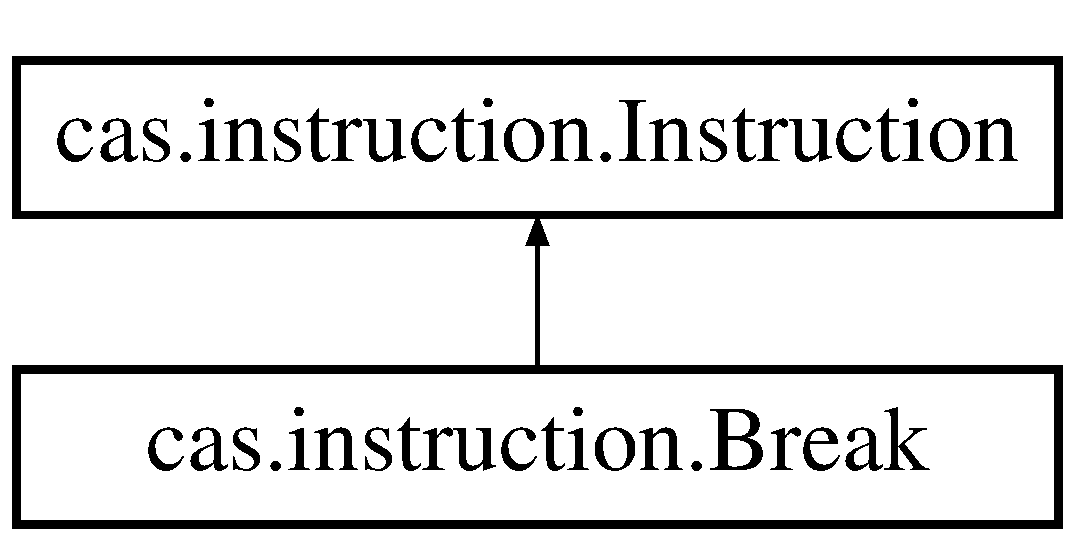
\includegraphics[height=2.000000cm]{classcas_1_1instruction_1_1_break}
\end{center}
\end{figure}
\subsection*{Classes}
\begin{DoxyCompactItemize}
\item 
enum \hyperlink{enumcas_1_1instruction_1_1_break_1_1_condition}{Condition}
\end{DoxyCompactItemize}
\subsection*{Public Member Functions}
\begin{DoxyCompactItemize}
\item 
\hyperlink{classcas_1_1instruction_1_1_break_a8bb03ff69ea5fcdb6ca65592a83bba7a}{Break} ()
\item 
\hyperlink{classcas_1_1instruction_1_1_break_a46af18ace0ccff16766c9e2d0125d50f}{Break} (\hyperlink{enumcas_1_1instruction_1_1_break_1_1_condition}{Condition} condition, int source\-Reg, int jump\-To)
\item 
\hyperlink{enumcas_1_1instruction_1_1_break_1_1_condition}{Condition} \hyperlink{classcas_1_1instruction_1_1_break_a9f8f8d465c12b17f10d2563a7ed5f3ff}{get\-Condition} ()
\item 
int \hyperlink{classcas_1_1instruction_1_1_break_ae7304e16507fc9365a3e6d0bfe224b1b}{get\-Source} ()
\item 
int \hyperlink{classcas_1_1instruction_1_1_break_a3be3ac780c73fd9a31e7cc740f40b475}{get\-Offset} ()
\item 
String \hyperlink{classcas_1_1instruction_1_1_break_a3403130e65dafa6b1db3e7524836e6ae}{to\-String} ()
\item 
void \hyperlink{classcas_1_1instruction_1_1_break_ad25ef55cc8c7c6cc5776cd08cf6b0e78}{set\-Condition} (\hyperlink{enumcas_1_1instruction_1_1_break_1_1_condition}{Condition} condition)
\item 
void \hyperlink{classcas_1_1instruction_1_1_break_ac7311832c23abf2dc3e881b78803291c}{set\-Jump\-Index} (int offset)
\item 
void \hyperlink{classcas_1_1instruction_1_1_break_aadc3c672af83c33bdf50bcdbbb22b8a7}{set\-Souce} (int register)
\end{DoxyCompactItemize}


\subsection{Constructor \& Destructor Documentation}
\hypertarget{classcas_1_1instruction_1_1_break_a8bb03ff69ea5fcdb6ca65592a83bba7a}{\index{cas\-::instruction\-::\-Break@{cas\-::instruction\-::\-Break}!Break@{Break}}
\index{Break@{Break}!cas::instruction::Break@{cas\-::instruction\-::\-Break}}
\subsubsection[{Break}]{\setlength{\rightskip}{0pt plus 5cm}cas.\-instruction.\-Break.\-Break (
\begin{DoxyParamCaption}
{}
\end{DoxyParamCaption}
)}}\label{classcas_1_1instruction_1_1_break_a8bb03ff69ea5fcdb6ca65592a83bba7a}
\hypertarget{classcas_1_1instruction_1_1_break_a46af18ace0ccff16766c9e2d0125d50f}{\index{cas\-::instruction\-::\-Break@{cas\-::instruction\-::\-Break}!Break@{Break}}
\index{Break@{Break}!cas::instruction::Break@{cas\-::instruction\-::\-Break}}
\subsubsection[{Break}]{\setlength{\rightskip}{0pt plus 5cm}cas.\-instruction.\-Break.\-Break (
\begin{DoxyParamCaption}
\item[{{\bf Condition}}]{condition, }
\item[{int}]{source\-Reg, }
\item[{int}]{jump\-To}
\end{DoxyParamCaption}
)}}\label{classcas_1_1instruction_1_1_break_a46af18ace0ccff16766c9e2d0125d50f}


\subsection{Member Function Documentation}
\hypertarget{classcas_1_1instruction_1_1_break_a9f8f8d465c12b17f10d2563a7ed5f3ff}{\index{cas\-::instruction\-::\-Break@{cas\-::instruction\-::\-Break}!get\-Condition@{get\-Condition}}
\index{get\-Condition@{get\-Condition}!cas::instruction::Break@{cas\-::instruction\-::\-Break}}
\subsubsection[{get\-Condition}]{\setlength{\rightskip}{0pt plus 5cm}{\bf Condition} cas.\-instruction.\-Break.\-get\-Condition (
\begin{DoxyParamCaption}
{}
\end{DoxyParamCaption}
)}}\label{classcas_1_1instruction_1_1_break_a9f8f8d465c12b17f10d2563a7ed5f3ff}
\hypertarget{classcas_1_1instruction_1_1_break_a3be3ac780c73fd9a31e7cc740f40b475}{\index{cas\-::instruction\-::\-Break@{cas\-::instruction\-::\-Break}!get\-Offset@{get\-Offset}}
\index{get\-Offset@{get\-Offset}!cas::instruction::Break@{cas\-::instruction\-::\-Break}}
\subsubsection[{get\-Offset}]{\setlength{\rightskip}{0pt plus 5cm}int cas.\-instruction.\-Break.\-get\-Offset (
\begin{DoxyParamCaption}
{}
\end{DoxyParamCaption}
)}}\label{classcas_1_1instruction_1_1_break_a3be3ac780c73fd9a31e7cc740f40b475}
\hypertarget{classcas_1_1instruction_1_1_break_ae7304e16507fc9365a3e6d0bfe224b1b}{\index{cas\-::instruction\-::\-Break@{cas\-::instruction\-::\-Break}!get\-Source@{get\-Source}}
\index{get\-Source@{get\-Source}!cas::instruction::Break@{cas\-::instruction\-::\-Break}}
\subsubsection[{get\-Source}]{\setlength{\rightskip}{0pt plus 5cm}int cas.\-instruction.\-Break.\-get\-Source (
\begin{DoxyParamCaption}
{}
\end{DoxyParamCaption}
)}}\label{classcas_1_1instruction_1_1_break_ae7304e16507fc9365a3e6d0bfe224b1b}
\hypertarget{classcas_1_1instruction_1_1_break_ad25ef55cc8c7c6cc5776cd08cf6b0e78}{\index{cas\-::instruction\-::\-Break@{cas\-::instruction\-::\-Break}!set\-Condition@{set\-Condition}}
\index{set\-Condition@{set\-Condition}!cas::instruction::Break@{cas\-::instruction\-::\-Break}}
\subsubsection[{set\-Condition}]{\setlength{\rightskip}{0pt plus 5cm}void cas.\-instruction.\-Break.\-set\-Condition (
\begin{DoxyParamCaption}
\item[{{\bf Condition}}]{condition}
\end{DoxyParamCaption}
)}}\label{classcas_1_1instruction_1_1_break_ad25ef55cc8c7c6cc5776cd08cf6b0e78}
\hypertarget{classcas_1_1instruction_1_1_break_ac7311832c23abf2dc3e881b78803291c}{\index{cas\-::instruction\-::\-Break@{cas\-::instruction\-::\-Break}!set\-Jump\-Index@{set\-Jump\-Index}}
\index{set\-Jump\-Index@{set\-Jump\-Index}!cas::instruction::Break@{cas\-::instruction\-::\-Break}}
\subsubsection[{set\-Jump\-Index}]{\setlength{\rightskip}{0pt plus 5cm}void cas.\-instruction.\-Break.\-set\-Jump\-Index (
\begin{DoxyParamCaption}
\item[{int}]{offset}
\end{DoxyParamCaption}
)}}\label{classcas_1_1instruction_1_1_break_ac7311832c23abf2dc3e881b78803291c}
\hypertarget{classcas_1_1instruction_1_1_break_aadc3c672af83c33bdf50bcdbbb22b8a7}{\index{cas\-::instruction\-::\-Break@{cas\-::instruction\-::\-Break}!set\-Souce@{set\-Souce}}
\index{set\-Souce@{set\-Souce}!cas::instruction::Break@{cas\-::instruction\-::\-Break}}
\subsubsection[{set\-Souce}]{\setlength{\rightskip}{0pt plus 5cm}void cas.\-instruction.\-Break.\-set\-Souce (
\begin{DoxyParamCaption}
\item[{int}]{register}
\end{DoxyParamCaption}
)}}\label{classcas_1_1instruction_1_1_break_aadc3c672af83c33bdf50bcdbbb22b8a7}
\hypertarget{classcas_1_1instruction_1_1_break_a3403130e65dafa6b1db3e7524836e6ae}{\index{cas\-::instruction\-::\-Break@{cas\-::instruction\-::\-Break}!to\-String@{to\-String}}
\index{to\-String@{to\-String}!cas::instruction::Break@{cas\-::instruction\-::\-Break}}
\subsubsection[{to\-String}]{\setlength{\rightskip}{0pt plus 5cm}String cas.\-instruction.\-Break.\-to\-String (
\begin{DoxyParamCaption}
{}
\end{DoxyParamCaption}
)\hspace{0.3cm}{\ttfamily [virtual]}}}\label{classcas_1_1instruction_1_1_break_a3403130e65dafa6b1db3e7524836e6ae}


Implements \hyperlink{classcas_1_1instruction_1_1_instruction_a7992edd8d79e1a4e82fb44f4c9abacf9}{cas.\-instruction.\-Instruction}.



The documentation for this class was generated from the following file\-:\begin{DoxyCompactItemize}
\item 
cas/instruction/\hyperlink{_break_8java}{Break.\-java}\end{DoxyCompactItemize}

\hypertarget{classcas_1_1parser_1_1parser__containers_1_1_code_list}{\section{cas.\-parser.\-parser\-\_\-containers.\-Code\-List Class Reference}
\label{classcas_1_1parser_1_1parser__containers_1_1_code_list}\index{cas.\-parser.\-parser\-\_\-containers.\-Code\-List@{cas.\-parser.\-parser\-\_\-containers.\-Code\-List}}
}
Inheritance diagram for cas.\-parser.\-parser\-\_\-containers.\-Code\-List\-:\begin{figure}[H]
\begin{center}
\leavevmode
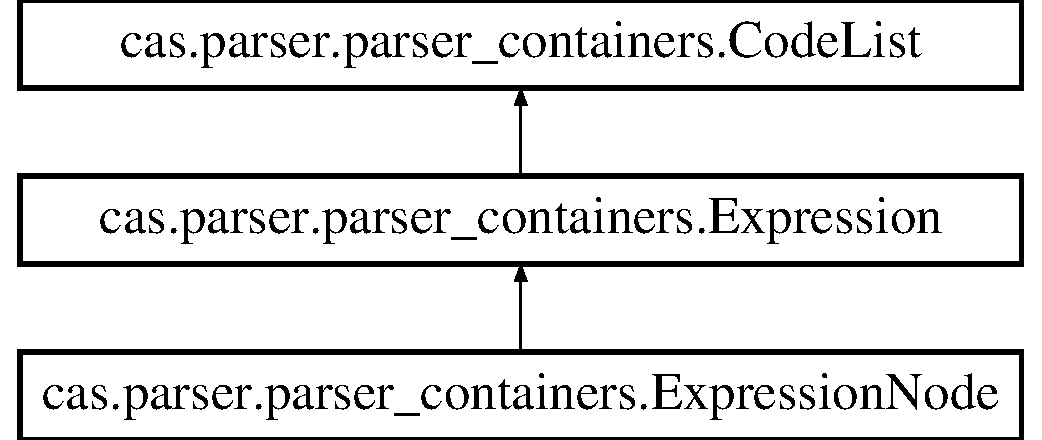
\includegraphics[height=3.000000cm]{classcas_1_1parser_1_1parser__containers_1_1_code_list}
\end{center}
\end{figure}
\subsection*{Public Member Functions}
\begin{DoxyCompactItemize}
\item 
\hyperlink{classcas_1_1parser_1_1parser__containers_1_1_code_list_a6ddc761881342b6ec9ed3e202eb9e13c}{Code\-List} ()
\item 
\hyperlink{classcas_1_1parser_1_1parser__containers_1_1_code_list_a71addf91d1c62a09e8838f50bdd28f6f}{Code\-List} (\hyperlink{classcas_1_1parser_1_1parser__containers_1_1_code_list}{Code\-List} other\-List)
\item 
\hyperlink{classcas_1_1parser_1_1parser__containers_1_1_code_list_a1ad0745dfaea07e2f9ca1160e8f11852}{Code\-List} (Array\-List$<$ \hyperlink{classcas_1_1instruction_1_1_instruction}{Instruction} $>$ instruction\-Array)
\item 
Array\-List$<$ \hyperlink{classcas_1_1instruction_1_1_instruction}{Instruction} $>$ \hyperlink{classcas_1_1parser_1_1parser__containers_1_1_code_list_ae8e046c8a8c9d2c494b4b3ae73255181}{get\-Instruction\-List} ()
\item 
\hyperlink{classcas_1_1instruction_1_1_instruction}{Instruction}\mbox{[}$\,$\mbox{]} \hyperlink{classcas_1_1parser_1_1parser__containers_1_1_code_list_a6d2ad7bcdb310e57ad7015fec8a31b18}{to\-Array} ()
\item 
\hyperlink{classcas_1_1instruction_1_1_instruction}{Instruction} \hyperlink{classcas_1_1parser_1_1parser__containers_1_1_code_list_af4112f3cfa8351a163f2d3beca017085}{get} (int index)
\item 
int \hyperlink{classcas_1_1parser_1_1parser__containers_1_1_code_list_ac62b7f02ab81c23688c1dbc4c13ec79b}{size} ()
\item 
void \hyperlink{classcas_1_1parser_1_1parser__containers_1_1_code_list_a8b8f38668a8e672c0ddf93c841380d68}{append} (\hyperlink{classcas_1_1instruction_1_1_instruction}{Instruction} instruction)
\item 
void \hyperlink{classcas_1_1parser_1_1parser__containers_1_1_code_list_a737e0eb573359698781fbf528bcccd54}{append} (Array\-List$<$ \hyperlink{classcas_1_1instruction_1_1_instruction}{Instruction} $>$ instructions)
\item 
void \hyperlink{classcas_1_1parser_1_1parser__containers_1_1_code_list_ac6c07c1c4c3fc025ec598f6bb60cdfdf}{append} (\hyperlink{classcas_1_1parser_1_1parser__containers_1_1_code_list}{Code\-List} list)
\item 
void \hyperlink{classcas_1_1parser_1_1parser__containers_1_1_code_list_aa9cf24f683ecf4c7dda2c70581f9a502}{prepend} (\hyperlink{classcas_1_1instruction_1_1_instruction}{Instruction} instruction)
\item 
void \hyperlink{classcas_1_1parser_1_1parser__containers_1_1_code_list_a1f72f45876ccba2fef50a3c83e2b1f0c}{prepend} (Array\-List$<$ \hyperlink{classcas_1_1instruction_1_1_instruction}{Instruction} $>$ instructions)
\item 
void \hyperlink{classcas_1_1parser_1_1parser__containers_1_1_code_list_af0055068ffe6784b0ed4c26d2c5b28b7}{set\-Instructions} (Array\-List$<$ \hyperlink{classcas_1_1instruction_1_1_instruction}{Instruction} $>$ instructions)
\item 
void \hyperlink{classcas_1_1parser_1_1parser__containers_1_1_code_list_a596cb7a533ed8b2691463bb9cf80188c}{set} (int index, \hyperlink{classcas_1_1instruction_1_1_instruction}{Instruction} element)
\item 
String \hyperlink{classcas_1_1parser_1_1parser__containers_1_1_code_list_a9e5369166a1c95cc564cb0d5ee110906}{to\-String} ()
\end{DoxyCompactItemize}
\subsection*{Protected Attributes}
\begin{DoxyCompactItemize}
\item 
Array\-List$<$ \hyperlink{classcas_1_1instruction_1_1_instruction}{Instruction} $>$ \hyperlink{classcas_1_1parser_1_1parser__containers_1_1_code_list_a4a93e4fcdc23551521463643f0ecb1a3}{instruction\-List}
\end{DoxyCompactItemize}


\subsection{Constructor \& Destructor Documentation}
\hypertarget{classcas_1_1parser_1_1parser__containers_1_1_code_list_a6ddc761881342b6ec9ed3e202eb9e13c}{\index{cas\-::parser\-::parser\-\_\-containers\-::\-Code\-List@{cas\-::parser\-::parser\-\_\-containers\-::\-Code\-List}!Code\-List@{Code\-List}}
\index{Code\-List@{Code\-List}!cas::parser::parser_containers::CodeList@{cas\-::parser\-::parser\-\_\-containers\-::\-Code\-List}}
\subsubsection[{Code\-List}]{\setlength{\rightskip}{0pt plus 5cm}cas.\-parser.\-parser\-\_\-containers.\-Code\-List.\-Code\-List (
\begin{DoxyParamCaption}
{}
\end{DoxyParamCaption}
)}}\label{classcas_1_1parser_1_1parser__containers_1_1_code_list_a6ddc761881342b6ec9ed3e202eb9e13c}
\hypertarget{classcas_1_1parser_1_1parser__containers_1_1_code_list_a71addf91d1c62a09e8838f50bdd28f6f}{\index{cas\-::parser\-::parser\-\_\-containers\-::\-Code\-List@{cas\-::parser\-::parser\-\_\-containers\-::\-Code\-List}!Code\-List@{Code\-List}}
\index{Code\-List@{Code\-List}!cas::parser::parser_containers::CodeList@{cas\-::parser\-::parser\-\_\-containers\-::\-Code\-List}}
\subsubsection[{Code\-List}]{\setlength{\rightskip}{0pt plus 5cm}cas.\-parser.\-parser\-\_\-containers.\-Code\-List.\-Code\-List (
\begin{DoxyParamCaption}
\item[{{\bf Code\-List}}]{other\-List}
\end{DoxyParamCaption}
)}}\label{classcas_1_1parser_1_1parser__containers_1_1_code_list_a71addf91d1c62a09e8838f50bdd28f6f}
\hypertarget{classcas_1_1parser_1_1parser__containers_1_1_code_list_a1ad0745dfaea07e2f9ca1160e8f11852}{\index{cas\-::parser\-::parser\-\_\-containers\-::\-Code\-List@{cas\-::parser\-::parser\-\_\-containers\-::\-Code\-List}!Code\-List@{Code\-List}}
\index{Code\-List@{Code\-List}!cas::parser::parser_containers::CodeList@{cas\-::parser\-::parser\-\_\-containers\-::\-Code\-List}}
\subsubsection[{Code\-List}]{\setlength{\rightskip}{0pt plus 5cm}cas.\-parser.\-parser\-\_\-containers.\-Code\-List.\-Code\-List (
\begin{DoxyParamCaption}
\item[{Array\-List$<$ {\bf Instruction} $>$}]{instruction\-Array}
\end{DoxyParamCaption}
)}}\label{classcas_1_1parser_1_1parser__containers_1_1_code_list_a1ad0745dfaea07e2f9ca1160e8f11852}


\subsection{Member Function Documentation}
\hypertarget{classcas_1_1parser_1_1parser__containers_1_1_code_list_a8b8f38668a8e672c0ddf93c841380d68}{\index{cas\-::parser\-::parser\-\_\-containers\-::\-Code\-List@{cas\-::parser\-::parser\-\_\-containers\-::\-Code\-List}!append@{append}}
\index{append@{append}!cas::parser::parser_containers::CodeList@{cas\-::parser\-::parser\-\_\-containers\-::\-Code\-List}}
\subsubsection[{append}]{\setlength{\rightskip}{0pt plus 5cm}void cas.\-parser.\-parser\-\_\-containers.\-Code\-List.\-append (
\begin{DoxyParamCaption}
\item[{{\bf Instruction}}]{instruction}
\end{DoxyParamCaption}
)}}\label{classcas_1_1parser_1_1parser__containers_1_1_code_list_a8b8f38668a8e672c0ddf93c841380d68}
\hypertarget{classcas_1_1parser_1_1parser__containers_1_1_code_list_a737e0eb573359698781fbf528bcccd54}{\index{cas\-::parser\-::parser\-\_\-containers\-::\-Code\-List@{cas\-::parser\-::parser\-\_\-containers\-::\-Code\-List}!append@{append}}
\index{append@{append}!cas::parser::parser_containers::CodeList@{cas\-::parser\-::parser\-\_\-containers\-::\-Code\-List}}
\subsubsection[{append}]{\setlength{\rightskip}{0pt plus 5cm}void cas.\-parser.\-parser\-\_\-containers.\-Code\-List.\-append (
\begin{DoxyParamCaption}
\item[{Array\-List$<$ {\bf Instruction} $>$}]{instructions}
\end{DoxyParamCaption}
)}}\label{classcas_1_1parser_1_1parser__containers_1_1_code_list_a737e0eb573359698781fbf528bcccd54}
\hypertarget{classcas_1_1parser_1_1parser__containers_1_1_code_list_ac6c07c1c4c3fc025ec598f6bb60cdfdf}{\index{cas\-::parser\-::parser\-\_\-containers\-::\-Code\-List@{cas\-::parser\-::parser\-\_\-containers\-::\-Code\-List}!append@{append}}
\index{append@{append}!cas::parser::parser_containers::CodeList@{cas\-::parser\-::parser\-\_\-containers\-::\-Code\-List}}
\subsubsection[{append}]{\setlength{\rightskip}{0pt plus 5cm}void cas.\-parser.\-parser\-\_\-containers.\-Code\-List.\-append (
\begin{DoxyParamCaption}
\item[{{\bf Code\-List}}]{list}
\end{DoxyParamCaption}
)}}\label{classcas_1_1parser_1_1parser__containers_1_1_code_list_ac6c07c1c4c3fc025ec598f6bb60cdfdf}
\hypertarget{classcas_1_1parser_1_1parser__containers_1_1_code_list_af4112f3cfa8351a163f2d3beca017085}{\index{cas\-::parser\-::parser\-\_\-containers\-::\-Code\-List@{cas\-::parser\-::parser\-\_\-containers\-::\-Code\-List}!get@{get}}
\index{get@{get}!cas::parser::parser_containers::CodeList@{cas\-::parser\-::parser\-\_\-containers\-::\-Code\-List}}
\subsubsection[{get}]{\setlength{\rightskip}{0pt plus 5cm}{\bf Instruction} cas.\-parser.\-parser\-\_\-containers.\-Code\-List.\-get (
\begin{DoxyParamCaption}
\item[{int}]{index}
\end{DoxyParamCaption}
)}}\label{classcas_1_1parser_1_1parser__containers_1_1_code_list_af4112f3cfa8351a163f2d3beca017085}
\hypertarget{classcas_1_1parser_1_1parser__containers_1_1_code_list_ae8e046c8a8c9d2c494b4b3ae73255181}{\index{cas\-::parser\-::parser\-\_\-containers\-::\-Code\-List@{cas\-::parser\-::parser\-\_\-containers\-::\-Code\-List}!get\-Instruction\-List@{get\-Instruction\-List}}
\index{get\-Instruction\-List@{get\-Instruction\-List}!cas::parser::parser_containers::CodeList@{cas\-::parser\-::parser\-\_\-containers\-::\-Code\-List}}
\subsubsection[{get\-Instruction\-List}]{\setlength{\rightskip}{0pt plus 5cm}Array\-List$<$ {\bf Instruction} $>$ cas.\-parser.\-parser\-\_\-containers.\-Code\-List.\-get\-Instruction\-List (
\begin{DoxyParamCaption}
{}
\end{DoxyParamCaption}
)}}\label{classcas_1_1parser_1_1parser__containers_1_1_code_list_ae8e046c8a8c9d2c494b4b3ae73255181}
\hypertarget{classcas_1_1parser_1_1parser__containers_1_1_code_list_aa9cf24f683ecf4c7dda2c70581f9a502}{\index{cas\-::parser\-::parser\-\_\-containers\-::\-Code\-List@{cas\-::parser\-::parser\-\_\-containers\-::\-Code\-List}!prepend@{prepend}}
\index{prepend@{prepend}!cas::parser::parser_containers::CodeList@{cas\-::parser\-::parser\-\_\-containers\-::\-Code\-List}}
\subsubsection[{prepend}]{\setlength{\rightskip}{0pt plus 5cm}void cas.\-parser.\-parser\-\_\-containers.\-Code\-List.\-prepend (
\begin{DoxyParamCaption}
\item[{{\bf Instruction}}]{instruction}
\end{DoxyParamCaption}
)}}\label{classcas_1_1parser_1_1parser__containers_1_1_code_list_aa9cf24f683ecf4c7dda2c70581f9a502}
\hypertarget{classcas_1_1parser_1_1parser__containers_1_1_code_list_a1f72f45876ccba2fef50a3c83e2b1f0c}{\index{cas\-::parser\-::parser\-\_\-containers\-::\-Code\-List@{cas\-::parser\-::parser\-\_\-containers\-::\-Code\-List}!prepend@{prepend}}
\index{prepend@{prepend}!cas::parser::parser_containers::CodeList@{cas\-::parser\-::parser\-\_\-containers\-::\-Code\-List}}
\subsubsection[{prepend}]{\setlength{\rightskip}{0pt plus 5cm}void cas.\-parser.\-parser\-\_\-containers.\-Code\-List.\-prepend (
\begin{DoxyParamCaption}
\item[{Array\-List$<$ {\bf Instruction} $>$}]{instructions}
\end{DoxyParamCaption}
)}}\label{classcas_1_1parser_1_1parser__containers_1_1_code_list_a1f72f45876ccba2fef50a3c83e2b1f0c}
\hypertarget{classcas_1_1parser_1_1parser__containers_1_1_code_list_a596cb7a533ed8b2691463bb9cf80188c}{\index{cas\-::parser\-::parser\-\_\-containers\-::\-Code\-List@{cas\-::parser\-::parser\-\_\-containers\-::\-Code\-List}!set@{set}}
\index{set@{set}!cas::parser::parser_containers::CodeList@{cas\-::parser\-::parser\-\_\-containers\-::\-Code\-List}}
\subsubsection[{set}]{\setlength{\rightskip}{0pt plus 5cm}void cas.\-parser.\-parser\-\_\-containers.\-Code\-List.\-set (
\begin{DoxyParamCaption}
\item[{int}]{index, }
\item[{{\bf Instruction}}]{element}
\end{DoxyParamCaption}
)}}\label{classcas_1_1parser_1_1parser__containers_1_1_code_list_a596cb7a533ed8b2691463bb9cf80188c}
\hypertarget{classcas_1_1parser_1_1parser__containers_1_1_code_list_af0055068ffe6784b0ed4c26d2c5b28b7}{\index{cas\-::parser\-::parser\-\_\-containers\-::\-Code\-List@{cas\-::parser\-::parser\-\_\-containers\-::\-Code\-List}!set\-Instructions@{set\-Instructions}}
\index{set\-Instructions@{set\-Instructions}!cas::parser::parser_containers::CodeList@{cas\-::parser\-::parser\-\_\-containers\-::\-Code\-List}}
\subsubsection[{set\-Instructions}]{\setlength{\rightskip}{0pt plus 5cm}void cas.\-parser.\-parser\-\_\-containers.\-Code\-List.\-set\-Instructions (
\begin{DoxyParamCaption}
\item[{Array\-List$<$ {\bf Instruction} $>$}]{instructions}
\end{DoxyParamCaption}
)}}\label{classcas_1_1parser_1_1parser__containers_1_1_code_list_af0055068ffe6784b0ed4c26d2c5b28b7}
\hypertarget{classcas_1_1parser_1_1parser__containers_1_1_code_list_ac62b7f02ab81c23688c1dbc4c13ec79b}{\index{cas\-::parser\-::parser\-\_\-containers\-::\-Code\-List@{cas\-::parser\-::parser\-\_\-containers\-::\-Code\-List}!size@{size}}
\index{size@{size}!cas::parser::parser_containers::CodeList@{cas\-::parser\-::parser\-\_\-containers\-::\-Code\-List}}
\subsubsection[{size}]{\setlength{\rightskip}{0pt plus 5cm}int cas.\-parser.\-parser\-\_\-containers.\-Code\-List.\-size (
\begin{DoxyParamCaption}
{}
\end{DoxyParamCaption}
)}}\label{classcas_1_1parser_1_1parser__containers_1_1_code_list_ac62b7f02ab81c23688c1dbc4c13ec79b}
\hypertarget{classcas_1_1parser_1_1parser__containers_1_1_code_list_a6d2ad7bcdb310e57ad7015fec8a31b18}{\index{cas\-::parser\-::parser\-\_\-containers\-::\-Code\-List@{cas\-::parser\-::parser\-\_\-containers\-::\-Code\-List}!to\-Array@{to\-Array}}
\index{to\-Array@{to\-Array}!cas::parser::parser_containers::CodeList@{cas\-::parser\-::parser\-\_\-containers\-::\-Code\-List}}
\subsubsection[{to\-Array}]{\setlength{\rightskip}{0pt plus 5cm}{\bf Instruction} \mbox{[}$\,$\mbox{]} cas.\-parser.\-parser\-\_\-containers.\-Code\-List.\-to\-Array (
\begin{DoxyParamCaption}
{}
\end{DoxyParamCaption}
)}}\label{classcas_1_1parser_1_1parser__containers_1_1_code_list_a6d2ad7bcdb310e57ad7015fec8a31b18}
\hypertarget{classcas_1_1parser_1_1parser__containers_1_1_code_list_a9e5369166a1c95cc564cb0d5ee110906}{\index{cas\-::parser\-::parser\-\_\-containers\-::\-Code\-List@{cas\-::parser\-::parser\-\_\-containers\-::\-Code\-List}!to\-String@{to\-String}}
\index{to\-String@{to\-String}!cas::parser::parser_containers::CodeList@{cas\-::parser\-::parser\-\_\-containers\-::\-Code\-List}}
\subsubsection[{to\-String}]{\setlength{\rightskip}{0pt plus 5cm}String cas.\-parser.\-parser\-\_\-containers.\-Code\-List.\-to\-String (
\begin{DoxyParamCaption}
{}
\end{DoxyParamCaption}
)}}\label{classcas_1_1parser_1_1parser__containers_1_1_code_list_a9e5369166a1c95cc564cb0d5ee110906}


\subsection{Member Data Documentation}
\hypertarget{classcas_1_1parser_1_1parser__containers_1_1_code_list_a4a93e4fcdc23551521463643f0ecb1a3}{\index{cas\-::parser\-::parser\-\_\-containers\-::\-Code\-List@{cas\-::parser\-::parser\-\_\-containers\-::\-Code\-List}!instruction\-List@{instruction\-List}}
\index{instruction\-List@{instruction\-List}!cas::parser::parser_containers::CodeList@{cas\-::parser\-::parser\-\_\-containers\-::\-Code\-List}}
\subsubsection[{instruction\-List}]{\setlength{\rightskip}{0pt plus 5cm}Array\-List$<$ {\bf Instruction} $>$ cas.\-parser.\-parser\-\_\-containers.\-Code\-List.\-instruction\-List\hspace{0.3cm}{\ttfamily [protected]}}}\label{classcas_1_1parser_1_1parser__containers_1_1_code_list_a4a93e4fcdc23551521463643f0ecb1a3}


The documentation for this class was generated from the following file\-:\begin{DoxyCompactItemize}
\item 
cas/parser/parser\-\_\-containers/\hyperlink{_code_list_8java}{Code\-List.\-java}\end{DoxyCompactItemize}

\hypertarget{enumcas_1_1instruction_1_1_break_1_1_condition}{\section{cas.\-instruction.\-Break.\-Condition Enum Reference}
\label{enumcas_1_1instruction_1_1_break_1_1_condition}\index{cas.\-instruction.\-Break.\-Condition@{cas.\-instruction.\-Break.\-Condition}}
}
\subsection*{Public Attributes}
\begin{DoxyCompactItemize}
\item 
\hyperlink{enumcas_1_1instruction_1_1_break_1_1_condition_a7f89a8ea0cddc0f9378493ddb5d1a201}{T\-R\-U\-E}
\item 
\hyperlink{enumcas_1_1instruction_1_1_break_1_1_condition_a2372c7e392b97589dc4ce34527beb277}{F\-A\-L\-S\-E}
\item 
\hyperlink{enumcas_1_1instruction_1_1_break_1_1_condition_a2f5fc0c2168301cdf11006129bb573e0}{U\-N\-C\-O\-N\-D\-I\-T\-I\-O\-N\-A\-L}
\end{DoxyCompactItemize}


\subsection{Member Data Documentation}
\hypertarget{enumcas_1_1instruction_1_1_break_1_1_condition_a2372c7e392b97589dc4ce34527beb277}{\index{cas\-::instruction\-::\-Break\-::\-Condition@{cas\-::instruction\-::\-Break\-::\-Condition}!F\-A\-L\-S\-E@{F\-A\-L\-S\-E}}
\index{F\-A\-L\-S\-E@{F\-A\-L\-S\-E}!cas::instruction::Break::Condition@{cas\-::instruction\-::\-Break\-::\-Condition}}
\subsubsection[{F\-A\-L\-S\-E}]{\setlength{\rightskip}{0pt plus 5cm}cas.\-instruction.\-Break.\-Condition.\-F\-A\-L\-S\-E}}\label{enumcas_1_1instruction_1_1_break_1_1_condition_a2372c7e392b97589dc4ce34527beb277}
\hypertarget{enumcas_1_1instruction_1_1_break_1_1_condition_a7f89a8ea0cddc0f9378493ddb5d1a201}{\index{cas\-::instruction\-::\-Break\-::\-Condition@{cas\-::instruction\-::\-Break\-::\-Condition}!T\-R\-U\-E@{T\-R\-U\-E}}
\index{T\-R\-U\-E@{T\-R\-U\-E}!cas::instruction::Break::Condition@{cas\-::instruction\-::\-Break\-::\-Condition}}
\subsubsection[{T\-R\-U\-E}]{\setlength{\rightskip}{0pt plus 5cm}cas.\-instruction.\-Break.\-Condition.\-T\-R\-U\-E}}\label{enumcas_1_1instruction_1_1_break_1_1_condition_a7f89a8ea0cddc0f9378493ddb5d1a201}
\hypertarget{enumcas_1_1instruction_1_1_break_1_1_condition_a2f5fc0c2168301cdf11006129bb573e0}{\index{cas\-::instruction\-::\-Break\-::\-Condition@{cas\-::instruction\-::\-Break\-::\-Condition}!U\-N\-C\-O\-N\-D\-I\-T\-I\-O\-N\-A\-L@{U\-N\-C\-O\-N\-D\-I\-T\-I\-O\-N\-A\-L}}
\index{U\-N\-C\-O\-N\-D\-I\-T\-I\-O\-N\-A\-L@{U\-N\-C\-O\-N\-D\-I\-T\-I\-O\-N\-A\-L}!cas::instruction::Break::Condition@{cas\-::instruction\-::\-Break\-::\-Condition}}
\subsubsection[{U\-N\-C\-O\-N\-D\-I\-T\-I\-O\-N\-A\-L}]{\setlength{\rightskip}{0pt plus 5cm}cas.\-instruction.\-Break.\-Condition.\-U\-N\-C\-O\-N\-D\-I\-T\-I\-O\-N\-A\-L}}\label{enumcas_1_1instruction_1_1_break_1_1_condition_a2f5fc0c2168301cdf11006129bb573e0}


The documentation for this enum was generated from the following file\-:\begin{DoxyCompactItemize}
\item 
cas/instruction/\hyperlink{_break_8java}{Break.\-java}\end{DoxyCompactItemize}

\hypertarget{classcas_1_1parser_1_1parser__containers_1_1_expression}{\section{cas.\-parser.\-parser\-\_\-containers.\-Expression Class Reference}
\label{classcas_1_1parser_1_1parser__containers_1_1_expression}\index{cas.\-parser.\-parser\-\_\-containers.\-Expression@{cas.\-parser.\-parser\-\_\-containers.\-Expression}}
}
Inheritance diagram for cas.\-parser.\-parser\-\_\-containers.\-Expression\-:\begin{figure}[H]
\begin{center}
\leavevmode
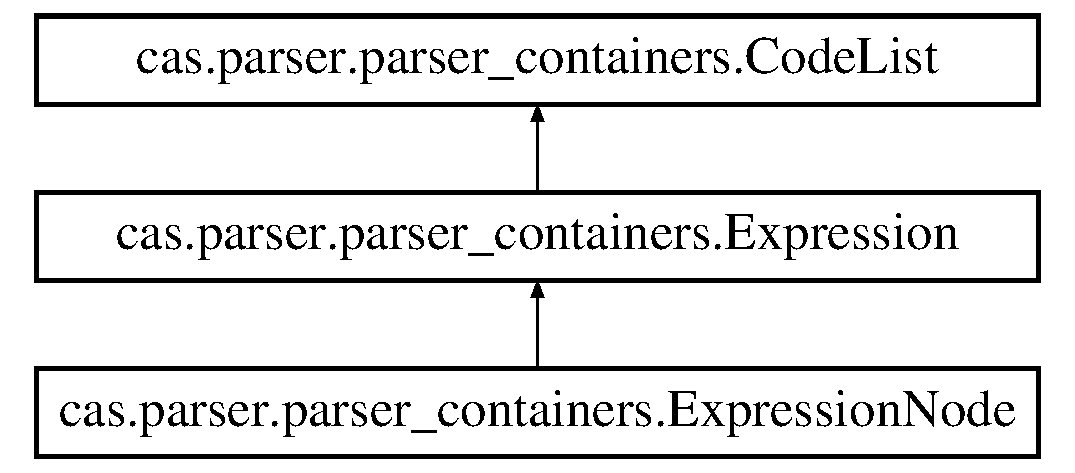
\includegraphics[height=3.000000cm]{classcas_1_1parser_1_1parser__containers_1_1_expression}
\end{center}
\end{figure}
\subsection*{Public Member Functions}
\begin{DoxyCompactItemize}
\item 
\hyperlink{classcas_1_1parser_1_1parser__containers_1_1_expression_a3000b1d4192eca32d9a6e846f4d80724}{Expression} ()
\item 
\hyperlink{classcas_1_1parser_1_1parser__containers_1_1_expression_a1942fa3e6c146e3469a8ecb00bf59f07}{Expression} (\hyperlink{classcas_1_1parser_1_1parser__containers_1_1_expression}{Expression} other\-Expression)
\item 
\hyperlink{classcas_1_1parser_1_1parser__containers_1_1_expression_af0da682360425f92a9a5c2590c26c665}{Expression} (Array\-List$<$ \hyperlink{classcas_1_1instruction_1_1_instruction}{Instruction} $>$ instructions, \hyperlink{enumcas_1_1machine_1_1_virtual_machine_1_1_var_type}{Var\-Type} \hyperlink{classcas_1_1parser_1_1parser__containers_1_1_expression_aa6d0024a94d5ac5dce65134687996048}{eval\-Type}, int \hyperlink{classcas_1_1parser_1_1parser__containers_1_1_expression_a5ca245757ba655aa1cf856670b039913}{result})
\item 
int \hyperlink{classcas_1_1parser_1_1parser__containers_1_1_expression_ad32e3e85adbd31c0a7bf4c8cc54fd807}{get\-Result\-Location} ()
\item 
boolean \hyperlink{classcas_1_1parser_1_1parser__containers_1_1_expression_a37b6a69fc045236645b29a6ea97eaa29}{has\-Result} ()
\item 
\hyperlink{enumcas_1_1machine_1_1_virtual_machine_1_1_var_type}{Var\-Type} \hyperlink{classcas_1_1parser_1_1parser__containers_1_1_expression_aa82d0811166799fe20226aa21b08d381}{eval\-Type} ()
\item 
void \hyperlink{classcas_1_1parser_1_1parser__containers_1_1_expression_a6affc96eeef61b44ab6ef45792dd8fc9}{set\-Result\-Location} (int \hyperlink{classcas_1_1parser_1_1parser__containers_1_1_expression_a5ca245757ba655aa1cf856670b039913}{result})
\item 
void \hyperlink{classcas_1_1parser_1_1parser__containers_1_1_expression_a30c794fe9ffb590f5454450abbd2940c}{null\-Result\-Location} ()
\item 
void \hyperlink{classcas_1_1parser_1_1parser__containers_1_1_expression_a967117019abe13cf427292bbd9966415}{set\-Eval\-Type} (\hyperlink{enumcas_1_1machine_1_1_virtual_machine_1_1_var_type}{Var\-Type} type)
\item 
String \hyperlink{classcas_1_1parser_1_1parser__containers_1_1_expression_aecd789d5647e365b7b24f2ca5cb53d6a}{to\-String} ()
\end{DoxyCompactItemize}
\subsection*{Protected Attributes}
\begin{DoxyCompactItemize}
\item 
\hyperlink{enumcas_1_1machine_1_1_virtual_machine_1_1_var_type}{Var\-Type} \hyperlink{classcas_1_1parser_1_1parser__containers_1_1_expression_aa6d0024a94d5ac5dce65134687996048}{eval\-Type}
\item 
int \hyperlink{classcas_1_1parser_1_1parser__containers_1_1_expression_a5ca245757ba655aa1cf856670b039913}{result}
\end{DoxyCompactItemize}


\subsection{Constructor \& Destructor Documentation}
\hypertarget{classcas_1_1parser_1_1parser__containers_1_1_expression_a3000b1d4192eca32d9a6e846f4d80724}{\index{cas\-::parser\-::parser\-\_\-containers\-::\-Expression@{cas\-::parser\-::parser\-\_\-containers\-::\-Expression}!Expression@{Expression}}
\index{Expression@{Expression}!cas::parser::parser_containers::Expression@{cas\-::parser\-::parser\-\_\-containers\-::\-Expression}}
\subsubsection[{Expression}]{\setlength{\rightskip}{0pt plus 5cm}cas.\-parser.\-parser\-\_\-containers.\-Expression.\-Expression (
\begin{DoxyParamCaption}
{}
\end{DoxyParamCaption}
)}}\label{classcas_1_1parser_1_1parser__containers_1_1_expression_a3000b1d4192eca32d9a6e846f4d80724}
\hypertarget{classcas_1_1parser_1_1parser__containers_1_1_expression_a1942fa3e6c146e3469a8ecb00bf59f07}{\index{cas\-::parser\-::parser\-\_\-containers\-::\-Expression@{cas\-::parser\-::parser\-\_\-containers\-::\-Expression}!Expression@{Expression}}
\index{Expression@{Expression}!cas::parser::parser_containers::Expression@{cas\-::parser\-::parser\-\_\-containers\-::\-Expression}}
\subsubsection[{Expression}]{\setlength{\rightskip}{0pt plus 5cm}cas.\-parser.\-parser\-\_\-containers.\-Expression.\-Expression (
\begin{DoxyParamCaption}
\item[{{\bf Expression}}]{other\-Expression}
\end{DoxyParamCaption}
)}}\label{classcas_1_1parser_1_1parser__containers_1_1_expression_a1942fa3e6c146e3469a8ecb00bf59f07}
\hypertarget{classcas_1_1parser_1_1parser__containers_1_1_expression_af0da682360425f92a9a5c2590c26c665}{\index{cas\-::parser\-::parser\-\_\-containers\-::\-Expression@{cas\-::parser\-::parser\-\_\-containers\-::\-Expression}!Expression@{Expression}}
\index{Expression@{Expression}!cas::parser::parser_containers::Expression@{cas\-::parser\-::parser\-\_\-containers\-::\-Expression}}
\subsubsection[{Expression}]{\setlength{\rightskip}{0pt plus 5cm}cas.\-parser.\-parser\-\_\-containers.\-Expression.\-Expression (
\begin{DoxyParamCaption}
\item[{Array\-List$<$ {\bf Instruction} $>$}]{instructions, }
\item[{{\bf Var\-Type}}]{eval\-Type, }
\item[{int}]{result}
\end{DoxyParamCaption}
)}}\label{classcas_1_1parser_1_1parser__containers_1_1_expression_af0da682360425f92a9a5c2590c26c665}


\subsection{Member Function Documentation}
\hypertarget{classcas_1_1parser_1_1parser__containers_1_1_expression_aa82d0811166799fe20226aa21b08d381}{\index{cas\-::parser\-::parser\-\_\-containers\-::\-Expression@{cas\-::parser\-::parser\-\_\-containers\-::\-Expression}!eval\-Type@{eval\-Type}}
\index{eval\-Type@{eval\-Type}!cas::parser::parser_containers::Expression@{cas\-::parser\-::parser\-\_\-containers\-::\-Expression}}
\subsubsection[{eval\-Type}]{\setlength{\rightskip}{0pt plus 5cm}{\bf Var\-Type} cas.\-parser.\-parser\-\_\-containers.\-Expression.\-eval\-Type (
\begin{DoxyParamCaption}
{}
\end{DoxyParamCaption}
)}}\label{classcas_1_1parser_1_1parser__containers_1_1_expression_aa82d0811166799fe20226aa21b08d381}
\hypertarget{classcas_1_1parser_1_1parser__containers_1_1_expression_ad32e3e85adbd31c0a7bf4c8cc54fd807}{\index{cas\-::parser\-::parser\-\_\-containers\-::\-Expression@{cas\-::parser\-::parser\-\_\-containers\-::\-Expression}!get\-Result\-Location@{get\-Result\-Location}}
\index{get\-Result\-Location@{get\-Result\-Location}!cas::parser::parser_containers::Expression@{cas\-::parser\-::parser\-\_\-containers\-::\-Expression}}
\subsubsection[{get\-Result\-Location}]{\setlength{\rightskip}{0pt plus 5cm}int cas.\-parser.\-parser\-\_\-containers.\-Expression.\-get\-Result\-Location (
\begin{DoxyParamCaption}
{}
\end{DoxyParamCaption}
)}}\label{classcas_1_1parser_1_1parser__containers_1_1_expression_ad32e3e85adbd31c0a7bf4c8cc54fd807}
\hypertarget{classcas_1_1parser_1_1parser__containers_1_1_expression_a37b6a69fc045236645b29a6ea97eaa29}{\index{cas\-::parser\-::parser\-\_\-containers\-::\-Expression@{cas\-::parser\-::parser\-\_\-containers\-::\-Expression}!has\-Result@{has\-Result}}
\index{has\-Result@{has\-Result}!cas::parser::parser_containers::Expression@{cas\-::parser\-::parser\-\_\-containers\-::\-Expression}}
\subsubsection[{has\-Result}]{\setlength{\rightskip}{0pt plus 5cm}boolean cas.\-parser.\-parser\-\_\-containers.\-Expression.\-has\-Result (
\begin{DoxyParamCaption}
{}
\end{DoxyParamCaption}
)}}\label{classcas_1_1parser_1_1parser__containers_1_1_expression_a37b6a69fc045236645b29a6ea97eaa29}
\hypertarget{classcas_1_1parser_1_1parser__containers_1_1_expression_a30c794fe9ffb590f5454450abbd2940c}{\index{cas\-::parser\-::parser\-\_\-containers\-::\-Expression@{cas\-::parser\-::parser\-\_\-containers\-::\-Expression}!null\-Result\-Location@{null\-Result\-Location}}
\index{null\-Result\-Location@{null\-Result\-Location}!cas::parser::parser_containers::Expression@{cas\-::parser\-::parser\-\_\-containers\-::\-Expression}}
\subsubsection[{null\-Result\-Location}]{\setlength{\rightskip}{0pt plus 5cm}void cas.\-parser.\-parser\-\_\-containers.\-Expression.\-null\-Result\-Location (
\begin{DoxyParamCaption}
{}
\end{DoxyParamCaption}
)}}\label{classcas_1_1parser_1_1parser__containers_1_1_expression_a30c794fe9ffb590f5454450abbd2940c}
\hypertarget{classcas_1_1parser_1_1parser__containers_1_1_expression_a967117019abe13cf427292bbd9966415}{\index{cas\-::parser\-::parser\-\_\-containers\-::\-Expression@{cas\-::parser\-::parser\-\_\-containers\-::\-Expression}!set\-Eval\-Type@{set\-Eval\-Type}}
\index{set\-Eval\-Type@{set\-Eval\-Type}!cas::parser::parser_containers::Expression@{cas\-::parser\-::parser\-\_\-containers\-::\-Expression}}
\subsubsection[{set\-Eval\-Type}]{\setlength{\rightskip}{0pt plus 5cm}void cas.\-parser.\-parser\-\_\-containers.\-Expression.\-set\-Eval\-Type (
\begin{DoxyParamCaption}
\item[{{\bf Var\-Type}}]{type}
\end{DoxyParamCaption}
)}}\label{classcas_1_1parser_1_1parser__containers_1_1_expression_a967117019abe13cf427292bbd9966415}
\hypertarget{classcas_1_1parser_1_1parser__containers_1_1_expression_a6affc96eeef61b44ab6ef45792dd8fc9}{\index{cas\-::parser\-::parser\-\_\-containers\-::\-Expression@{cas\-::parser\-::parser\-\_\-containers\-::\-Expression}!set\-Result\-Location@{set\-Result\-Location}}
\index{set\-Result\-Location@{set\-Result\-Location}!cas::parser::parser_containers::Expression@{cas\-::parser\-::parser\-\_\-containers\-::\-Expression}}
\subsubsection[{set\-Result\-Location}]{\setlength{\rightskip}{0pt plus 5cm}void cas.\-parser.\-parser\-\_\-containers.\-Expression.\-set\-Result\-Location (
\begin{DoxyParamCaption}
\item[{int}]{result}
\end{DoxyParamCaption}
)}}\label{classcas_1_1parser_1_1parser__containers_1_1_expression_a6affc96eeef61b44ab6ef45792dd8fc9}
\hypertarget{classcas_1_1parser_1_1parser__containers_1_1_expression_aecd789d5647e365b7b24f2ca5cb53d6a}{\index{cas\-::parser\-::parser\-\_\-containers\-::\-Expression@{cas\-::parser\-::parser\-\_\-containers\-::\-Expression}!to\-String@{to\-String}}
\index{to\-String@{to\-String}!cas::parser::parser_containers::Expression@{cas\-::parser\-::parser\-\_\-containers\-::\-Expression}}
\subsubsection[{to\-String}]{\setlength{\rightskip}{0pt plus 5cm}String cas.\-parser.\-parser\-\_\-containers.\-Expression.\-to\-String (
\begin{DoxyParamCaption}
{}
\end{DoxyParamCaption}
)}}\label{classcas_1_1parser_1_1parser__containers_1_1_expression_aecd789d5647e365b7b24f2ca5cb53d6a}


\subsection{Member Data Documentation}
\hypertarget{classcas_1_1parser_1_1parser__containers_1_1_expression_aa6d0024a94d5ac5dce65134687996048}{\index{cas\-::parser\-::parser\-\_\-containers\-::\-Expression@{cas\-::parser\-::parser\-\_\-containers\-::\-Expression}!eval\-Type@{eval\-Type}}
\index{eval\-Type@{eval\-Type}!cas::parser::parser_containers::Expression@{cas\-::parser\-::parser\-\_\-containers\-::\-Expression}}
\subsubsection[{eval\-Type}]{\setlength{\rightskip}{0pt plus 5cm}{\bf Var\-Type} cas.\-parser.\-parser\-\_\-containers.\-Expression.\-eval\-Type\hspace{0.3cm}{\ttfamily [protected]}}}\label{classcas_1_1parser_1_1parser__containers_1_1_expression_aa6d0024a94d5ac5dce65134687996048}
\hypertarget{classcas_1_1parser_1_1parser__containers_1_1_expression_a5ca245757ba655aa1cf856670b039913}{\index{cas\-::parser\-::parser\-\_\-containers\-::\-Expression@{cas\-::parser\-::parser\-\_\-containers\-::\-Expression}!result@{result}}
\index{result@{result}!cas::parser::parser_containers::Expression@{cas\-::parser\-::parser\-\_\-containers\-::\-Expression}}
\subsubsection[{result}]{\setlength{\rightskip}{0pt plus 5cm}int cas.\-parser.\-parser\-\_\-containers.\-Expression.\-result\hspace{0.3cm}{\ttfamily [protected]}}}\label{classcas_1_1parser_1_1parser__containers_1_1_expression_a5ca245757ba655aa1cf856670b039913}


The documentation for this class was generated from the following file\-:\begin{DoxyCompactItemize}
\item 
cas/parser/parser\-\_\-containers/\hyperlink{_expression_8java}{Expression.\-java}\end{DoxyCompactItemize}

\hypertarget{classcas_1_1parser_1_1parser__containers_1_1_expression_node}{\section{cas.\-parser.\-parser\-\_\-containers.\-Expression\-Node Class Reference}
\label{classcas_1_1parser_1_1parser__containers_1_1_expression_node}\index{cas.\-parser.\-parser\-\_\-containers.\-Expression\-Node@{cas.\-parser.\-parser\-\_\-containers.\-Expression\-Node}}
}
Inheritance diagram for cas.\-parser.\-parser\-\_\-containers.\-Expression\-Node\-:\begin{figure}[H]
\begin{center}
\leavevmode
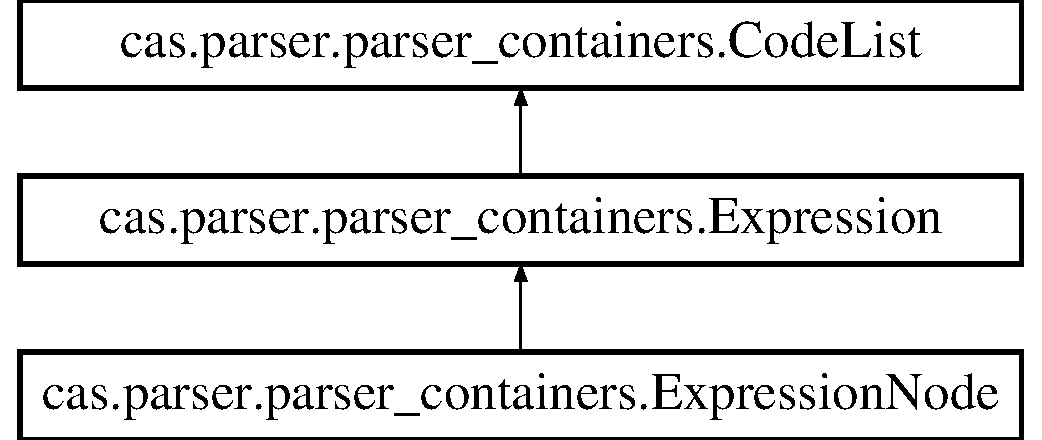
\includegraphics[height=3.000000cm]{classcas_1_1parser_1_1parser__containers_1_1_expression_node}
\end{center}
\end{figure}
\subsection*{Public Member Functions}
\begin{DoxyCompactItemize}
\item 
\hyperlink{classcas_1_1parser_1_1parser__containers_1_1_expression_node_a6aaea753a98084e9b22255ce53c31771}{Expression\-Node} ()
\item 
void \hyperlink{classcas_1_1parser_1_1parser__containers_1_1_expression_node_af37f6d1bdba8fe13b2dc9fd66d0b7414}{set\-Left\-Node} (\hyperlink{classcas_1_1parser_1_1parser__containers_1_1_expression_node}{Expression\-Node} left\-Node)
\item 
void \hyperlink{classcas_1_1parser_1_1parser__containers_1_1_expression_node_a4ccd425a9a5143f4724628185ef6070a}{set\-Right\-Node} (\hyperlink{classcas_1_1parser_1_1parser__containers_1_1_expression_node}{Expression\-Node} right\-Node)
\item 
void \hyperlink{classcas_1_1parser_1_1parser__containers_1_1_expression_node_ae873ca67bc4f88fe7f4113271bd18fee}{set\-Partial\-Instruction} (\hyperlink{classcas_1_1instruction_1_1_instruction}{Instruction} instruction)
\item 
void \hyperlink{classcas_1_1parser_1_1parser__containers_1_1_expression_node_aad8d8730a9e7c4184cc9ba4750e14ed9}{set\-Label} (int \hyperlink{classcas_1_1parser_1_1parser__containers_1_1_expression_node_ab6d6903b314dfd5b4b79ccbce24f0631}{label})
\item 
void \hyperlink{classcas_1_1parser_1_1parser__containers_1_1_expression_node_af7249a7d98cf1836aa91de98050c2854}{make\-Label} ()  throws Runtime\-Exception 
\item 
boolean \hyperlink{classcas_1_1parser_1_1parser__containers_1_1_expression_node_a0fbc1d0a05bbe68a8827be9bf35ee617}{has\-Children} ()
\item 
\hyperlink{classcas_1_1parser_1_1parser__containers_1_1_expression_node}{Expression\-Node} \hyperlink{classcas_1_1parser_1_1parser__containers_1_1_expression_node_a78b33b4902212c64b11f1efb1f9f39b8}{get\-Left\-Node} ()
\item 
\hyperlink{classcas_1_1parser_1_1parser__containers_1_1_expression_node}{Expression\-Node} \hyperlink{classcas_1_1parser_1_1parser__containers_1_1_expression_node_a04ed4ef18d9bcaedf8512577657fc856}{get\-Right\-Node} ()
\item 
int \hyperlink{classcas_1_1parser_1_1parser__containers_1_1_expression_node_adf3d73f73c910850ec7c2a0696d78503}{label} ()
\item 
\hyperlink{classcas_1_1instruction_1_1_instruction}{Instruction} \hyperlink{classcas_1_1parser_1_1parser__containers_1_1_expression_node_abe26368226d31ccbc5efdd17f3ae14d4}{partial\-Instruction} ()
\item 
\hyperlink{classcas_1_1parser_1_1parser__containers_1_1_expression}{Expression} \hyperlink{classcas_1_1parser_1_1parser__containers_1_1_expression_node_a76aa3de99fba3760b753a903b639ace1}{get\-Expression} ()
\end{DoxyCompactItemize}
\subsection*{Protected Attributes}
\begin{DoxyCompactItemize}
\item 
\hyperlink{classcas_1_1parser_1_1parser__containers_1_1_expression_node}{Expression\-Node} \hyperlink{classcas_1_1parser_1_1parser__containers_1_1_expression_node_a9ea3bb472e0892da90c7fba6d884d448}{left}
\item 
int \hyperlink{classcas_1_1parser_1_1parser__containers_1_1_expression_node_ab6d6903b314dfd5b4b79ccbce24f0631}{label}
\item 
\hyperlink{classcas_1_1instruction_1_1_instruction}{Instruction} \hyperlink{classcas_1_1parser_1_1parser__containers_1_1_expression_node_a6cbe923e93f3ddb3b0484b1625d4f003}{partial\-Instruction}
\end{DoxyCompactItemize}


\subsection{Constructor \& Destructor Documentation}
\hypertarget{classcas_1_1parser_1_1parser__containers_1_1_expression_node_a6aaea753a98084e9b22255ce53c31771}{\index{cas\-::parser\-::parser\-\_\-containers\-::\-Expression\-Node@{cas\-::parser\-::parser\-\_\-containers\-::\-Expression\-Node}!Expression\-Node@{Expression\-Node}}
\index{Expression\-Node@{Expression\-Node}!cas::parser::parser_containers::ExpressionNode@{cas\-::parser\-::parser\-\_\-containers\-::\-Expression\-Node}}
\subsubsection[{Expression\-Node}]{\setlength{\rightskip}{0pt plus 5cm}cas.\-parser.\-parser\-\_\-containers.\-Expression\-Node.\-Expression\-Node (
\begin{DoxyParamCaption}
{}
\end{DoxyParamCaption}
)}}\label{classcas_1_1parser_1_1parser__containers_1_1_expression_node_a6aaea753a98084e9b22255ce53c31771}


\subsection{Member Function Documentation}
\hypertarget{classcas_1_1parser_1_1parser__containers_1_1_expression_node_a76aa3de99fba3760b753a903b639ace1}{\index{cas\-::parser\-::parser\-\_\-containers\-::\-Expression\-Node@{cas\-::parser\-::parser\-\_\-containers\-::\-Expression\-Node}!get\-Expression@{get\-Expression}}
\index{get\-Expression@{get\-Expression}!cas::parser::parser_containers::ExpressionNode@{cas\-::parser\-::parser\-\_\-containers\-::\-Expression\-Node}}
\subsubsection[{get\-Expression}]{\setlength{\rightskip}{0pt plus 5cm}{\bf Expression} cas.\-parser.\-parser\-\_\-containers.\-Expression\-Node.\-get\-Expression (
\begin{DoxyParamCaption}
{}
\end{DoxyParamCaption}
)}}\label{classcas_1_1parser_1_1parser__containers_1_1_expression_node_a76aa3de99fba3760b753a903b639ace1}
\hypertarget{classcas_1_1parser_1_1parser__containers_1_1_expression_node_a78b33b4902212c64b11f1efb1f9f39b8}{\index{cas\-::parser\-::parser\-\_\-containers\-::\-Expression\-Node@{cas\-::parser\-::parser\-\_\-containers\-::\-Expression\-Node}!get\-Left\-Node@{get\-Left\-Node}}
\index{get\-Left\-Node@{get\-Left\-Node}!cas::parser::parser_containers::ExpressionNode@{cas\-::parser\-::parser\-\_\-containers\-::\-Expression\-Node}}
\subsubsection[{get\-Left\-Node}]{\setlength{\rightskip}{0pt plus 5cm}{\bf Expression\-Node} cas.\-parser.\-parser\-\_\-containers.\-Expression\-Node.\-get\-Left\-Node (
\begin{DoxyParamCaption}
{}
\end{DoxyParamCaption}
)}}\label{classcas_1_1parser_1_1parser__containers_1_1_expression_node_a78b33b4902212c64b11f1efb1f9f39b8}
\hypertarget{classcas_1_1parser_1_1parser__containers_1_1_expression_node_a04ed4ef18d9bcaedf8512577657fc856}{\index{cas\-::parser\-::parser\-\_\-containers\-::\-Expression\-Node@{cas\-::parser\-::parser\-\_\-containers\-::\-Expression\-Node}!get\-Right\-Node@{get\-Right\-Node}}
\index{get\-Right\-Node@{get\-Right\-Node}!cas::parser::parser_containers::ExpressionNode@{cas\-::parser\-::parser\-\_\-containers\-::\-Expression\-Node}}
\subsubsection[{get\-Right\-Node}]{\setlength{\rightskip}{0pt plus 5cm}{\bf Expression\-Node} cas.\-parser.\-parser\-\_\-containers.\-Expression\-Node.\-get\-Right\-Node (
\begin{DoxyParamCaption}
{}
\end{DoxyParamCaption}
)}}\label{classcas_1_1parser_1_1parser__containers_1_1_expression_node_a04ed4ef18d9bcaedf8512577657fc856}
\hypertarget{classcas_1_1parser_1_1parser__containers_1_1_expression_node_a0fbc1d0a05bbe68a8827be9bf35ee617}{\index{cas\-::parser\-::parser\-\_\-containers\-::\-Expression\-Node@{cas\-::parser\-::parser\-\_\-containers\-::\-Expression\-Node}!has\-Children@{has\-Children}}
\index{has\-Children@{has\-Children}!cas::parser::parser_containers::ExpressionNode@{cas\-::parser\-::parser\-\_\-containers\-::\-Expression\-Node}}
\subsubsection[{has\-Children}]{\setlength{\rightskip}{0pt plus 5cm}boolean cas.\-parser.\-parser\-\_\-containers.\-Expression\-Node.\-has\-Children (
\begin{DoxyParamCaption}
{}
\end{DoxyParamCaption}
)}}\label{classcas_1_1parser_1_1parser__containers_1_1_expression_node_a0fbc1d0a05bbe68a8827be9bf35ee617}
\hypertarget{classcas_1_1parser_1_1parser__containers_1_1_expression_node_adf3d73f73c910850ec7c2a0696d78503}{\index{cas\-::parser\-::parser\-\_\-containers\-::\-Expression\-Node@{cas\-::parser\-::parser\-\_\-containers\-::\-Expression\-Node}!label@{label}}
\index{label@{label}!cas::parser::parser_containers::ExpressionNode@{cas\-::parser\-::parser\-\_\-containers\-::\-Expression\-Node}}
\subsubsection[{label}]{\setlength{\rightskip}{0pt plus 5cm}int cas.\-parser.\-parser\-\_\-containers.\-Expression\-Node.\-label (
\begin{DoxyParamCaption}
{}
\end{DoxyParamCaption}
)}}\label{classcas_1_1parser_1_1parser__containers_1_1_expression_node_adf3d73f73c910850ec7c2a0696d78503}
\hypertarget{classcas_1_1parser_1_1parser__containers_1_1_expression_node_af7249a7d98cf1836aa91de98050c2854}{\index{cas\-::parser\-::parser\-\_\-containers\-::\-Expression\-Node@{cas\-::parser\-::parser\-\_\-containers\-::\-Expression\-Node}!make\-Label@{make\-Label}}
\index{make\-Label@{make\-Label}!cas::parser::parser_containers::ExpressionNode@{cas\-::parser\-::parser\-\_\-containers\-::\-Expression\-Node}}
\subsubsection[{make\-Label}]{\setlength{\rightskip}{0pt plus 5cm}void cas.\-parser.\-parser\-\_\-containers.\-Expression\-Node.\-make\-Label (
\begin{DoxyParamCaption}
{}
\end{DoxyParamCaption}
)  throws Runtime\-Exception }}\label{classcas_1_1parser_1_1parser__containers_1_1_expression_node_af7249a7d98cf1836aa91de98050c2854}
\hypertarget{classcas_1_1parser_1_1parser__containers_1_1_expression_node_abe26368226d31ccbc5efdd17f3ae14d4}{\index{cas\-::parser\-::parser\-\_\-containers\-::\-Expression\-Node@{cas\-::parser\-::parser\-\_\-containers\-::\-Expression\-Node}!partial\-Instruction@{partial\-Instruction}}
\index{partial\-Instruction@{partial\-Instruction}!cas::parser::parser_containers::ExpressionNode@{cas\-::parser\-::parser\-\_\-containers\-::\-Expression\-Node}}
\subsubsection[{partial\-Instruction}]{\setlength{\rightskip}{0pt plus 5cm}{\bf Instruction} cas.\-parser.\-parser\-\_\-containers.\-Expression\-Node.\-partial\-Instruction (
\begin{DoxyParamCaption}
{}
\end{DoxyParamCaption}
)}}\label{classcas_1_1parser_1_1parser__containers_1_1_expression_node_abe26368226d31ccbc5efdd17f3ae14d4}
\hypertarget{classcas_1_1parser_1_1parser__containers_1_1_expression_node_aad8d8730a9e7c4184cc9ba4750e14ed9}{\index{cas\-::parser\-::parser\-\_\-containers\-::\-Expression\-Node@{cas\-::parser\-::parser\-\_\-containers\-::\-Expression\-Node}!set\-Label@{set\-Label}}
\index{set\-Label@{set\-Label}!cas::parser::parser_containers::ExpressionNode@{cas\-::parser\-::parser\-\_\-containers\-::\-Expression\-Node}}
\subsubsection[{set\-Label}]{\setlength{\rightskip}{0pt plus 5cm}void cas.\-parser.\-parser\-\_\-containers.\-Expression\-Node.\-set\-Label (
\begin{DoxyParamCaption}
\item[{int}]{label}
\end{DoxyParamCaption}
)}}\label{classcas_1_1parser_1_1parser__containers_1_1_expression_node_aad8d8730a9e7c4184cc9ba4750e14ed9}
\hypertarget{classcas_1_1parser_1_1parser__containers_1_1_expression_node_af37f6d1bdba8fe13b2dc9fd66d0b7414}{\index{cas\-::parser\-::parser\-\_\-containers\-::\-Expression\-Node@{cas\-::parser\-::parser\-\_\-containers\-::\-Expression\-Node}!set\-Left\-Node@{set\-Left\-Node}}
\index{set\-Left\-Node@{set\-Left\-Node}!cas::parser::parser_containers::ExpressionNode@{cas\-::parser\-::parser\-\_\-containers\-::\-Expression\-Node}}
\subsubsection[{set\-Left\-Node}]{\setlength{\rightskip}{0pt plus 5cm}void cas.\-parser.\-parser\-\_\-containers.\-Expression\-Node.\-set\-Left\-Node (
\begin{DoxyParamCaption}
\item[{{\bf Expression\-Node}}]{left\-Node}
\end{DoxyParamCaption}
)}}\label{classcas_1_1parser_1_1parser__containers_1_1_expression_node_af37f6d1bdba8fe13b2dc9fd66d0b7414}
\hypertarget{classcas_1_1parser_1_1parser__containers_1_1_expression_node_ae873ca67bc4f88fe7f4113271bd18fee}{\index{cas\-::parser\-::parser\-\_\-containers\-::\-Expression\-Node@{cas\-::parser\-::parser\-\_\-containers\-::\-Expression\-Node}!set\-Partial\-Instruction@{set\-Partial\-Instruction}}
\index{set\-Partial\-Instruction@{set\-Partial\-Instruction}!cas::parser::parser_containers::ExpressionNode@{cas\-::parser\-::parser\-\_\-containers\-::\-Expression\-Node}}
\subsubsection[{set\-Partial\-Instruction}]{\setlength{\rightskip}{0pt plus 5cm}void cas.\-parser.\-parser\-\_\-containers.\-Expression\-Node.\-set\-Partial\-Instruction (
\begin{DoxyParamCaption}
\item[{{\bf Instruction}}]{instruction}
\end{DoxyParamCaption}
)}}\label{classcas_1_1parser_1_1parser__containers_1_1_expression_node_ae873ca67bc4f88fe7f4113271bd18fee}
\hypertarget{classcas_1_1parser_1_1parser__containers_1_1_expression_node_a4ccd425a9a5143f4724628185ef6070a}{\index{cas\-::parser\-::parser\-\_\-containers\-::\-Expression\-Node@{cas\-::parser\-::parser\-\_\-containers\-::\-Expression\-Node}!set\-Right\-Node@{set\-Right\-Node}}
\index{set\-Right\-Node@{set\-Right\-Node}!cas::parser::parser_containers::ExpressionNode@{cas\-::parser\-::parser\-\_\-containers\-::\-Expression\-Node}}
\subsubsection[{set\-Right\-Node}]{\setlength{\rightskip}{0pt plus 5cm}void cas.\-parser.\-parser\-\_\-containers.\-Expression\-Node.\-set\-Right\-Node (
\begin{DoxyParamCaption}
\item[{{\bf Expression\-Node}}]{right\-Node}
\end{DoxyParamCaption}
)}}\label{classcas_1_1parser_1_1parser__containers_1_1_expression_node_a4ccd425a9a5143f4724628185ef6070a}


\subsection{Member Data Documentation}
\hypertarget{classcas_1_1parser_1_1parser__containers_1_1_expression_node_ab6d6903b314dfd5b4b79ccbce24f0631}{\index{cas\-::parser\-::parser\-\_\-containers\-::\-Expression\-Node@{cas\-::parser\-::parser\-\_\-containers\-::\-Expression\-Node}!label@{label}}
\index{label@{label}!cas::parser::parser_containers::ExpressionNode@{cas\-::parser\-::parser\-\_\-containers\-::\-Expression\-Node}}
\subsubsection[{label}]{\setlength{\rightskip}{0pt plus 5cm}int cas.\-parser.\-parser\-\_\-containers.\-Expression\-Node.\-label\hspace{0.3cm}{\ttfamily [protected]}}}\label{classcas_1_1parser_1_1parser__containers_1_1_expression_node_ab6d6903b314dfd5b4b79ccbce24f0631}
\hypertarget{classcas_1_1parser_1_1parser__containers_1_1_expression_node_a9ea3bb472e0892da90c7fba6d884d448}{\index{cas\-::parser\-::parser\-\_\-containers\-::\-Expression\-Node@{cas\-::parser\-::parser\-\_\-containers\-::\-Expression\-Node}!left@{left}}
\index{left@{left}!cas::parser::parser_containers::ExpressionNode@{cas\-::parser\-::parser\-\_\-containers\-::\-Expression\-Node}}
\subsubsection[{left}]{\setlength{\rightskip}{0pt plus 5cm}{\bf Expression\-Node} cas.\-parser.\-parser\-\_\-containers.\-Expression\-Node.\-left\hspace{0.3cm}{\ttfamily [protected]}}}\label{classcas_1_1parser_1_1parser__containers_1_1_expression_node_a9ea3bb472e0892da90c7fba6d884d448}
\hypertarget{classcas_1_1parser_1_1parser__containers_1_1_expression_node_a6cbe923e93f3ddb3b0484b1625d4f003}{\index{cas\-::parser\-::parser\-\_\-containers\-::\-Expression\-Node@{cas\-::parser\-::parser\-\_\-containers\-::\-Expression\-Node}!partial\-Instruction@{partial\-Instruction}}
\index{partial\-Instruction@{partial\-Instruction}!cas::parser::parser_containers::ExpressionNode@{cas\-::parser\-::parser\-\_\-containers\-::\-Expression\-Node}}
\subsubsection[{partial\-Instruction}]{\setlength{\rightskip}{0pt plus 5cm}{\bf Instruction} cas.\-parser.\-parser\-\_\-containers.\-Expression\-Node.\-partial\-Instruction\hspace{0.3cm}{\ttfamily [protected]}}}\label{classcas_1_1parser_1_1parser__containers_1_1_expression_node_a6cbe923e93f3ddb3b0484b1625d4f003}


The documentation for this class was generated from the following file\-:\begin{DoxyCompactItemize}
\item 
cas/parser/parser\-\_\-containers/\hyperlink{_expression_node_8java}{Expression\-Node.\-java}\end{DoxyCompactItemize}

\hypertarget{classcas_1_1instruction_1_1_halt_return}{\section{cas.\-instruction.\-Halt\-Return Class Reference}
\label{classcas_1_1instruction_1_1_halt_return}\index{cas.\-instruction.\-Halt\-Return@{cas.\-instruction.\-Halt\-Return}}
}
Inheritance diagram for cas.\-instruction.\-Halt\-Return\-:\begin{figure}[H]
\begin{center}
\leavevmode
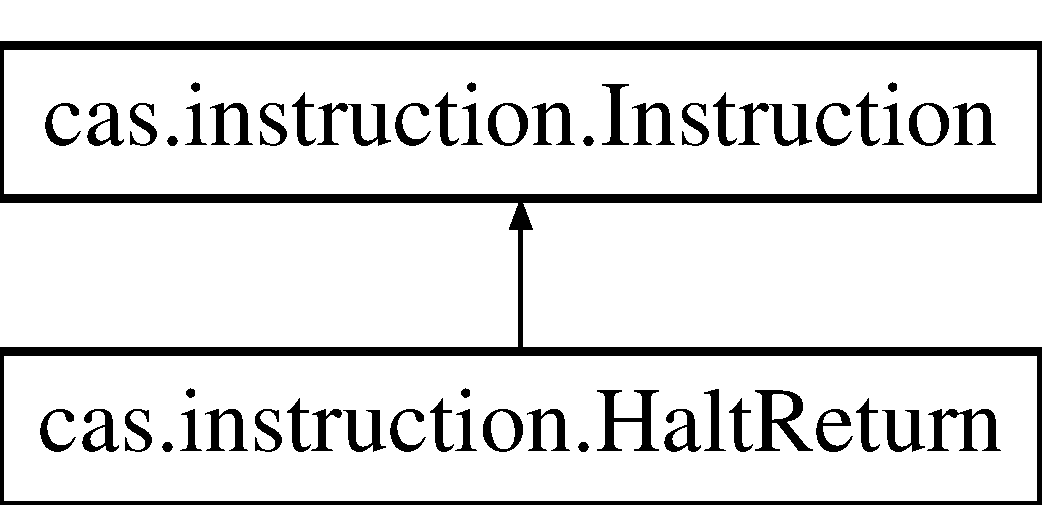
\includegraphics[height=2.000000cm]{classcas_1_1instruction_1_1_halt_return}
\end{center}
\end{figure}
\subsection*{Public Member Functions}
\begin{DoxyCompactItemize}
\item 
\hyperlink{classcas_1_1instruction_1_1_halt_return_a61338ee2f9c8b536d017a0a2460fa462}{Halt\-Return} ()
\item 
\hyperlink{classcas_1_1instruction_1_1_halt_return_a7feb7eee73e043ca07330b890261cf6f}{Halt\-Return} (int \hyperlink{classcas_1_1instruction_1_1_halt_return_a930a6b44e9c51195469ae5c0486b22c9}{return\-Register})
\item 
int \hyperlink{classcas_1_1instruction_1_1_halt_return_a930a6b44e9c51195469ae5c0486b22c9}{return\-Register} ()
\item 
void \hyperlink{classcas_1_1instruction_1_1_halt_return_ac92f107b4b3898da91bc3fa91fab5919}{set\-Return\-Register} (int register)
\item 
String \hyperlink{classcas_1_1instruction_1_1_halt_return_adceb35fd6da0f8bd54140a3c4d5019d5}{to\-String} ()
\end{DoxyCompactItemize}
\subsection*{Protected Attributes}
\begin{DoxyCompactItemize}
\item 
int \hyperlink{classcas_1_1instruction_1_1_halt_return_afd0e3bf0dd3d52b6a0982a9de9aa55d1}{return\-Reg}
\end{DoxyCompactItemize}


\subsection{Constructor \& Destructor Documentation}
\hypertarget{classcas_1_1instruction_1_1_halt_return_a61338ee2f9c8b536d017a0a2460fa462}{\index{cas\-::instruction\-::\-Halt\-Return@{cas\-::instruction\-::\-Halt\-Return}!Halt\-Return@{Halt\-Return}}
\index{Halt\-Return@{Halt\-Return}!cas::instruction::HaltReturn@{cas\-::instruction\-::\-Halt\-Return}}
\subsubsection[{Halt\-Return}]{\setlength{\rightskip}{0pt plus 5cm}cas.\-instruction.\-Halt\-Return.\-Halt\-Return (
\begin{DoxyParamCaption}
{}
\end{DoxyParamCaption}
)}}\label{classcas_1_1instruction_1_1_halt_return_a61338ee2f9c8b536d017a0a2460fa462}
\hypertarget{classcas_1_1instruction_1_1_halt_return_a7feb7eee73e043ca07330b890261cf6f}{\index{cas\-::instruction\-::\-Halt\-Return@{cas\-::instruction\-::\-Halt\-Return}!Halt\-Return@{Halt\-Return}}
\index{Halt\-Return@{Halt\-Return}!cas::instruction::HaltReturn@{cas\-::instruction\-::\-Halt\-Return}}
\subsubsection[{Halt\-Return}]{\setlength{\rightskip}{0pt plus 5cm}cas.\-instruction.\-Halt\-Return.\-Halt\-Return (
\begin{DoxyParamCaption}
\item[{int}]{return\-Register}
\end{DoxyParamCaption}
)}}\label{classcas_1_1instruction_1_1_halt_return_a7feb7eee73e043ca07330b890261cf6f}


\subsection{Member Function Documentation}
\hypertarget{classcas_1_1instruction_1_1_halt_return_a930a6b44e9c51195469ae5c0486b22c9}{\index{cas\-::instruction\-::\-Halt\-Return@{cas\-::instruction\-::\-Halt\-Return}!return\-Register@{return\-Register}}
\index{return\-Register@{return\-Register}!cas::instruction::HaltReturn@{cas\-::instruction\-::\-Halt\-Return}}
\subsubsection[{return\-Register}]{\setlength{\rightskip}{0pt plus 5cm}int cas.\-instruction.\-Halt\-Return.\-return\-Register (
\begin{DoxyParamCaption}
{}
\end{DoxyParamCaption}
)}}\label{classcas_1_1instruction_1_1_halt_return_a930a6b44e9c51195469ae5c0486b22c9}
\hypertarget{classcas_1_1instruction_1_1_halt_return_ac92f107b4b3898da91bc3fa91fab5919}{\index{cas\-::instruction\-::\-Halt\-Return@{cas\-::instruction\-::\-Halt\-Return}!set\-Return\-Register@{set\-Return\-Register}}
\index{set\-Return\-Register@{set\-Return\-Register}!cas::instruction::HaltReturn@{cas\-::instruction\-::\-Halt\-Return}}
\subsubsection[{set\-Return\-Register}]{\setlength{\rightskip}{0pt plus 5cm}void cas.\-instruction.\-Halt\-Return.\-set\-Return\-Register (
\begin{DoxyParamCaption}
\item[{int}]{register}
\end{DoxyParamCaption}
)}}\label{classcas_1_1instruction_1_1_halt_return_ac92f107b4b3898da91bc3fa91fab5919}
\hypertarget{classcas_1_1instruction_1_1_halt_return_adceb35fd6da0f8bd54140a3c4d5019d5}{\index{cas\-::instruction\-::\-Halt\-Return@{cas\-::instruction\-::\-Halt\-Return}!to\-String@{to\-String}}
\index{to\-String@{to\-String}!cas::instruction::HaltReturn@{cas\-::instruction\-::\-Halt\-Return}}
\subsubsection[{to\-String}]{\setlength{\rightskip}{0pt plus 5cm}String cas.\-instruction.\-Halt\-Return.\-to\-String (
\begin{DoxyParamCaption}
{}
\end{DoxyParamCaption}
)\hspace{0.3cm}{\ttfamily [virtual]}}}\label{classcas_1_1instruction_1_1_halt_return_adceb35fd6da0f8bd54140a3c4d5019d5}


Implements \hyperlink{classcas_1_1instruction_1_1_instruction_a7992edd8d79e1a4e82fb44f4c9abacf9}{cas.\-instruction.\-Instruction}.



\subsection{Member Data Documentation}
\hypertarget{classcas_1_1instruction_1_1_halt_return_afd0e3bf0dd3d52b6a0982a9de9aa55d1}{\index{cas\-::instruction\-::\-Halt\-Return@{cas\-::instruction\-::\-Halt\-Return}!return\-Reg@{return\-Reg}}
\index{return\-Reg@{return\-Reg}!cas::instruction::HaltReturn@{cas\-::instruction\-::\-Halt\-Return}}
\subsubsection[{return\-Reg}]{\setlength{\rightskip}{0pt plus 5cm}int cas.\-instruction.\-Halt\-Return.\-return\-Reg\hspace{0.3cm}{\ttfamily [protected]}}}\label{classcas_1_1instruction_1_1_halt_return_afd0e3bf0dd3d52b6a0982a9de9aa55d1}


The documentation for this class was generated from the following file\-:\begin{DoxyCompactItemize}
\item 
cas/instruction/\hyperlink{_halt_return_8java}{Halt\-Return.\-java}\end{DoxyCompactItemize}

\hypertarget{classcas_1_1parser_1_1parser__containers_1_1_indexable_stack_3_01_t_01_4}{\section{cas.\-parser.\-parser\-\_\-containers.\-Indexable\-Stack$<$ T $>$ Class Reference}
\label{classcas_1_1parser_1_1parser__containers_1_1_indexable_stack_3_01_t_01_4}\index{cas.\-parser.\-parser\-\_\-containers.\-Indexable\-Stack$<$ T $>$@{cas.\-parser.\-parser\-\_\-containers.\-Indexable\-Stack$<$ T $>$}}
}
\subsection*{Public Member Functions}
\begin{DoxyCompactItemize}
\item 
\hyperlink{classcas_1_1parser_1_1parser__containers_1_1_indexable_stack_3_01_t_01_4_a77cdc8a7b1328ea1a79596323748e063}{Indexable\-Stack} ()
\item 
int \hyperlink{classcas_1_1parser_1_1parser__containers_1_1_indexable_stack_3_01_t_01_4_adff8db7d2e5a71e36d3cfeaee0877e74}{push} (T object)  throws Runtime\-Exception
\item 
int \hyperlink{classcas_1_1parser_1_1parser__containers_1_1_indexable_stack_3_01_t_01_4_ae722898670ffad7e72be3156f4f1045b}{pop} ()
\item 
T \hyperlink{classcas_1_1parser_1_1parser__containers_1_1_indexable_stack_3_01_t_01_4_a73e35a0fc50450cc97490a101631c777}{get} (int i)
\item 
void \hyperlink{classcas_1_1parser_1_1parser__containers_1_1_indexable_stack_3_01_t_01_4_a42dd3c5376aab3d20ef7bae7593cc943}{set} (int i, T element)
\item 
int \hyperlink{classcas_1_1parser_1_1parser__containers_1_1_indexable_stack_3_01_t_01_4_a969637098846092ef3618a4fa21a5987}{poppable} ()
\item 
String \hyperlink{classcas_1_1parser_1_1parser__containers_1_1_indexable_stack_3_01_t_01_4_a7a3a452fbec96a81daa705e27982206d}{to\-String} ()
\end{DoxyCompactItemize}
\subsection*{Protected Attributes}
\begin{DoxyCompactItemize}
\item 
Array\-List$<$ T $>$ \hyperlink{classcas_1_1parser_1_1parser__containers_1_1_indexable_stack_3_01_t_01_4_a1c0b5f377c93609c56559585b4d8312e}{stack}
\end{DoxyCompactItemize}


\subsection{Constructor \& Destructor Documentation}
\hypertarget{classcas_1_1parser_1_1parser__containers_1_1_indexable_stack_3_01_t_01_4_a77cdc8a7b1328ea1a79596323748e063}{\index{cas\-::parser\-::parser\-\_\-containers\-::\-Indexable\-Stack$<$ T $>$@{cas\-::parser\-::parser\-\_\-containers\-::\-Indexable\-Stack$<$ T $>$}!Indexable\-Stack@{Indexable\-Stack}}
\index{Indexable\-Stack@{Indexable\-Stack}!cas::parser::parser_containers::IndexableStack< T >@{cas\-::parser\-::parser\-\_\-containers\-::\-Indexable\-Stack$<$ T $>$}}
\subsubsection[{Indexable\-Stack}]{\setlength{\rightskip}{0pt plus 5cm}cas.\-parser.\-parser\-\_\-containers.\-Indexable\-Stack$<$ T $>$.Indexable\-Stack (
\begin{DoxyParamCaption}
{}
\end{DoxyParamCaption}
)}}\label{classcas_1_1parser_1_1parser__containers_1_1_indexable_stack_3_01_t_01_4_a77cdc8a7b1328ea1a79596323748e063}


\subsection{Member Function Documentation}
\hypertarget{classcas_1_1parser_1_1parser__containers_1_1_indexable_stack_3_01_t_01_4_a73e35a0fc50450cc97490a101631c777}{\index{cas\-::parser\-::parser\-\_\-containers\-::\-Indexable\-Stack$<$ T $>$@{cas\-::parser\-::parser\-\_\-containers\-::\-Indexable\-Stack$<$ T $>$}!get@{get}}
\index{get@{get}!cas::parser::parser_containers::IndexableStack< T >@{cas\-::parser\-::parser\-\_\-containers\-::\-Indexable\-Stack$<$ T $>$}}
\subsubsection[{get}]{\setlength{\rightskip}{0pt plus 5cm}T cas.\-parser.\-parser\-\_\-containers.\-Indexable\-Stack$<$ T $>$.get (
\begin{DoxyParamCaption}
\item[{int}]{i}
\end{DoxyParamCaption}
)}}\label{classcas_1_1parser_1_1parser__containers_1_1_indexable_stack_3_01_t_01_4_a73e35a0fc50450cc97490a101631c777}
\hypertarget{classcas_1_1parser_1_1parser__containers_1_1_indexable_stack_3_01_t_01_4_ae722898670ffad7e72be3156f4f1045b}{\index{cas\-::parser\-::parser\-\_\-containers\-::\-Indexable\-Stack$<$ T $>$@{cas\-::parser\-::parser\-\_\-containers\-::\-Indexable\-Stack$<$ T $>$}!pop@{pop}}
\index{pop@{pop}!cas::parser::parser_containers::IndexableStack< T >@{cas\-::parser\-::parser\-\_\-containers\-::\-Indexable\-Stack$<$ T $>$}}
\subsubsection[{pop}]{\setlength{\rightskip}{0pt plus 5cm}int cas.\-parser.\-parser\-\_\-containers.\-Indexable\-Stack$<$ T $>$.pop (
\begin{DoxyParamCaption}
{}
\end{DoxyParamCaption}
)}}\label{classcas_1_1parser_1_1parser__containers_1_1_indexable_stack_3_01_t_01_4_ae722898670ffad7e72be3156f4f1045b}
\hypertarget{classcas_1_1parser_1_1parser__containers_1_1_indexable_stack_3_01_t_01_4_a969637098846092ef3618a4fa21a5987}{\index{cas\-::parser\-::parser\-\_\-containers\-::\-Indexable\-Stack$<$ T $>$@{cas\-::parser\-::parser\-\_\-containers\-::\-Indexable\-Stack$<$ T $>$}!poppable@{poppable}}
\index{poppable@{poppable}!cas::parser::parser_containers::IndexableStack< T >@{cas\-::parser\-::parser\-\_\-containers\-::\-Indexable\-Stack$<$ T $>$}}
\subsubsection[{poppable}]{\setlength{\rightskip}{0pt plus 5cm}int cas.\-parser.\-parser\-\_\-containers.\-Indexable\-Stack$<$ T $>$.poppable (
\begin{DoxyParamCaption}
{}
\end{DoxyParamCaption}
)}}\label{classcas_1_1parser_1_1parser__containers_1_1_indexable_stack_3_01_t_01_4_a969637098846092ef3618a4fa21a5987}
\hypertarget{classcas_1_1parser_1_1parser__containers_1_1_indexable_stack_3_01_t_01_4_adff8db7d2e5a71e36d3cfeaee0877e74}{\index{cas\-::parser\-::parser\-\_\-containers\-::\-Indexable\-Stack$<$ T $>$@{cas\-::parser\-::parser\-\_\-containers\-::\-Indexable\-Stack$<$ T $>$}!push@{push}}
\index{push@{push}!cas::parser::parser_containers::IndexableStack< T >@{cas\-::parser\-::parser\-\_\-containers\-::\-Indexable\-Stack$<$ T $>$}}
\subsubsection[{push}]{\setlength{\rightskip}{0pt plus 5cm}int cas.\-parser.\-parser\-\_\-containers.\-Indexable\-Stack$<$ T $>$.push (
\begin{DoxyParamCaption}
\item[{T}]{object}
\end{DoxyParamCaption}
)  throws Runtime\-Exception}}\label{classcas_1_1parser_1_1parser__containers_1_1_indexable_stack_3_01_t_01_4_adff8db7d2e5a71e36d3cfeaee0877e74}
\hypertarget{classcas_1_1parser_1_1parser__containers_1_1_indexable_stack_3_01_t_01_4_a42dd3c5376aab3d20ef7bae7593cc943}{\index{cas\-::parser\-::parser\-\_\-containers\-::\-Indexable\-Stack$<$ T $>$@{cas\-::parser\-::parser\-\_\-containers\-::\-Indexable\-Stack$<$ T $>$}!set@{set}}
\index{set@{set}!cas::parser::parser_containers::IndexableStack< T >@{cas\-::parser\-::parser\-\_\-containers\-::\-Indexable\-Stack$<$ T $>$}}
\subsubsection[{set}]{\setlength{\rightskip}{0pt plus 5cm}void cas.\-parser.\-parser\-\_\-containers.\-Indexable\-Stack$<$ T $>$.set (
\begin{DoxyParamCaption}
\item[{int}]{i, }
\item[{T}]{element}
\end{DoxyParamCaption}
)}}\label{classcas_1_1parser_1_1parser__containers_1_1_indexable_stack_3_01_t_01_4_a42dd3c5376aab3d20ef7bae7593cc943}
\hypertarget{classcas_1_1parser_1_1parser__containers_1_1_indexable_stack_3_01_t_01_4_a7a3a452fbec96a81daa705e27982206d}{\index{cas\-::parser\-::parser\-\_\-containers\-::\-Indexable\-Stack$<$ T $>$@{cas\-::parser\-::parser\-\_\-containers\-::\-Indexable\-Stack$<$ T $>$}!to\-String@{to\-String}}
\index{to\-String@{to\-String}!cas::parser::parser_containers::IndexableStack< T >@{cas\-::parser\-::parser\-\_\-containers\-::\-Indexable\-Stack$<$ T $>$}}
\subsubsection[{to\-String}]{\setlength{\rightskip}{0pt plus 5cm}String cas.\-parser.\-parser\-\_\-containers.\-Indexable\-Stack$<$ T $>$.to\-String (
\begin{DoxyParamCaption}
{}
\end{DoxyParamCaption}
)}}\label{classcas_1_1parser_1_1parser__containers_1_1_indexable_stack_3_01_t_01_4_a7a3a452fbec96a81daa705e27982206d}


\subsection{Member Data Documentation}
\hypertarget{classcas_1_1parser_1_1parser__containers_1_1_indexable_stack_3_01_t_01_4_a1c0b5f377c93609c56559585b4d8312e}{\index{cas\-::parser\-::parser\-\_\-containers\-::\-Indexable\-Stack$<$ T $>$@{cas\-::parser\-::parser\-\_\-containers\-::\-Indexable\-Stack$<$ T $>$}!stack@{stack}}
\index{stack@{stack}!cas::parser::parser_containers::IndexableStack< T >@{cas\-::parser\-::parser\-\_\-containers\-::\-Indexable\-Stack$<$ T $>$}}
\subsubsection[{stack}]{\setlength{\rightskip}{0pt plus 5cm}Array\-List$<$T$>$ cas.\-parser.\-parser\-\_\-containers.\-Indexable\-Stack$<$ T $>$.stack\hspace{0.3cm}{\ttfamily [protected]}}}\label{classcas_1_1parser_1_1parser__containers_1_1_indexable_stack_3_01_t_01_4_a1c0b5f377c93609c56559585b4d8312e}


The documentation for this class was generated from the following file\-:\begin{DoxyCompactItemize}
\item 
cas/parser/parser\-\_\-containers/\hyperlink{_indexable_stack_8java}{Indexable\-Stack.\-java}\end{DoxyCompactItemize}

\hypertarget{classcas_1_1instruction_1_1_instruction}{\section{cas.\-instruction.\-Instruction Class Reference}
\label{classcas_1_1instruction_1_1_instruction}\index{cas.\-instruction.\-Instruction@{cas.\-instruction.\-Instruction}}
}
Inheritance diagram for cas.\-instruction.\-Instruction\-:\begin{figure}[H]
\begin{center}
\leavevmode
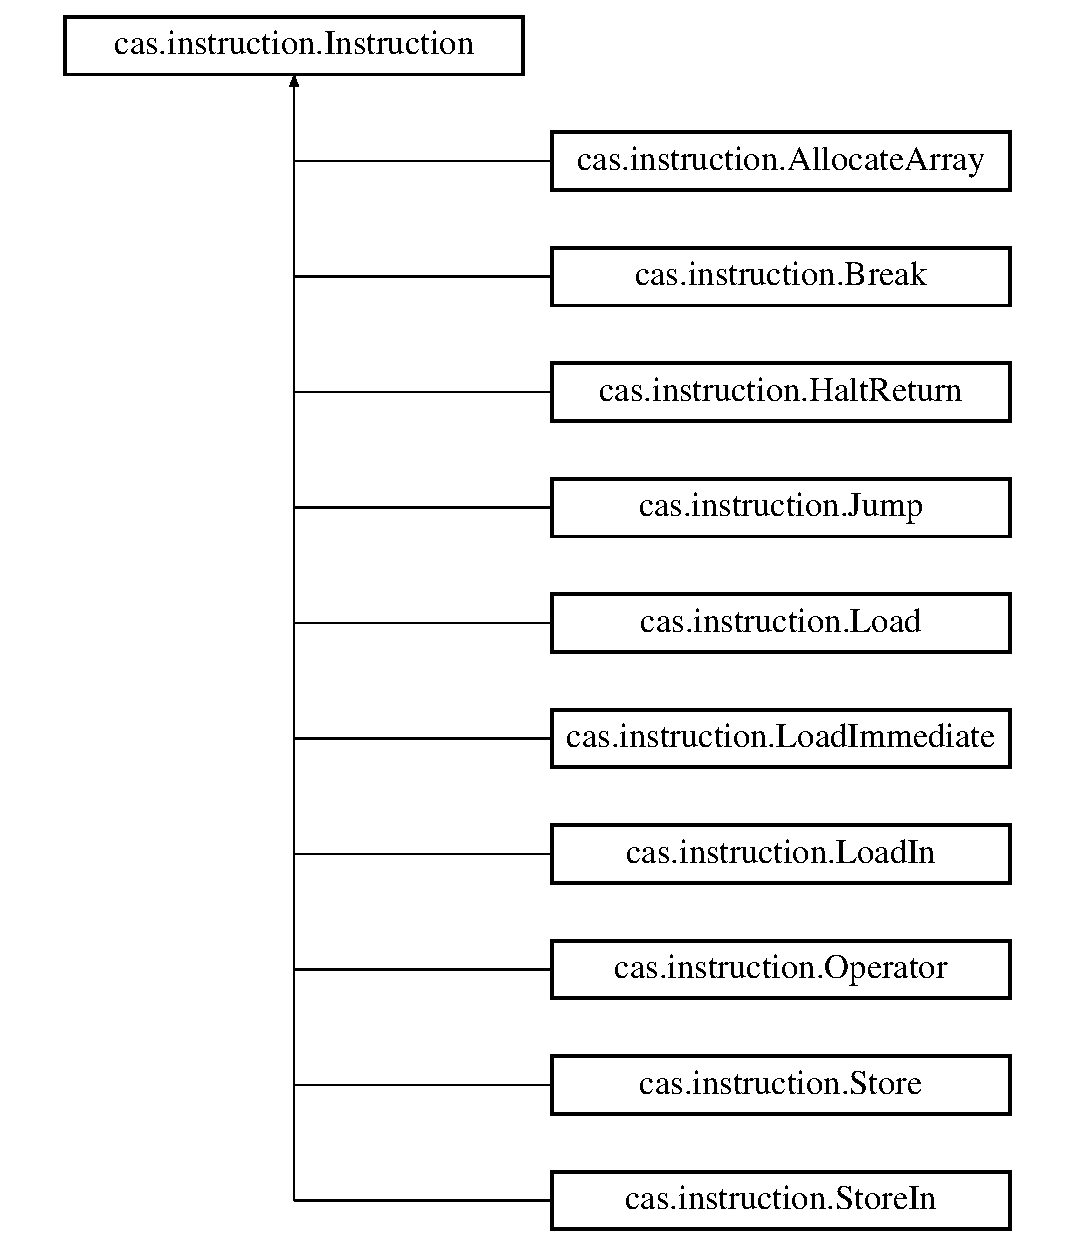
\includegraphics[height=11.000000cm]{classcas_1_1instruction_1_1_instruction}
\end{center}
\end{figure}
\subsection*{Classes}
\begin{DoxyCompactItemize}
\item 
enum \hyperlink{enumcas_1_1instruction_1_1_instruction_1_1_instruction_type}{Instruction\-Type}
\end{DoxyCompactItemize}
\subsection*{Public Member Functions}
\begin{DoxyCompactItemize}
\item 
\hyperlink{enumcas_1_1instruction_1_1_instruction_1_1_instruction_type}{Instruction\-Type} \hyperlink{classcas_1_1instruction_1_1_instruction_a3601b86fad06112c33f9e7b172e7f8f1}{get\-Type} ()
\item 
abstract String \hyperlink{classcas_1_1instruction_1_1_instruction_a7992edd8d79e1a4e82fb44f4c9abacf9}{to\-String} ()
\end{DoxyCompactItemize}


\subsection{Member Function Documentation}
\hypertarget{classcas_1_1instruction_1_1_instruction_a3601b86fad06112c33f9e7b172e7f8f1}{\index{cas\-::instruction\-::\-Instruction@{cas\-::instruction\-::\-Instruction}!get\-Type@{get\-Type}}
\index{get\-Type@{get\-Type}!cas::instruction::Instruction@{cas\-::instruction\-::\-Instruction}}
\subsubsection[{get\-Type}]{\setlength{\rightskip}{0pt plus 5cm}{\bf Instruction\-Type} cas.\-instruction.\-Instruction.\-get\-Type (
\begin{DoxyParamCaption}
{}
\end{DoxyParamCaption}
)}}\label{classcas_1_1instruction_1_1_instruction_a3601b86fad06112c33f9e7b172e7f8f1}
\hypertarget{classcas_1_1instruction_1_1_instruction_a7992edd8d79e1a4e82fb44f4c9abacf9}{\index{cas\-::instruction\-::\-Instruction@{cas\-::instruction\-::\-Instruction}!to\-String@{to\-String}}
\index{to\-String@{to\-String}!cas::instruction::Instruction@{cas\-::instruction\-::\-Instruction}}
\subsubsection[{to\-String}]{\setlength{\rightskip}{0pt plus 5cm}abstract String cas.\-instruction.\-Instruction.\-to\-String (
\begin{DoxyParamCaption}
{}
\end{DoxyParamCaption}
)\hspace{0.3cm}{\ttfamily [pure virtual]}}}\label{classcas_1_1instruction_1_1_instruction_a7992edd8d79e1a4e82fb44f4c9abacf9}


Implemented in \hyperlink{classcas_1_1instruction_1_1_operator_ab1afc1c71ba03a2530da0262f38de8b8}{cas.\-instruction.\-Operator}, \hyperlink{classcas_1_1instruction_1_1_load_in_acb274bbffd7439a3eba255ce1e793770}{cas.\-instruction.\-Load\-In}, \hyperlink{classcas_1_1instruction_1_1_store_in_aed1e070aa72b5f7ec9a11a07e4488d74}{cas.\-instruction.\-Store\-In}, \hyperlink{classcas_1_1instruction_1_1_load_a0c7010f91ddc278fe1a84522af6ffb66}{cas.\-instruction.\-Load}, \hyperlink{classcas_1_1instruction_1_1_load_immediate_a92ecadc8a40421b3fffd9ee0bb3e3cfd}{cas.\-instruction.\-Load\-Immediate}, \hyperlink{classcas_1_1instruction_1_1_store_a2b6c52613d1654df84d65e1dc1d90455}{cas.\-instruction.\-Store}, \hyperlink{classcas_1_1instruction_1_1_allocate_array_a7793a78d23230af92e5d996a6d63ee33}{cas.\-instruction.\-Allocate\-Array}, \hyperlink{classcas_1_1instruction_1_1_break_a3403130e65dafa6b1db3e7524836e6ae}{cas.\-instruction.\-Break}, \hyperlink{classcas_1_1instruction_1_1_halt_return_adceb35fd6da0f8bd54140a3c4d5019d5}{cas.\-instruction.\-Halt\-Return}, and \hyperlink{classcas_1_1instruction_1_1_jump_ab327a800e6f1817cc41e998cf555928c}{cas.\-instruction.\-Jump}.



The documentation for this class was generated from the following file\-:\begin{DoxyCompactItemize}
\item 
cas/instruction/\hyperlink{_instruction_8java}{Instruction.\-java}\end{DoxyCompactItemize}

\hypertarget{enumcas_1_1instruction_1_1_instruction_1_1_instruction_type}{\section{cas.\-instruction.\-Instruction.\-Instruction\-Type Enum Reference}
\label{enumcas_1_1instruction_1_1_instruction_1_1_instruction_type}\index{cas.\-instruction.\-Instruction.\-Instruction\-Type@{cas.\-instruction.\-Instruction.\-Instruction\-Type}}
}
\subsection*{Public Attributes}
\begin{DoxyCompactItemize}
\item 
\hyperlink{enumcas_1_1instruction_1_1_instruction_1_1_instruction_type_af90144b750051cd8d5e553f6b4a32648}{A\-L\-L\-O\-C\-A\-R\-R\-A\-Y}
\item 
\hyperlink{enumcas_1_1instruction_1_1_instruction_1_1_instruction_type_a10b70f82bf286acf173af1e1de7fc49d}{B\-R\-E\-A\-K}
\item 
\hyperlink{enumcas_1_1instruction_1_1_instruction_1_1_instruction_type_a454ae7507754cd4b6729e60caf86da76}{H\-A\-L\-T\-R\-E\-T}
\item 
\hyperlink{enumcas_1_1instruction_1_1_instruction_1_1_instruction_type_a3a302b47b2da6030ba037a906debfadb}{J\-U\-M\-P}
\item 
\hyperlink{enumcas_1_1instruction_1_1_instruction_1_1_instruction_type_aaf486500c4071599d51ce19e30fbac3a}{L\-O\-A\-D}
\item 
\hyperlink{enumcas_1_1instruction_1_1_instruction_1_1_instruction_type_aabaf7373b5f6e61e80ee49c7ee7800c7}{L\-O\-A\-D\-I\-N}
\item 
\hyperlink{enumcas_1_1instruction_1_1_instruction_1_1_instruction_type_ac58636d9948b738cb61b9a23c9701134}{L\-D\-I\-M\-M}
\item 
\hyperlink{enumcas_1_1instruction_1_1_instruction_1_1_instruction_type_a87f0dc1a1f36d5ed9372f7b9c41faf66}{S\-T\-O\-R\-E}
\item 
\hyperlink{enumcas_1_1instruction_1_1_instruction_1_1_instruction_type_a50d5585e30a38ecf7db248dea8604f44}{S\-T\-O\-R\-E\-I\-N}
\item 
\hyperlink{enumcas_1_1instruction_1_1_instruction_1_1_instruction_type_ad568056ea907e293807a1a63511b2cd1}{O\-P\-E\-R\-A\-T\-O\-R}
\end{DoxyCompactItemize}


\subsection{Member Data Documentation}
\hypertarget{enumcas_1_1instruction_1_1_instruction_1_1_instruction_type_af90144b750051cd8d5e553f6b4a32648}{\index{cas\-::instruction\-::\-Instruction\-::\-Instruction\-Type@{cas\-::instruction\-::\-Instruction\-::\-Instruction\-Type}!A\-L\-L\-O\-C\-A\-R\-R\-A\-Y@{A\-L\-L\-O\-C\-A\-R\-R\-A\-Y}}
\index{A\-L\-L\-O\-C\-A\-R\-R\-A\-Y@{A\-L\-L\-O\-C\-A\-R\-R\-A\-Y}!cas::instruction::Instruction::InstructionType@{cas\-::instruction\-::\-Instruction\-::\-Instruction\-Type}}
\subsubsection[{A\-L\-L\-O\-C\-A\-R\-R\-A\-Y}]{\setlength{\rightskip}{0pt plus 5cm}cas.\-instruction.\-Instruction.\-Instruction\-Type.\-A\-L\-L\-O\-C\-A\-R\-R\-A\-Y}}\label{enumcas_1_1instruction_1_1_instruction_1_1_instruction_type_af90144b750051cd8d5e553f6b4a32648}
\hypertarget{enumcas_1_1instruction_1_1_instruction_1_1_instruction_type_a10b70f82bf286acf173af1e1de7fc49d}{\index{cas\-::instruction\-::\-Instruction\-::\-Instruction\-Type@{cas\-::instruction\-::\-Instruction\-::\-Instruction\-Type}!B\-R\-E\-A\-K@{B\-R\-E\-A\-K}}
\index{B\-R\-E\-A\-K@{B\-R\-E\-A\-K}!cas::instruction::Instruction::InstructionType@{cas\-::instruction\-::\-Instruction\-::\-Instruction\-Type}}
\subsubsection[{B\-R\-E\-A\-K}]{\setlength{\rightskip}{0pt plus 5cm}cas.\-instruction.\-Instruction.\-Instruction\-Type.\-B\-R\-E\-A\-K}}\label{enumcas_1_1instruction_1_1_instruction_1_1_instruction_type_a10b70f82bf286acf173af1e1de7fc49d}
\hypertarget{enumcas_1_1instruction_1_1_instruction_1_1_instruction_type_a454ae7507754cd4b6729e60caf86da76}{\index{cas\-::instruction\-::\-Instruction\-::\-Instruction\-Type@{cas\-::instruction\-::\-Instruction\-::\-Instruction\-Type}!H\-A\-L\-T\-R\-E\-T@{H\-A\-L\-T\-R\-E\-T}}
\index{H\-A\-L\-T\-R\-E\-T@{H\-A\-L\-T\-R\-E\-T}!cas::instruction::Instruction::InstructionType@{cas\-::instruction\-::\-Instruction\-::\-Instruction\-Type}}
\subsubsection[{H\-A\-L\-T\-R\-E\-T}]{\setlength{\rightskip}{0pt plus 5cm}cas.\-instruction.\-Instruction.\-Instruction\-Type.\-H\-A\-L\-T\-R\-E\-T}}\label{enumcas_1_1instruction_1_1_instruction_1_1_instruction_type_a454ae7507754cd4b6729e60caf86da76}
\hypertarget{enumcas_1_1instruction_1_1_instruction_1_1_instruction_type_a3a302b47b2da6030ba037a906debfadb}{\index{cas\-::instruction\-::\-Instruction\-::\-Instruction\-Type@{cas\-::instruction\-::\-Instruction\-::\-Instruction\-Type}!J\-U\-M\-P@{J\-U\-M\-P}}
\index{J\-U\-M\-P@{J\-U\-M\-P}!cas::instruction::Instruction::InstructionType@{cas\-::instruction\-::\-Instruction\-::\-Instruction\-Type}}
\subsubsection[{J\-U\-M\-P}]{\setlength{\rightskip}{0pt plus 5cm}cas.\-instruction.\-Instruction.\-Instruction\-Type.\-J\-U\-M\-P}}\label{enumcas_1_1instruction_1_1_instruction_1_1_instruction_type_a3a302b47b2da6030ba037a906debfadb}
\hypertarget{enumcas_1_1instruction_1_1_instruction_1_1_instruction_type_ac58636d9948b738cb61b9a23c9701134}{\index{cas\-::instruction\-::\-Instruction\-::\-Instruction\-Type@{cas\-::instruction\-::\-Instruction\-::\-Instruction\-Type}!L\-D\-I\-M\-M@{L\-D\-I\-M\-M}}
\index{L\-D\-I\-M\-M@{L\-D\-I\-M\-M}!cas::instruction::Instruction::InstructionType@{cas\-::instruction\-::\-Instruction\-::\-Instruction\-Type}}
\subsubsection[{L\-D\-I\-M\-M}]{\setlength{\rightskip}{0pt plus 5cm}cas.\-instruction.\-Instruction.\-Instruction\-Type.\-L\-D\-I\-M\-M}}\label{enumcas_1_1instruction_1_1_instruction_1_1_instruction_type_ac58636d9948b738cb61b9a23c9701134}
\hypertarget{enumcas_1_1instruction_1_1_instruction_1_1_instruction_type_aaf486500c4071599d51ce19e30fbac3a}{\index{cas\-::instruction\-::\-Instruction\-::\-Instruction\-Type@{cas\-::instruction\-::\-Instruction\-::\-Instruction\-Type}!L\-O\-A\-D@{L\-O\-A\-D}}
\index{L\-O\-A\-D@{L\-O\-A\-D}!cas::instruction::Instruction::InstructionType@{cas\-::instruction\-::\-Instruction\-::\-Instruction\-Type}}
\subsubsection[{L\-O\-A\-D}]{\setlength{\rightskip}{0pt plus 5cm}cas.\-instruction.\-Instruction.\-Instruction\-Type.\-L\-O\-A\-D}}\label{enumcas_1_1instruction_1_1_instruction_1_1_instruction_type_aaf486500c4071599d51ce19e30fbac3a}
\hypertarget{enumcas_1_1instruction_1_1_instruction_1_1_instruction_type_aabaf7373b5f6e61e80ee49c7ee7800c7}{\index{cas\-::instruction\-::\-Instruction\-::\-Instruction\-Type@{cas\-::instruction\-::\-Instruction\-::\-Instruction\-Type}!L\-O\-A\-D\-I\-N@{L\-O\-A\-D\-I\-N}}
\index{L\-O\-A\-D\-I\-N@{L\-O\-A\-D\-I\-N}!cas::instruction::Instruction::InstructionType@{cas\-::instruction\-::\-Instruction\-::\-Instruction\-Type}}
\subsubsection[{L\-O\-A\-D\-I\-N}]{\setlength{\rightskip}{0pt plus 5cm}cas.\-instruction.\-Instruction.\-Instruction\-Type.\-L\-O\-A\-D\-I\-N}}\label{enumcas_1_1instruction_1_1_instruction_1_1_instruction_type_aabaf7373b5f6e61e80ee49c7ee7800c7}
\hypertarget{enumcas_1_1instruction_1_1_instruction_1_1_instruction_type_ad568056ea907e293807a1a63511b2cd1}{\index{cas\-::instruction\-::\-Instruction\-::\-Instruction\-Type@{cas\-::instruction\-::\-Instruction\-::\-Instruction\-Type}!O\-P\-E\-R\-A\-T\-O\-R@{O\-P\-E\-R\-A\-T\-O\-R}}
\index{O\-P\-E\-R\-A\-T\-O\-R@{O\-P\-E\-R\-A\-T\-O\-R}!cas::instruction::Instruction::InstructionType@{cas\-::instruction\-::\-Instruction\-::\-Instruction\-Type}}
\subsubsection[{O\-P\-E\-R\-A\-T\-O\-R}]{\setlength{\rightskip}{0pt plus 5cm}cas.\-instruction.\-Instruction.\-Instruction\-Type.\-O\-P\-E\-R\-A\-T\-O\-R}}\label{enumcas_1_1instruction_1_1_instruction_1_1_instruction_type_ad568056ea907e293807a1a63511b2cd1}
\hypertarget{enumcas_1_1instruction_1_1_instruction_1_1_instruction_type_a87f0dc1a1f36d5ed9372f7b9c41faf66}{\index{cas\-::instruction\-::\-Instruction\-::\-Instruction\-Type@{cas\-::instruction\-::\-Instruction\-::\-Instruction\-Type}!S\-T\-O\-R\-E@{S\-T\-O\-R\-E}}
\index{S\-T\-O\-R\-E@{S\-T\-O\-R\-E}!cas::instruction::Instruction::InstructionType@{cas\-::instruction\-::\-Instruction\-::\-Instruction\-Type}}
\subsubsection[{S\-T\-O\-R\-E}]{\setlength{\rightskip}{0pt plus 5cm}cas.\-instruction.\-Instruction.\-Instruction\-Type.\-S\-T\-O\-R\-E}}\label{enumcas_1_1instruction_1_1_instruction_1_1_instruction_type_a87f0dc1a1f36d5ed9372f7b9c41faf66}
\hypertarget{enumcas_1_1instruction_1_1_instruction_1_1_instruction_type_a50d5585e30a38ecf7db248dea8604f44}{\index{cas\-::instruction\-::\-Instruction\-::\-Instruction\-Type@{cas\-::instruction\-::\-Instruction\-::\-Instruction\-Type}!S\-T\-O\-R\-E\-I\-N@{S\-T\-O\-R\-E\-I\-N}}
\index{S\-T\-O\-R\-E\-I\-N@{S\-T\-O\-R\-E\-I\-N}!cas::instruction::Instruction::InstructionType@{cas\-::instruction\-::\-Instruction\-::\-Instruction\-Type}}
\subsubsection[{S\-T\-O\-R\-E\-I\-N}]{\setlength{\rightskip}{0pt plus 5cm}cas.\-instruction.\-Instruction.\-Instruction\-Type.\-S\-T\-O\-R\-E\-I\-N}}\label{enumcas_1_1instruction_1_1_instruction_1_1_instruction_type_a50d5585e30a38ecf7db248dea8604f44}


The documentation for this enum was generated from the following file\-:\begin{DoxyCompactItemize}
\item 
cas/instruction/\hyperlink{_instruction_8java}{Instruction.\-java}\end{DoxyCompactItemize}

\hypertarget{classcas_1_1instruction_1_1_jump}{\section{cas.\-instruction.\-Jump Class Reference}
\label{classcas_1_1instruction_1_1_jump}\index{cas.\-instruction.\-Jump@{cas.\-instruction.\-Jump}}
}
Inheritance diagram for cas.\-instruction.\-Jump\-:\begin{figure}[H]
\begin{center}
\leavevmode
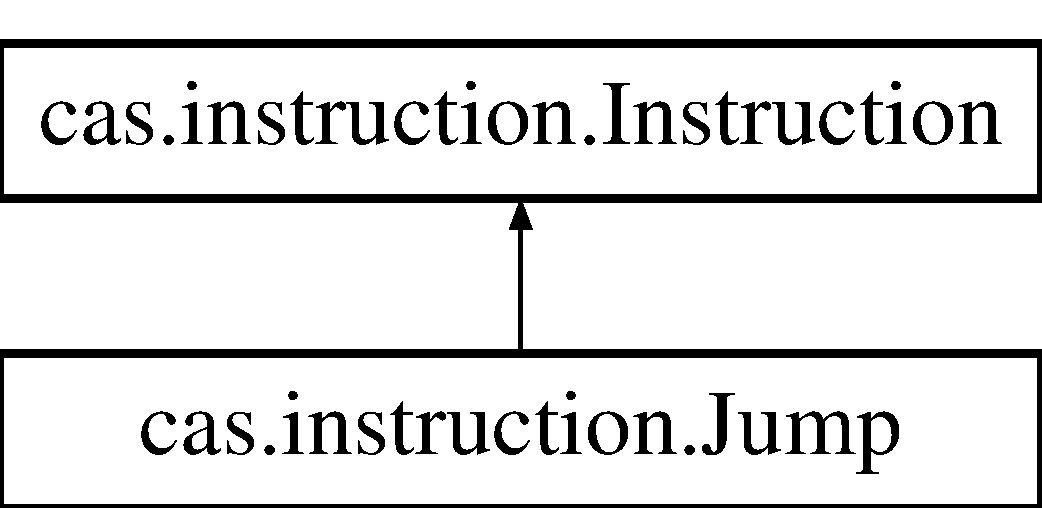
\includegraphics[height=2.000000cm]{classcas_1_1instruction_1_1_jump}
\end{center}
\end{figure}
\subsection*{Public Member Functions}
\begin{DoxyCompactItemize}
\item 
\hyperlink{classcas_1_1instruction_1_1_jump_a398865de5af8cfbd5b953c1910dacfda}{Jump} ()
\item 
\hyperlink{classcas_1_1instruction_1_1_jump_abe5311da2d382988f81d65933ff9cf44}{Jump} (int base\-Reg)
\item 
int \hyperlink{classcas_1_1instruction_1_1_jump_a8f2e48d91fb9f9cc82fdc9ac21e861dd}{get\-Base\-Register} ()
\item 
String \hyperlink{classcas_1_1instruction_1_1_jump_ab327a800e6f1817cc41e998cf555928c}{to\-String} ()
\item 
void \hyperlink{classcas_1_1instruction_1_1_jump_a699c7405303430d884232332c43b32d2}{set\-Base\-Register} (int register)
\end{DoxyCompactItemize}


\subsection{Constructor \& Destructor Documentation}
\hypertarget{classcas_1_1instruction_1_1_jump_a398865de5af8cfbd5b953c1910dacfda}{\index{cas\-::instruction\-::\-Jump@{cas\-::instruction\-::\-Jump}!Jump@{Jump}}
\index{Jump@{Jump}!cas::instruction::Jump@{cas\-::instruction\-::\-Jump}}
\subsubsection[{Jump}]{\setlength{\rightskip}{0pt plus 5cm}cas.\-instruction.\-Jump.\-Jump (
\begin{DoxyParamCaption}
{}
\end{DoxyParamCaption}
)}}\label{classcas_1_1instruction_1_1_jump_a398865de5af8cfbd5b953c1910dacfda}
\hypertarget{classcas_1_1instruction_1_1_jump_abe5311da2d382988f81d65933ff9cf44}{\index{cas\-::instruction\-::\-Jump@{cas\-::instruction\-::\-Jump}!Jump@{Jump}}
\index{Jump@{Jump}!cas::instruction::Jump@{cas\-::instruction\-::\-Jump}}
\subsubsection[{Jump}]{\setlength{\rightskip}{0pt plus 5cm}cas.\-instruction.\-Jump.\-Jump (
\begin{DoxyParamCaption}
\item[{int}]{base\-Reg}
\end{DoxyParamCaption}
)}}\label{classcas_1_1instruction_1_1_jump_abe5311da2d382988f81d65933ff9cf44}


\subsection{Member Function Documentation}
\hypertarget{classcas_1_1instruction_1_1_jump_a8f2e48d91fb9f9cc82fdc9ac21e861dd}{\index{cas\-::instruction\-::\-Jump@{cas\-::instruction\-::\-Jump}!get\-Base\-Register@{get\-Base\-Register}}
\index{get\-Base\-Register@{get\-Base\-Register}!cas::instruction::Jump@{cas\-::instruction\-::\-Jump}}
\subsubsection[{get\-Base\-Register}]{\setlength{\rightskip}{0pt plus 5cm}int cas.\-instruction.\-Jump.\-get\-Base\-Register (
\begin{DoxyParamCaption}
{}
\end{DoxyParamCaption}
)}}\label{classcas_1_1instruction_1_1_jump_a8f2e48d91fb9f9cc82fdc9ac21e861dd}
\hypertarget{classcas_1_1instruction_1_1_jump_a699c7405303430d884232332c43b32d2}{\index{cas\-::instruction\-::\-Jump@{cas\-::instruction\-::\-Jump}!set\-Base\-Register@{set\-Base\-Register}}
\index{set\-Base\-Register@{set\-Base\-Register}!cas::instruction::Jump@{cas\-::instruction\-::\-Jump}}
\subsubsection[{set\-Base\-Register}]{\setlength{\rightskip}{0pt plus 5cm}void cas.\-instruction.\-Jump.\-set\-Base\-Register (
\begin{DoxyParamCaption}
\item[{int}]{register}
\end{DoxyParamCaption}
)}}\label{classcas_1_1instruction_1_1_jump_a699c7405303430d884232332c43b32d2}
\hypertarget{classcas_1_1instruction_1_1_jump_ab327a800e6f1817cc41e998cf555928c}{\index{cas\-::instruction\-::\-Jump@{cas\-::instruction\-::\-Jump}!to\-String@{to\-String}}
\index{to\-String@{to\-String}!cas::instruction::Jump@{cas\-::instruction\-::\-Jump}}
\subsubsection[{to\-String}]{\setlength{\rightskip}{0pt plus 5cm}String cas.\-instruction.\-Jump.\-to\-String (
\begin{DoxyParamCaption}
{}
\end{DoxyParamCaption}
)\hspace{0.3cm}{\ttfamily [virtual]}}}\label{classcas_1_1instruction_1_1_jump_ab327a800e6f1817cc41e998cf555928c}


Implements \hyperlink{classcas_1_1instruction_1_1_instruction_a7992edd8d79e1a4e82fb44f4c9abacf9}{cas.\-instruction.\-Instruction}.



The documentation for this class was generated from the following file\-:\begin{DoxyCompactItemize}
\item 
cas/instruction/\hyperlink{_jump_8java}{Jump.\-java}\end{DoxyCompactItemize}

\hypertarget{classcas_1_1parser_1_1parser__containers_1_1_label}{\section{cas.\-parser.\-parser\-\_\-containers.\-Label Class Reference}
\label{classcas_1_1parser_1_1parser__containers_1_1_label}\index{cas.\-parser.\-parser\-\_\-containers.\-Label@{cas.\-parser.\-parser\-\_\-containers.\-Label}}
}
\subsection*{Public Member Functions}
\begin{DoxyCompactItemize}
\item 
String \hyperlink{classcas_1_1parser_1_1parser__containers_1_1_label_a54539628605d1c00bc33b8fc5ffe3337}{to\-String} ()
\item 
boolean \hyperlink{classcas_1_1parser_1_1parser__containers_1_1_label_a7e3f3cf6e92750bd0f9214565eba586e}{equals} (Object obj)
\item 
boolean \hyperlink{classcas_1_1parser_1_1parser__containers_1_1_label_a979e2bc705e9dc50f16a2cef6b7bc1fb}{equals} (String name)
\item 
int \hyperlink{classcas_1_1parser_1_1parser__containers_1_1_label_a231bfb254204c67918b806ba94134ead}{get\-Position} ()
\item 
String \hyperlink{classcas_1_1parser_1_1parser__containers_1_1_label_ab408647a20b45e5f4d4c9a4fb7a7e578}{get\-Name} ()
\item 
\hyperlink{enumcas_1_1machine_1_1_virtual_machine_1_1_var_type}{Var\-Type} \hyperlink{classcas_1_1parser_1_1parser__containers_1_1_label_a7b6cee4e9aacd024a93844e58ee18f22}{get\-Type} ()
\end{DoxyCompactItemize}
\subsection*{Static Public Member Functions}
\begin{DoxyCompactItemize}
\item 
static void \hyperlink{classcas_1_1parser_1_1parser__containers_1_1_label_a3a8ea18772858f0dc46dc3904ec397a4}{main} (String\mbox{[}$\,$\mbox{]} args)
\end{DoxyCompactItemize}


\subsection{Member Function Documentation}
\hypertarget{classcas_1_1parser_1_1parser__containers_1_1_label_a7e3f3cf6e92750bd0f9214565eba586e}{\index{cas\-::parser\-::parser\-\_\-containers\-::\-Label@{cas\-::parser\-::parser\-\_\-containers\-::\-Label}!equals@{equals}}
\index{equals@{equals}!cas::parser::parser_containers::Label@{cas\-::parser\-::parser\-\_\-containers\-::\-Label}}
\subsubsection[{equals}]{\setlength{\rightskip}{0pt plus 5cm}boolean cas.\-parser.\-parser\-\_\-containers.\-Label.\-equals (
\begin{DoxyParamCaption}
\item[{Object}]{obj}
\end{DoxyParamCaption}
)}}\label{classcas_1_1parser_1_1parser__containers_1_1_label_a7e3f3cf6e92750bd0f9214565eba586e}
\hypertarget{classcas_1_1parser_1_1parser__containers_1_1_label_a979e2bc705e9dc50f16a2cef6b7bc1fb}{\index{cas\-::parser\-::parser\-\_\-containers\-::\-Label@{cas\-::parser\-::parser\-\_\-containers\-::\-Label}!equals@{equals}}
\index{equals@{equals}!cas::parser::parser_containers::Label@{cas\-::parser\-::parser\-\_\-containers\-::\-Label}}
\subsubsection[{equals}]{\setlength{\rightskip}{0pt plus 5cm}boolean cas.\-parser.\-parser\-\_\-containers.\-Label.\-equals (
\begin{DoxyParamCaption}
\item[{String}]{name}
\end{DoxyParamCaption}
)}}\label{classcas_1_1parser_1_1parser__containers_1_1_label_a979e2bc705e9dc50f16a2cef6b7bc1fb}
\hypertarget{classcas_1_1parser_1_1parser__containers_1_1_label_ab408647a20b45e5f4d4c9a4fb7a7e578}{\index{cas\-::parser\-::parser\-\_\-containers\-::\-Label@{cas\-::parser\-::parser\-\_\-containers\-::\-Label}!get\-Name@{get\-Name}}
\index{get\-Name@{get\-Name}!cas::parser::parser_containers::Label@{cas\-::parser\-::parser\-\_\-containers\-::\-Label}}
\subsubsection[{get\-Name}]{\setlength{\rightskip}{0pt plus 5cm}String cas.\-parser.\-parser\-\_\-containers.\-Label.\-get\-Name (
\begin{DoxyParamCaption}
{}
\end{DoxyParamCaption}
)}}\label{classcas_1_1parser_1_1parser__containers_1_1_label_ab408647a20b45e5f4d4c9a4fb7a7e578}
\hypertarget{classcas_1_1parser_1_1parser__containers_1_1_label_a231bfb254204c67918b806ba94134ead}{\index{cas\-::parser\-::parser\-\_\-containers\-::\-Label@{cas\-::parser\-::parser\-\_\-containers\-::\-Label}!get\-Position@{get\-Position}}
\index{get\-Position@{get\-Position}!cas::parser::parser_containers::Label@{cas\-::parser\-::parser\-\_\-containers\-::\-Label}}
\subsubsection[{get\-Position}]{\setlength{\rightskip}{0pt plus 5cm}int cas.\-parser.\-parser\-\_\-containers.\-Label.\-get\-Position (
\begin{DoxyParamCaption}
{}
\end{DoxyParamCaption}
)}}\label{classcas_1_1parser_1_1parser__containers_1_1_label_a231bfb254204c67918b806ba94134ead}
\hypertarget{classcas_1_1parser_1_1parser__containers_1_1_label_a7b6cee4e9aacd024a93844e58ee18f22}{\index{cas\-::parser\-::parser\-\_\-containers\-::\-Label@{cas\-::parser\-::parser\-\_\-containers\-::\-Label}!get\-Type@{get\-Type}}
\index{get\-Type@{get\-Type}!cas::parser::parser_containers::Label@{cas\-::parser\-::parser\-\_\-containers\-::\-Label}}
\subsubsection[{get\-Type}]{\setlength{\rightskip}{0pt plus 5cm}{\bf Var\-Type} cas.\-parser.\-parser\-\_\-containers.\-Label.\-get\-Type (
\begin{DoxyParamCaption}
{}
\end{DoxyParamCaption}
)}}\label{classcas_1_1parser_1_1parser__containers_1_1_label_a7b6cee4e9aacd024a93844e58ee18f22}
\hypertarget{classcas_1_1parser_1_1parser__containers_1_1_label_a3a8ea18772858f0dc46dc3904ec397a4}{\index{cas\-::parser\-::parser\-\_\-containers\-::\-Label@{cas\-::parser\-::parser\-\_\-containers\-::\-Label}!main@{main}}
\index{main@{main}!cas::parser::parser_containers::Label@{cas\-::parser\-::parser\-\_\-containers\-::\-Label}}
\subsubsection[{main}]{\setlength{\rightskip}{0pt plus 5cm}static void cas.\-parser.\-parser\-\_\-containers.\-Label.\-main (
\begin{DoxyParamCaption}
\item[{String\mbox{[}$\,$\mbox{]}}]{args}
\end{DoxyParamCaption}
)\hspace{0.3cm}{\ttfamily [static]}}}\label{classcas_1_1parser_1_1parser__containers_1_1_label_a3a8ea18772858f0dc46dc3904ec397a4}
\hypertarget{classcas_1_1parser_1_1parser__containers_1_1_label_a54539628605d1c00bc33b8fc5ffe3337}{\index{cas\-::parser\-::parser\-\_\-containers\-::\-Label@{cas\-::parser\-::parser\-\_\-containers\-::\-Label}!to\-String@{to\-String}}
\index{to\-String@{to\-String}!cas::parser::parser_containers::Label@{cas\-::parser\-::parser\-\_\-containers\-::\-Label}}
\subsubsection[{to\-String}]{\setlength{\rightskip}{0pt plus 5cm}String cas.\-parser.\-parser\-\_\-containers.\-Label.\-to\-String (
\begin{DoxyParamCaption}
{}
\end{DoxyParamCaption}
)}}\label{classcas_1_1parser_1_1parser__containers_1_1_label_a54539628605d1c00bc33b8fc5ffe3337}


The documentation for this class was generated from the following file\-:\begin{DoxyCompactItemize}
\item 
cas/parser/parser\-\_\-containers/\hyperlink{_label_8java}{Label.\-java}\end{DoxyCompactItemize}

\hypertarget{classcas_1_1instruction_1_1_load}{\section{cas.\-instruction.\-Load Class Reference}
\label{classcas_1_1instruction_1_1_load}\index{cas.\-instruction.\-Load@{cas.\-instruction.\-Load}}
}
Inheritance diagram for cas.\-instruction.\-Load\-:\begin{figure}[H]
\begin{center}
\leavevmode
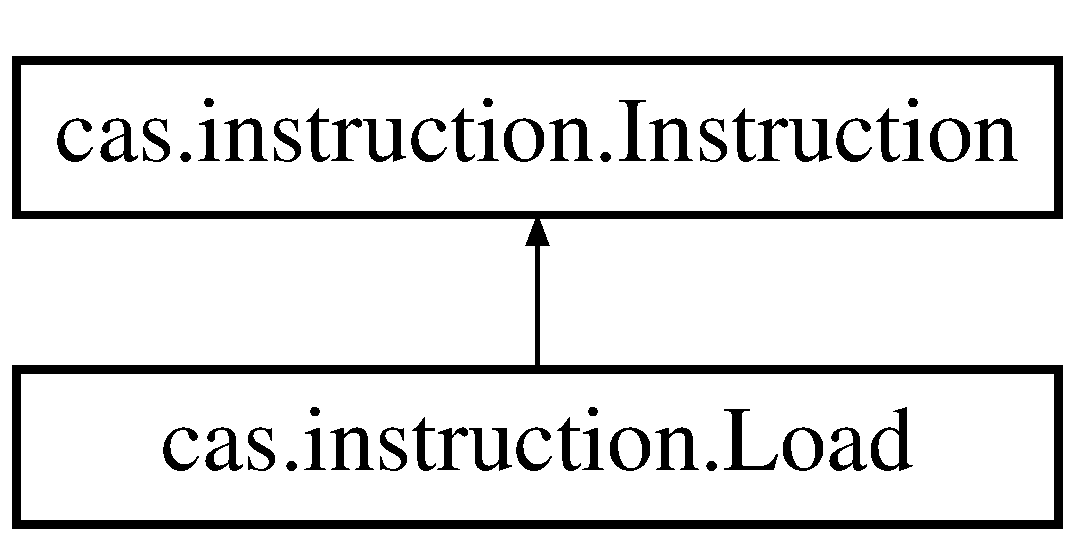
\includegraphics[height=2.000000cm]{classcas_1_1instruction_1_1_load}
\end{center}
\end{figure}
\subsection*{Public Member Functions}
\begin{DoxyCompactItemize}
\item 
\hyperlink{classcas_1_1instruction_1_1_load_afe769ce60f78ad457927170eb1202d00}{Load} ()
\item 
\hyperlink{classcas_1_1instruction_1_1_load_a545861724500b0c966383a784b11c5d9}{Load} (int source\-Index, int dest\-Reg)
\item 
int \hyperlink{classcas_1_1instruction_1_1_load_a0370a97cbe673be91a14ec3ff0f80a28}{get\-Source} ()
\item 
int \hyperlink{classcas_1_1instruction_1_1_load_a77a27b4e046a19c645769fd7aae122c2}{get\-Destination} ()
\item 
void \hyperlink{classcas_1_1instruction_1_1_load_a145a282bb473f1463d0845295d195ccc}{set\-Source} (int memory\-Location)
\item 
void \hyperlink{classcas_1_1instruction_1_1_load_abcd647e5b9c359bd13b1e057c761c95b}{set\-Destination} (int register)
\item 
String \hyperlink{classcas_1_1instruction_1_1_load_a0c7010f91ddc278fe1a84522af6ffb66}{to\-String} ()
\end{DoxyCompactItemize}


\subsection{Constructor \& Destructor Documentation}
\hypertarget{classcas_1_1instruction_1_1_load_afe769ce60f78ad457927170eb1202d00}{\index{cas\-::instruction\-::\-Load@{cas\-::instruction\-::\-Load}!Load@{Load}}
\index{Load@{Load}!cas::instruction::Load@{cas\-::instruction\-::\-Load}}
\subsubsection[{Load}]{\setlength{\rightskip}{0pt plus 5cm}cas.\-instruction.\-Load.\-Load (
\begin{DoxyParamCaption}
{}
\end{DoxyParamCaption}
)}}\label{classcas_1_1instruction_1_1_load_afe769ce60f78ad457927170eb1202d00}
\hypertarget{classcas_1_1instruction_1_1_load_a545861724500b0c966383a784b11c5d9}{\index{cas\-::instruction\-::\-Load@{cas\-::instruction\-::\-Load}!Load@{Load}}
\index{Load@{Load}!cas::instruction::Load@{cas\-::instruction\-::\-Load}}
\subsubsection[{Load}]{\setlength{\rightskip}{0pt plus 5cm}cas.\-instruction.\-Load.\-Load (
\begin{DoxyParamCaption}
\item[{int}]{source\-Index, }
\item[{int}]{dest\-Reg}
\end{DoxyParamCaption}
)}}\label{classcas_1_1instruction_1_1_load_a545861724500b0c966383a784b11c5d9}


\subsection{Member Function Documentation}
\hypertarget{classcas_1_1instruction_1_1_load_a77a27b4e046a19c645769fd7aae122c2}{\index{cas\-::instruction\-::\-Load@{cas\-::instruction\-::\-Load}!get\-Destination@{get\-Destination}}
\index{get\-Destination@{get\-Destination}!cas::instruction::Load@{cas\-::instruction\-::\-Load}}
\subsubsection[{get\-Destination}]{\setlength{\rightskip}{0pt plus 5cm}int cas.\-instruction.\-Load.\-get\-Destination (
\begin{DoxyParamCaption}
{}
\end{DoxyParamCaption}
)}}\label{classcas_1_1instruction_1_1_load_a77a27b4e046a19c645769fd7aae122c2}
\hypertarget{classcas_1_1instruction_1_1_load_a0370a97cbe673be91a14ec3ff0f80a28}{\index{cas\-::instruction\-::\-Load@{cas\-::instruction\-::\-Load}!get\-Source@{get\-Source}}
\index{get\-Source@{get\-Source}!cas::instruction::Load@{cas\-::instruction\-::\-Load}}
\subsubsection[{get\-Source}]{\setlength{\rightskip}{0pt plus 5cm}int cas.\-instruction.\-Load.\-get\-Source (
\begin{DoxyParamCaption}
{}
\end{DoxyParamCaption}
)}}\label{classcas_1_1instruction_1_1_load_a0370a97cbe673be91a14ec3ff0f80a28}
\hypertarget{classcas_1_1instruction_1_1_load_abcd647e5b9c359bd13b1e057c761c95b}{\index{cas\-::instruction\-::\-Load@{cas\-::instruction\-::\-Load}!set\-Destination@{set\-Destination}}
\index{set\-Destination@{set\-Destination}!cas::instruction::Load@{cas\-::instruction\-::\-Load}}
\subsubsection[{set\-Destination}]{\setlength{\rightskip}{0pt plus 5cm}void cas.\-instruction.\-Load.\-set\-Destination (
\begin{DoxyParamCaption}
\item[{int}]{register}
\end{DoxyParamCaption}
)}}\label{classcas_1_1instruction_1_1_load_abcd647e5b9c359bd13b1e057c761c95b}
\hypertarget{classcas_1_1instruction_1_1_load_a145a282bb473f1463d0845295d195ccc}{\index{cas\-::instruction\-::\-Load@{cas\-::instruction\-::\-Load}!set\-Source@{set\-Source}}
\index{set\-Source@{set\-Source}!cas::instruction::Load@{cas\-::instruction\-::\-Load}}
\subsubsection[{set\-Source}]{\setlength{\rightskip}{0pt plus 5cm}void cas.\-instruction.\-Load.\-set\-Source (
\begin{DoxyParamCaption}
\item[{int}]{memory\-Location}
\end{DoxyParamCaption}
)}}\label{classcas_1_1instruction_1_1_load_a145a282bb473f1463d0845295d195ccc}
\hypertarget{classcas_1_1instruction_1_1_load_a0c7010f91ddc278fe1a84522af6ffb66}{\index{cas\-::instruction\-::\-Load@{cas\-::instruction\-::\-Load}!to\-String@{to\-String}}
\index{to\-String@{to\-String}!cas::instruction::Load@{cas\-::instruction\-::\-Load}}
\subsubsection[{to\-String}]{\setlength{\rightskip}{0pt plus 5cm}String cas.\-instruction.\-Load.\-to\-String (
\begin{DoxyParamCaption}
{}
\end{DoxyParamCaption}
)\hspace{0.3cm}{\ttfamily [virtual]}}}\label{classcas_1_1instruction_1_1_load_a0c7010f91ddc278fe1a84522af6ffb66}


Implements \hyperlink{classcas_1_1instruction_1_1_instruction_a7992edd8d79e1a4e82fb44f4c9abacf9}{cas.\-instruction.\-Instruction}.



The documentation for this class was generated from the following file\-:\begin{DoxyCompactItemize}
\item 
cas/instruction/\hyperlink{_load_8java}{Load.\-java}\end{DoxyCompactItemize}

\hypertarget{classcas_1_1instruction_1_1_load_immediate}{\section{cas.\-instruction.\-Load\-Immediate Class Reference}
\label{classcas_1_1instruction_1_1_load_immediate}\index{cas.\-instruction.\-Load\-Immediate@{cas.\-instruction.\-Load\-Immediate}}
}
Inheritance diagram for cas.\-instruction.\-Load\-Immediate\-:\begin{figure}[H]
\begin{center}
\leavevmode
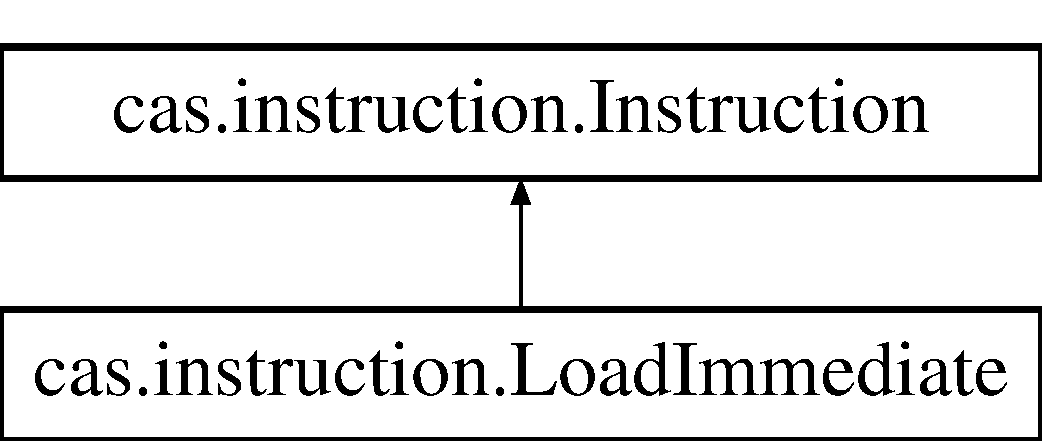
\includegraphics[height=2.000000cm]{classcas_1_1instruction_1_1_load_immediate}
\end{center}
\end{figure}
\subsection*{Public Member Functions}
\begin{DoxyCompactItemize}
\item 
\hyperlink{classcas_1_1instruction_1_1_load_immediate_ae02e96bf1e903b64f8922bbb56f662e6}{Load\-Immediate} ()
\item 
\hyperlink{classcas_1_1instruction_1_1_load_immediate_ae46e3993eba5fb51f6786a7795ec59eb}{Load\-Immediate} (int destination\-Register, Object value)
\item 
int \hyperlink{classcas_1_1instruction_1_1_load_immediate_a8668d8c66547e77dc78f78d70ef59904}{get\-Destination} ()
\item 
Object \hyperlink{classcas_1_1instruction_1_1_load_immediate_ae4ad3cb6692135efa2bcf3e53dc004c1}{get\-Value} ()
\item 
void \hyperlink{classcas_1_1instruction_1_1_load_immediate_a3049950382f8cc92298b5d0233347676}{set\-Destination} (int register)
\item 
void \hyperlink{classcas_1_1instruction_1_1_load_immediate_a42b8b2a8a2f37e715f8cadcd2c8b38b6}{set\-Value} (Object value)
\item 
String \hyperlink{classcas_1_1instruction_1_1_load_immediate_a92ecadc8a40421b3fffd9ee0bb3e3cfd}{to\-String} ()
\end{DoxyCompactItemize}


\subsection{Constructor \& Destructor Documentation}
\hypertarget{classcas_1_1instruction_1_1_load_immediate_ae02e96bf1e903b64f8922bbb56f662e6}{\index{cas\-::instruction\-::\-Load\-Immediate@{cas\-::instruction\-::\-Load\-Immediate}!Load\-Immediate@{Load\-Immediate}}
\index{Load\-Immediate@{Load\-Immediate}!cas::instruction::LoadImmediate@{cas\-::instruction\-::\-Load\-Immediate}}
\subsubsection[{Load\-Immediate}]{\setlength{\rightskip}{0pt plus 5cm}cas.\-instruction.\-Load\-Immediate.\-Load\-Immediate (
\begin{DoxyParamCaption}
{}
\end{DoxyParamCaption}
)}}\label{classcas_1_1instruction_1_1_load_immediate_ae02e96bf1e903b64f8922bbb56f662e6}
\hypertarget{classcas_1_1instruction_1_1_load_immediate_ae46e3993eba5fb51f6786a7795ec59eb}{\index{cas\-::instruction\-::\-Load\-Immediate@{cas\-::instruction\-::\-Load\-Immediate}!Load\-Immediate@{Load\-Immediate}}
\index{Load\-Immediate@{Load\-Immediate}!cas::instruction::LoadImmediate@{cas\-::instruction\-::\-Load\-Immediate}}
\subsubsection[{Load\-Immediate}]{\setlength{\rightskip}{0pt plus 5cm}cas.\-instruction.\-Load\-Immediate.\-Load\-Immediate (
\begin{DoxyParamCaption}
\item[{int}]{destination\-Register, }
\item[{Object}]{value}
\end{DoxyParamCaption}
)}}\label{classcas_1_1instruction_1_1_load_immediate_ae46e3993eba5fb51f6786a7795ec59eb}


\subsection{Member Function Documentation}
\hypertarget{classcas_1_1instruction_1_1_load_immediate_a8668d8c66547e77dc78f78d70ef59904}{\index{cas\-::instruction\-::\-Load\-Immediate@{cas\-::instruction\-::\-Load\-Immediate}!get\-Destination@{get\-Destination}}
\index{get\-Destination@{get\-Destination}!cas::instruction::LoadImmediate@{cas\-::instruction\-::\-Load\-Immediate}}
\subsubsection[{get\-Destination}]{\setlength{\rightskip}{0pt plus 5cm}int cas.\-instruction.\-Load\-Immediate.\-get\-Destination (
\begin{DoxyParamCaption}
{}
\end{DoxyParamCaption}
)}}\label{classcas_1_1instruction_1_1_load_immediate_a8668d8c66547e77dc78f78d70ef59904}
\hypertarget{classcas_1_1instruction_1_1_load_immediate_ae4ad3cb6692135efa2bcf3e53dc004c1}{\index{cas\-::instruction\-::\-Load\-Immediate@{cas\-::instruction\-::\-Load\-Immediate}!get\-Value@{get\-Value}}
\index{get\-Value@{get\-Value}!cas::instruction::LoadImmediate@{cas\-::instruction\-::\-Load\-Immediate}}
\subsubsection[{get\-Value}]{\setlength{\rightskip}{0pt plus 5cm}Object cas.\-instruction.\-Load\-Immediate.\-get\-Value (
\begin{DoxyParamCaption}
{}
\end{DoxyParamCaption}
)}}\label{classcas_1_1instruction_1_1_load_immediate_ae4ad3cb6692135efa2bcf3e53dc004c1}
\hypertarget{classcas_1_1instruction_1_1_load_immediate_a3049950382f8cc92298b5d0233347676}{\index{cas\-::instruction\-::\-Load\-Immediate@{cas\-::instruction\-::\-Load\-Immediate}!set\-Destination@{set\-Destination}}
\index{set\-Destination@{set\-Destination}!cas::instruction::LoadImmediate@{cas\-::instruction\-::\-Load\-Immediate}}
\subsubsection[{set\-Destination}]{\setlength{\rightskip}{0pt plus 5cm}void cas.\-instruction.\-Load\-Immediate.\-set\-Destination (
\begin{DoxyParamCaption}
\item[{int}]{register}
\end{DoxyParamCaption}
)}}\label{classcas_1_1instruction_1_1_load_immediate_a3049950382f8cc92298b5d0233347676}
\hypertarget{classcas_1_1instruction_1_1_load_immediate_a42b8b2a8a2f37e715f8cadcd2c8b38b6}{\index{cas\-::instruction\-::\-Load\-Immediate@{cas\-::instruction\-::\-Load\-Immediate}!set\-Value@{set\-Value}}
\index{set\-Value@{set\-Value}!cas::instruction::LoadImmediate@{cas\-::instruction\-::\-Load\-Immediate}}
\subsubsection[{set\-Value}]{\setlength{\rightskip}{0pt plus 5cm}void cas.\-instruction.\-Load\-Immediate.\-set\-Value (
\begin{DoxyParamCaption}
\item[{Object}]{value}
\end{DoxyParamCaption}
)}}\label{classcas_1_1instruction_1_1_load_immediate_a42b8b2a8a2f37e715f8cadcd2c8b38b6}
\hypertarget{classcas_1_1instruction_1_1_load_immediate_a92ecadc8a40421b3fffd9ee0bb3e3cfd}{\index{cas\-::instruction\-::\-Load\-Immediate@{cas\-::instruction\-::\-Load\-Immediate}!to\-String@{to\-String}}
\index{to\-String@{to\-String}!cas::instruction::LoadImmediate@{cas\-::instruction\-::\-Load\-Immediate}}
\subsubsection[{to\-String}]{\setlength{\rightskip}{0pt plus 5cm}String cas.\-instruction.\-Load\-Immediate.\-to\-String (
\begin{DoxyParamCaption}
{}
\end{DoxyParamCaption}
)\hspace{0.3cm}{\ttfamily [virtual]}}}\label{classcas_1_1instruction_1_1_load_immediate_a92ecadc8a40421b3fffd9ee0bb3e3cfd}


Implements \hyperlink{classcas_1_1instruction_1_1_instruction_a7992edd8d79e1a4e82fb44f4c9abacf9}{cas.\-instruction.\-Instruction}.



The documentation for this class was generated from the following file\-:\begin{DoxyCompactItemize}
\item 
cas/instruction/\hyperlink{_load_immediate_8java}{Load\-Immediate.\-java}\end{DoxyCompactItemize}

\hypertarget{classcas_1_1instruction_1_1_load_in}{\section{cas.\-instruction.\-Load\-In Class Reference}
\label{classcas_1_1instruction_1_1_load_in}\index{cas.\-instruction.\-Load\-In@{cas.\-instruction.\-Load\-In}}
}
Inheritance diagram for cas.\-instruction.\-Load\-In\-:\begin{figure}[H]
\begin{center}
\leavevmode
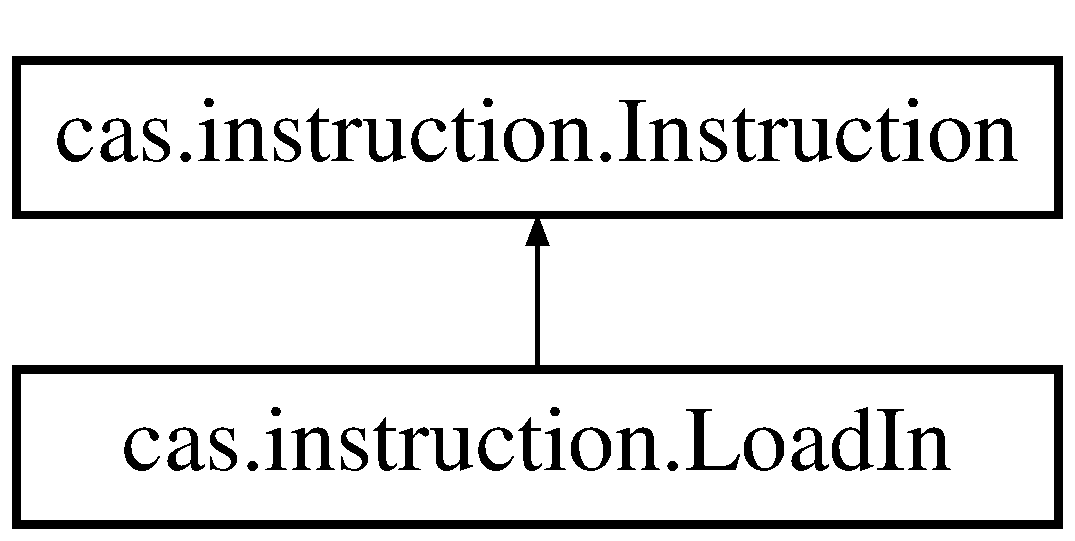
\includegraphics[height=2.000000cm]{classcas_1_1instruction_1_1_load_in}
\end{center}
\end{figure}
\subsection*{Public Member Functions}
\begin{DoxyCompactItemize}
\item 
\hyperlink{classcas_1_1instruction_1_1_load_in_a047b0ba4c79c574bd1e6752c8f4a1388}{Load\-In} ()
\item 
\hyperlink{classcas_1_1instruction_1_1_load_in_acee6f54813789963b35b995ea82a56b3}{Load\-In} (int source\-Index, int offset\-Reg, int dest\-Reg)
\item 
int \hyperlink{classcas_1_1instruction_1_1_load_in_ae9ceefd2aa26cf50289fd57f4dabe790}{get\-Source} ()
\item 
int \hyperlink{classcas_1_1instruction_1_1_load_in_a224ec4b85db568b4a2605f9533adaa51}{get\-Offset} ()
\item 
int \hyperlink{classcas_1_1instruction_1_1_load_in_a368ea01ce4dcda9bba15e501283439ca}{get\-Destination} ()
\item 
void \hyperlink{classcas_1_1instruction_1_1_load_in_a9d173070b68fcb6aea046c09a368e6b7}{set\-Source} (int memory\-Location)
\item 
void \hyperlink{classcas_1_1instruction_1_1_load_in_a8ce9a43f8e44f9e0b8edf3b1d7c654c4}{set\-Offset} (int register)
\item 
void \hyperlink{classcas_1_1instruction_1_1_load_in_a2547e43f950df15508488ce2b6013be9}{set\-Destination} (int register)
\item 
String \hyperlink{classcas_1_1instruction_1_1_load_in_acb274bbffd7439a3eba255ce1e793770}{to\-String} ()
\end{DoxyCompactItemize}


\subsection{Constructor \& Destructor Documentation}
\hypertarget{classcas_1_1instruction_1_1_load_in_a047b0ba4c79c574bd1e6752c8f4a1388}{\index{cas\-::instruction\-::\-Load\-In@{cas\-::instruction\-::\-Load\-In}!Load\-In@{Load\-In}}
\index{Load\-In@{Load\-In}!cas::instruction::LoadIn@{cas\-::instruction\-::\-Load\-In}}
\subsubsection[{Load\-In}]{\setlength{\rightskip}{0pt plus 5cm}cas.\-instruction.\-Load\-In.\-Load\-In (
\begin{DoxyParamCaption}
{}
\end{DoxyParamCaption}
)}}\label{classcas_1_1instruction_1_1_load_in_a047b0ba4c79c574bd1e6752c8f4a1388}
\hypertarget{classcas_1_1instruction_1_1_load_in_acee6f54813789963b35b995ea82a56b3}{\index{cas\-::instruction\-::\-Load\-In@{cas\-::instruction\-::\-Load\-In}!Load\-In@{Load\-In}}
\index{Load\-In@{Load\-In}!cas::instruction::LoadIn@{cas\-::instruction\-::\-Load\-In}}
\subsubsection[{Load\-In}]{\setlength{\rightskip}{0pt plus 5cm}cas.\-instruction.\-Load\-In.\-Load\-In (
\begin{DoxyParamCaption}
\item[{int}]{source\-Index, }
\item[{int}]{offset\-Reg, }
\item[{int}]{dest\-Reg}
\end{DoxyParamCaption}
)}}\label{classcas_1_1instruction_1_1_load_in_acee6f54813789963b35b995ea82a56b3}


\subsection{Member Function Documentation}
\hypertarget{classcas_1_1instruction_1_1_load_in_a368ea01ce4dcda9bba15e501283439ca}{\index{cas\-::instruction\-::\-Load\-In@{cas\-::instruction\-::\-Load\-In}!get\-Destination@{get\-Destination}}
\index{get\-Destination@{get\-Destination}!cas::instruction::LoadIn@{cas\-::instruction\-::\-Load\-In}}
\subsubsection[{get\-Destination}]{\setlength{\rightskip}{0pt plus 5cm}int cas.\-instruction.\-Load\-In.\-get\-Destination (
\begin{DoxyParamCaption}
{}
\end{DoxyParamCaption}
)}}\label{classcas_1_1instruction_1_1_load_in_a368ea01ce4dcda9bba15e501283439ca}
\hypertarget{classcas_1_1instruction_1_1_load_in_a224ec4b85db568b4a2605f9533adaa51}{\index{cas\-::instruction\-::\-Load\-In@{cas\-::instruction\-::\-Load\-In}!get\-Offset@{get\-Offset}}
\index{get\-Offset@{get\-Offset}!cas::instruction::LoadIn@{cas\-::instruction\-::\-Load\-In}}
\subsubsection[{get\-Offset}]{\setlength{\rightskip}{0pt plus 5cm}int cas.\-instruction.\-Load\-In.\-get\-Offset (
\begin{DoxyParamCaption}
{}
\end{DoxyParamCaption}
)}}\label{classcas_1_1instruction_1_1_load_in_a224ec4b85db568b4a2605f9533adaa51}
\hypertarget{classcas_1_1instruction_1_1_load_in_ae9ceefd2aa26cf50289fd57f4dabe790}{\index{cas\-::instruction\-::\-Load\-In@{cas\-::instruction\-::\-Load\-In}!get\-Source@{get\-Source}}
\index{get\-Source@{get\-Source}!cas::instruction::LoadIn@{cas\-::instruction\-::\-Load\-In}}
\subsubsection[{get\-Source}]{\setlength{\rightskip}{0pt plus 5cm}int cas.\-instruction.\-Load\-In.\-get\-Source (
\begin{DoxyParamCaption}
{}
\end{DoxyParamCaption}
)}}\label{classcas_1_1instruction_1_1_load_in_ae9ceefd2aa26cf50289fd57f4dabe790}
\hypertarget{classcas_1_1instruction_1_1_load_in_a2547e43f950df15508488ce2b6013be9}{\index{cas\-::instruction\-::\-Load\-In@{cas\-::instruction\-::\-Load\-In}!set\-Destination@{set\-Destination}}
\index{set\-Destination@{set\-Destination}!cas::instruction::LoadIn@{cas\-::instruction\-::\-Load\-In}}
\subsubsection[{set\-Destination}]{\setlength{\rightskip}{0pt plus 5cm}void cas.\-instruction.\-Load\-In.\-set\-Destination (
\begin{DoxyParamCaption}
\item[{int}]{register}
\end{DoxyParamCaption}
)}}\label{classcas_1_1instruction_1_1_load_in_a2547e43f950df15508488ce2b6013be9}
\hypertarget{classcas_1_1instruction_1_1_load_in_a8ce9a43f8e44f9e0b8edf3b1d7c654c4}{\index{cas\-::instruction\-::\-Load\-In@{cas\-::instruction\-::\-Load\-In}!set\-Offset@{set\-Offset}}
\index{set\-Offset@{set\-Offset}!cas::instruction::LoadIn@{cas\-::instruction\-::\-Load\-In}}
\subsubsection[{set\-Offset}]{\setlength{\rightskip}{0pt plus 5cm}void cas.\-instruction.\-Load\-In.\-set\-Offset (
\begin{DoxyParamCaption}
\item[{int}]{register}
\end{DoxyParamCaption}
)}}\label{classcas_1_1instruction_1_1_load_in_a8ce9a43f8e44f9e0b8edf3b1d7c654c4}
\hypertarget{classcas_1_1instruction_1_1_load_in_a9d173070b68fcb6aea046c09a368e6b7}{\index{cas\-::instruction\-::\-Load\-In@{cas\-::instruction\-::\-Load\-In}!set\-Source@{set\-Source}}
\index{set\-Source@{set\-Source}!cas::instruction::LoadIn@{cas\-::instruction\-::\-Load\-In}}
\subsubsection[{set\-Source}]{\setlength{\rightskip}{0pt plus 5cm}void cas.\-instruction.\-Load\-In.\-set\-Source (
\begin{DoxyParamCaption}
\item[{int}]{memory\-Location}
\end{DoxyParamCaption}
)}}\label{classcas_1_1instruction_1_1_load_in_a9d173070b68fcb6aea046c09a368e6b7}
\hypertarget{classcas_1_1instruction_1_1_load_in_acb274bbffd7439a3eba255ce1e793770}{\index{cas\-::instruction\-::\-Load\-In@{cas\-::instruction\-::\-Load\-In}!to\-String@{to\-String}}
\index{to\-String@{to\-String}!cas::instruction::LoadIn@{cas\-::instruction\-::\-Load\-In}}
\subsubsection[{to\-String}]{\setlength{\rightskip}{0pt plus 5cm}String cas.\-instruction.\-Load\-In.\-to\-String (
\begin{DoxyParamCaption}
{}
\end{DoxyParamCaption}
)\hspace{0.3cm}{\ttfamily [virtual]}}}\label{classcas_1_1instruction_1_1_load_in_acb274bbffd7439a3eba255ce1e793770}


Implements \hyperlink{classcas_1_1instruction_1_1_instruction_a7992edd8d79e1a4e82fb44f4c9abacf9}{cas.\-instruction.\-Instruction}.



The documentation for this class was generated from the following file\-:\begin{DoxyCompactItemize}
\item 
cas/instruction/\hyperlink{_load_in_8java}{Load\-In.\-java}\end{DoxyCompactItemize}

\hypertarget{enumcas_1_1instruction_1_1_operator_1_1_operation}{\section{cas.\-instruction.\-Operator.\-Operation Enum Reference}
\label{enumcas_1_1instruction_1_1_operator_1_1_operation}\index{cas.\-instruction.\-Operator.\-Operation@{cas.\-instruction.\-Operator.\-Operation}}
}
\subsection*{Public Attributes}
\begin{DoxyCompactItemize}
\item 
\hyperlink{enumcas_1_1instruction_1_1_operator_1_1_operation_a913f6c7e9a127ba4c988c8c66ac56bb8}{P\-L\-U\-S}
\item 
\hyperlink{enumcas_1_1instruction_1_1_operator_1_1_operation_adfb410fa8cfee05f1359aa7af5898b70}{M\-I\-N\-U\-S}
\item 
\hyperlink{enumcas_1_1instruction_1_1_operator_1_1_operation_a2b08437555339e464fdeffc9dbbde68d}{T\-I\-M\-E\-S}
\item 
\hyperlink{enumcas_1_1instruction_1_1_operator_1_1_operation_ad6116eecb86a01fa99db461fec44da3e}{D\-I\-V\-I\-D\-E}
\item 
\hyperlink{enumcas_1_1instruction_1_1_operator_1_1_operation_a20eea59278d9d18fe1b14c9e0d19aea1}{M\-O\-D}
\item 
\hyperlink{enumcas_1_1instruction_1_1_operator_1_1_operation_a2d610c17fb28c5feae027aebe25006f2}{E\-Q}
\item 
\hyperlink{enumcas_1_1instruction_1_1_operator_1_1_operation_a14636507d2e02eec58a93273a359a15a}{N\-E\-Q}
\item 
\hyperlink{enumcas_1_1instruction_1_1_operator_1_1_operation_ad938ac9e4078e59766281a3466c411a0}{L\-T}
\item 
\hyperlink{enumcas_1_1instruction_1_1_operator_1_1_operation_a6da738dd3d3efde3339d7eaa18de627f}{L\-E}
\item 
\hyperlink{enumcas_1_1instruction_1_1_operator_1_1_operation_afe4d75c3d8d4aa843f4e066011c1b0a6}{A\-N\-D}
\item 
\hyperlink{enumcas_1_1instruction_1_1_operator_1_1_operation_ad585e9c3a6e718d322803d6312a27b50}{O\-R}
\item 
\hyperlink{enumcas_1_1instruction_1_1_operator_1_1_operation_adcaa466f402ba31eb1422aedd9944403}{N\-O\-T}
\end{DoxyCompactItemize}


\subsection{Member Data Documentation}
\hypertarget{enumcas_1_1instruction_1_1_operator_1_1_operation_afe4d75c3d8d4aa843f4e066011c1b0a6}{\index{cas\-::instruction\-::\-Operator\-::\-Operation@{cas\-::instruction\-::\-Operator\-::\-Operation}!A\-N\-D@{A\-N\-D}}
\index{A\-N\-D@{A\-N\-D}!cas::instruction::Operator::Operation@{cas\-::instruction\-::\-Operator\-::\-Operation}}
\subsubsection[{A\-N\-D}]{\setlength{\rightskip}{0pt plus 5cm}cas.\-instruction.\-Operator.\-Operation.\-A\-N\-D}}\label{enumcas_1_1instruction_1_1_operator_1_1_operation_afe4d75c3d8d4aa843f4e066011c1b0a6}
\hypertarget{enumcas_1_1instruction_1_1_operator_1_1_operation_ad6116eecb86a01fa99db461fec44da3e}{\index{cas\-::instruction\-::\-Operator\-::\-Operation@{cas\-::instruction\-::\-Operator\-::\-Operation}!D\-I\-V\-I\-D\-E@{D\-I\-V\-I\-D\-E}}
\index{D\-I\-V\-I\-D\-E@{D\-I\-V\-I\-D\-E}!cas::instruction::Operator::Operation@{cas\-::instruction\-::\-Operator\-::\-Operation}}
\subsubsection[{D\-I\-V\-I\-D\-E}]{\setlength{\rightskip}{0pt plus 5cm}cas.\-instruction.\-Operator.\-Operation.\-D\-I\-V\-I\-D\-E}}\label{enumcas_1_1instruction_1_1_operator_1_1_operation_ad6116eecb86a01fa99db461fec44da3e}
\hypertarget{enumcas_1_1instruction_1_1_operator_1_1_operation_a2d610c17fb28c5feae027aebe25006f2}{\index{cas\-::instruction\-::\-Operator\-::\-Operation@{cas\-::instruction\-::\-Operator\-::\-Operation}!E\-Q@{E\-Q}}
\index{E\-Q@{E\-Q}!cas::instruction::Operator::Operation@{cas\-::instruction\-::\-Operator\-::\-Operation}}
\subsubsection[{E\-Q}]{\setlength{\rightskip}{0pt plus 5cm}cas.\-instruction.\-Operator.\-Operation.\-E\-Q}}\label{enumcas_1_1instruction_1_1_operator_1_1_operation_a2d610c17fb28c5feae027aebe25006f2}
\hypertarget{enumcas_1_1instruction_1_1_operator_1_1_operation_a6da738dd3d3efde3339d7eaa18de627f}{\index{cas\-::instruction\-::\-Operator\-::\-Operation@{cas\-::instruction\-::\-Operator\-::\-Operation}!L\-E@{L\-E}}
\index{L\-E@{L\-E}!cas::instruction::Operator::Operation@{cas\-::instruction\-::\-Operator\-::\-Operation}}
\subsubsection[{L\-E}]{\setlength{\rightskip}{0pt plus 5cm}cas.\-instruction.\-Operator.\-Operation.\-L\-E}}\label{enumcas_1_1instruction_1_1_operator_1_1_operation_a6da738dd3d3efde3339d7eaa18de627f}
\hypertarget{enumcas_1_1instruction_1_1_operator_1_1_operation_ad938ac9e4078e59766281a3466c411a0}{\index{cas\-::instruction\-::\-Operator\-::\-Operation@{cas\-::instruction\-::\-Operator\-::\-Operation}!L\-T@{L\-T}}
\index{L\-T@{L\-T}!cas::instruction::Operator::Operation@{cas\-::instruction\-::\-Operator\-::\-Operation}}
\subsubsection[{L\-T}]{\setlength{\rightskip}{0pt plus 5cm}cas.\-instruction.\-Operator.\-Operation.\-L\-T}}\label{enumcas_1_1instruction_1_1_operator_1_1_operation_ad938ac9e4078e59766281a3466c411a0}
\hypertarget{enumcas_1_1instruction_1_1_operator_1_1_operation_adfb410fa8cfee05f1359aa7af5898b70}{\index{cas\-::instruction\-::\-Operator\-::\-Operation@{cas\-::instruction\-::\-Operator\-::\-Operation}!M\-I\-N\-U\-S@{M\-I\-N\-U\-S}}
\index{M\-I\-N\-U\-S@{M\-I\-N\-U\-S}!cas::instruction::Operator::Operation@{cas\-::instruction\-::\-Operator\-::\-Operation}}
\subsubsection[{M\-I\-N\-U\-S}]{\setlength{\rightskip}{0pt plus 5cm}cas.\-instruction.\-Operator.\-Operation.\-M\-I\-N\-U\-S}}\label{enumcas_1_1instruction_1_1_operator_1_1_operation_adfb410fa8cfee05f1359aa7af5898b70}
\hypertarget{enumcas_1_1instruction_1_1_operator_1_1_operation_a20eea59278d9d18fe1b14c9e0d19aea1}{\index{cas\-::instruction\-::\-Operator\-::\-Operation@{cas\-::instruction\-::\-Operator\-::\-Operation}!M\-O\-D@{M\-O\-D}}
\index{M\-O\-D@{M\-O\-D}!cas::instruction::Operator::Operation@{cas\-::instruction\-::\-Operator\-::\-Operation}}
\subsubsection[{M\-O\-D}]{\setlength{\rightskip}{0pt plus 5cm}cas.\-instruction.\-Operator.\-Operation.\-M\-O\-D}}\label{enumcas_1_1instruction_1_1_operator_1_1_operation_a20eea59278d9d18fe1b14c9e0d19aea1}
\hypertarget{enumcas_1_1instruction_1_1_operator_1_1_operation_a14636507d2e02eec58a93273a359a15a}{\index{cas\-::instruction\-::\-Operator\-::\-Operation@{cas\-::instruction\-::\-Operator\-::\-Operation}!N\-E\-Q@{N\-E\-Q}}
\index{N\-E\-Q@{N\-E\-Q}!cas::instruction::Operator::Operation@{cas\-::instruction\-::\-Operator\-::\-Operation}}
\subsubsection[{N\-E\-Q}]{\setlength{\rightskip}{0pt plus 5cm}cas.\-instruction.\-Operator.\-Operation.\-N\-E\-Q}}\label{enumcas_1_1instruction_1_1_operator_1_1_operation_a14636507d2e02eec58a93273a359a15a}
\hypertarget{enumcas_1_1instruction_1_1_operator_1_1_operation_adcaa466f402ba31eb1422aedd9944403}{\index{cas\-::instruction\-::\-Operator\-::\-Operation@{cas\-::instruction\-::\-Operator\-::\-Operation}!N\-O\-T@{N\-O\-T}}
\index{N\-O\-T@{N\-O\-T}!cas::instruction::Operator::Operation@{cas\-::instruction\-::\-Operator\-::\-Operation}}
\subsubsection[{N\-O\-T}]{\setlength{\rightskip}{0pt plus 5cm}cas.\-instruction.\-Operator.\-Operation.\-N\-O\-T}}\label{enumcas_1_1instruction_1_1_operator_1_1_operation_adcaa466f402ba31eb1422aedd9944403}
\hypertarget{enumcas_1_1instruction_1_1_operator_1_1_operation_ad585e9c3a6e718d322803d6312a27b50}{\index{cas\-::instruction\-::\-Operator\-::\-Operation@{cas\-::instruction\-::\-Operator\-::\-Operation}!O\-R@{O\-R}}
\index{O\-R@{O\-R}!cas::instruction::Operator::Operation@{cas\-::instruction\-::\-Operator\-::\-Operation}}
\subsubsection[{O\-R}]{\setlength{\rightskip}{0pt plus 5cm}cas.\-instruction.\-Operator.\-Operation.\-O\-R}}\label{enumcas_1_1instruction_1_1_operator_1_1_operation_ad585e9c3a6e718d322803d6312a27b50}
\hypertarget{enumcas_1_1instruction_1_1_operator_1_1_operation_a913f6c7e9a127ba4c988c8c66ac56bb8}{\index{cas\-::instruction\-::\-Operator\-::\-Operation@{cas\-::instruction\-::\-Operator\-::\-Operation}!P\-L\-U\-S@{P\-L\-U\-S}}
\index{P\-L\-U\-S@{P\-L\-U\-S}!cas::instruction::Operator::Operation@{cas\-::instruction\-::\-Operator\-::\-Operation}}
\subsubsection[{P\-L\-U\-S}]{\setlength{\rightskip}{0pt plus 5cm}cas.\-instruction.\-Operator.\-Operation.\-P\-L\-U\-S}}\label{enumcas_1_1instruction_1_1_operator_1_1_operation_a913f6c7e9a127ba4c988c8c66ac56bb8}
\hypertarget{enumcas_1_1instruction_1_1_operator_1_1_operation_a2b08437555339e464fdeffc9dbbde68d}{\index{cas\-::instruction\-::\-Operator\-::\-Operation@{cas\-::instruction\-::\-Operator\-::\-Operation}!T\-I\-M\-E\-S@{T\-I\-M\-E\-S}}
\index{T\-I\-M\-E\-S@{T\-I\-M\-E\-S}!cas::instruction::Operator::Operation@{cas\-::instruction\-::\-Operator\-::\-Operation}}
\subsubsection[{T\-I\-M\-E\-S}]{\setlength{\rightskip}{0pt plus 5cm}cas.\-instruction.\-Operator.\-Operation.\-T\-I\-M\-E\-S}}\label{enumcas_1_1instruction_1_1_operator_1_1_operation_a2b08437555339e464fdeffc9dbbde68d}


The documentation for this enum was generated from the following file\-:\begin{DoxyCompactItemize}
\item 
cas/instruction/\hyperlink{_operator_8java}{Operator.\-java}\end{DoxyCompactItemize}

\hypertarget{classcas_1_1instruction_1_1_operator}{\section{cas.\-instruction.\-Operator Class Reference}
\label{classcas_1_1instruction_1_1_operator}\index{cas.\-instruction.\-Operator@{cas.\-instruction.\-Operator}}
}
Inheritance diagram for cas.\-instruction.\-Operator\-:\begin{figure}[H]
\begin{center}
\leavevmode
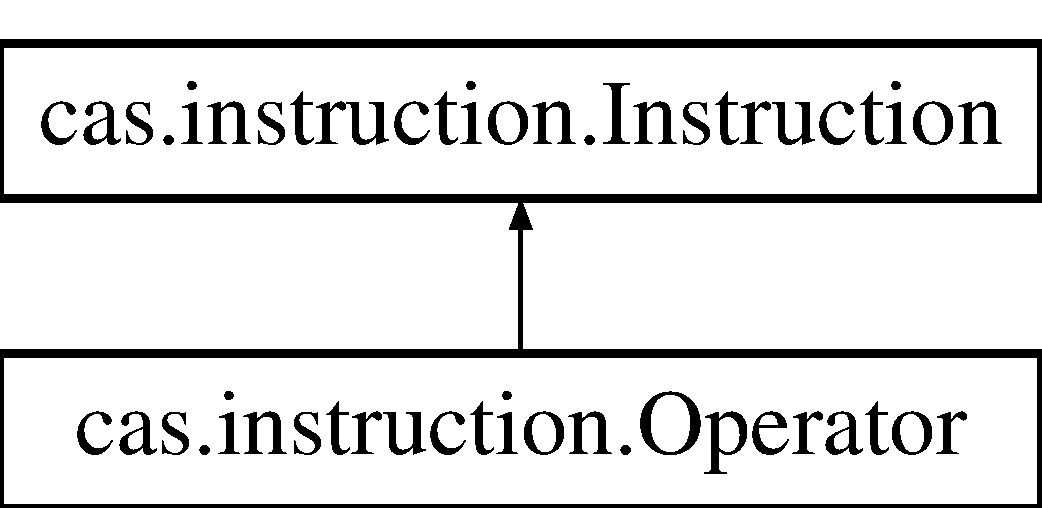
\includegraphics[height=2.000000cm]{classcas_1_1instruction_1_1_operator}
\end{center}
\end{figure}
\subsection*{Classes}
\begin{DoxyCompactItemize}
\item 
enum \hyperlink{enumcas_1_1instruction_1_1_operator_1_1_operation}{Operation}
\end{DoxyCompactItemize}
\subsection*{Public Member Functions}
\begin{DoxyCompactItemize}
\item 
\hyperlink{classcas_1_1instruction_1_1_operator_ac16250f07e727c330a3d9037ff5ac9d2}{Operator} ()
\item 
\hyperlink{classcas_1_1instruction_1_1_operator_a7f08029e4d41bfb5483622e2fdeeef9c}{Operator} (\hyperlink{enumcas_1_1instruction_1_1_operator_1_1_operation}{Operation} operator, int source\-Reg1, int source\-Reg2, int dest\-Reg)
\item 
int \hyperlink{classcas_1_1instruction_1_1_operator_a6e923a661ff6a8294041191d5a6ec09a}{get\-Source1} ()
\item 
int \hyperlink{classcas_1_1instruction_1_1_operator_a89b4ad47d31879f8fe534d8dbd85be35}{get\-Source2} ()
\item 
int \hyperlink{classcas_1_1instruction_1_1_operator_a5820e4ce3a2ee8410fb0c83a512ad75e}{get\-Destination} ()
\item 
\hyperlink{enumcas_1_1instruction_1_1_operator_1_1_operation}{Operation} \hyperlink{classcas_1_1instruction_1_1_operator_a3551a41353847f24bc0ca7c246f47c41}{get\-Operator} ()
\item 
void \hyperlink{classcas_1_1instruction_1_1_operator_ae78c6c483f462a7553f1a0987e61da1f}{set\-Source1} (int register)
\item 
void \hyperlink{classcas_1_1instruction_1_1_operator_a195d3393c823d89381ed52ed2b35e38f}{set\-Source2} (int register)
\item 
void \hyperlink{classcas_1_1instruction_1_1_operator_a6fa80593835e531c41f99605bb2f8e25}{set\-Destination} (int register)
\item 
void \hyperlink{classcas_1_1instruction_1_1_operator_aa5528da7f56e42e13586bdee4d989961}{set\-Operator} (\hyperlink{enumcas_1_1instruction_1_1_operator_1_1_operation}{Operation} operator)
\item 
String \hyperlink{classcas_1_1instruction_1_1_operator_ab1afc1c71ba03a2530da0262f38de8b8}{to\-String} ()
\end{DoxyCompactItemize}


\subsection{Constructor \& Destructor Documentation}
\hypertarget{classcas_1_1instruction_1_1_operator_ac16250f07e727c330a3d9037ff5ac9d2}{\index{cas\-::instruction\-::\-Operator@{cas\-::instruction\-::\-Operator}!Operator@{Operator}}
\index{Operator@{Operator}!cas::instruction::Operator@{cas\-::instruction\-::\-Operator}}
\subsubsection[{Operator}]{\setlength{\rightskip}{0pt plus 5cm}cas.\-instruction.\-Operator.\-Operator (
\begin{DoxyParamCaption}
{}
\end{DoxyParamCaption}
)}}\label{classcas_1_1instruction_1_1_operator_ac16250f07e727c330a3d9037ff5ac9d2}
\hypertarget{classcas_1_1instruction_1_1_operator_a7f08029e4d41bfb5483622e2fdeeef9c}{\index{cas\-::instruction\-::\-Operator@{cas\-::instruction\-::\-Operator}!Operator@{Operator}}
\index{Operator@{Operator}!cas::instruction::Operator@{cas\-::instruction\-::\-Operator}}
\subsubsection[{Operator}]{\setlength{\rightskip}{0pt plus 5cm}cas.\-instruction.\-Operator.\-Operator (
\begin{DoxyParamCaption}
\item[{{\bf Operation}}]{operator, }
\item[{int}]{source\-Reg1, }
\item[{int}]{source\-Reg2, }
\item[{int}]{dest\-Reg}
\end{DoxyParamCaption}
)}}\label{classcas_1_1instruction_1_1_operator_a7f08029e4d41bfb5483622e2fdeeef9c}


\subsection{Member Function Documentation}
\hypertarget{classcas_1_1instruction_1_1_operator_a5820e4ce3a2ee8410fb0c83a512ad75e}{\index{cas\-::instruction\-::\-Operator@{cas\-::instruction\-::\-Operator}!get\-Destination@{get\-Destination}}
\index{get\-Destination@{get\-Destination}!cas::instruction::Operator@{cas\-::instruction\-::\-Operator}}
\subsubsection[{get\-Destination}]{\setlength{\rightskip}{0pt plus 5cm}int cas.\-instruction.\-Operator.\-get\-Destination (
\begin{DoxyParamCaption}
{}
\end{DoxyParamCaption}
)}}\label{classcas_1_1instruction_1_1_operator_a5820e4ce3a2ee8410fb0c83a512ad75e}
\hypertarget{classcas_1_1instruction_1_1_operator_a3551a41353847f24bc0ca7c246f47c41}{\index{cas\-::instruction\-::\-Operator@{cas\-::instruction\-::\-Operator}!get\-Operator@{get\-Operator}}
\index{get\-Operator@{get\-Operator}!cas::instruction::Operator@{cas\-::instruction\-::\-Operator}}
\subsubsection[{get\-Operator}]{\setlength{\rightskip}{0pt plus 5cm}{\bf Operation} cas.\-instruction.\-Operator.\-get\-Operator (
\begin{DoxyParamCaption}
{}
\end{DoxyParamCaption}
)}}\label{classcas_1_1instruction_1_1_operator_a3551a41353847f24bc0ca7c246f47c41}
\hypertarget{classcas_1_1instruction_1_1_operator_a6e923a661ff6a8294041191d5a6ec09a}{\index{cas\-::instruction\-::\-Operator@{cas\-::instruction\-::\-Operator}!get\-Source1@{get\-Source1}}
\index{get\-Source1@{get\-Source1}!cas::instruction::Operator@{cas\-::instruction\-::\-Operator}}
\subsubsection[{get\-Source1}]{\setlength{\rightskip}{0pt plus 5cm}int cas.\-instruction.\-Operator.\-get\-Source1 (
\begin{DoxyParamCaption}
{}
\end{DoxyParamCaption}
)}}\label{classcas_1_1instruction_1_1_operator_a6e923a661ff6a8294041191d5a6ec09a}
\hypertarget{classcas_1_1instruction_1_1_operator_a89b4ad47d31879f8fe534d8dbd85be35}{\index{cas\-::instruction\-::\-Operator@{cas\-::instruction\-::\-Operator}!get\-Source2@{get\-Source2}}
\index{get\-Source2@{get\-Source2}!cas::instruction::Operator@{cas\-::instruction\-::\-Operator}}
\subsubsection[{get\-Source2}]{\setlength{\rightskip}{0pt plus 5cm}int cas.\-instruction.\-Operator.\-get\-Source2 (
\begin{DoxyParamCaption}
{}
\end{DoxyParamCaption}
)}}\label{classcas_1_1instruction_1_1_operator_a89b4ad47d31879f8fe534d8dbd85be35}
\hypertarget{classcas_1_1instruction_1_1_operator_a6fa80593835e531c41f99605bb2f8e25}{\index{cas\-::instruction\-::\-Operator@{cas\-::instruction\-::\-Operator}!set\-Destination@{set\-Destination}}
\index{set\-Destination@{set\-Destination}!cas::instruction::Operator@{cas\-::instruction\-::\-Operator}}
\subsubsection[{set\-Destination}]{\setlength{\rightskip}{0pt plus 5cm}void cas.\-instruction.\-Operator.\-set\-Destination (
\begin{DoxyParamCaption}
\item[{int}]{register}
\end{DoxyParamCaption}
)}}\label{classcas_1_1instruction_1_1_operator_a6fa80593835e531c41f99605bb2f8e25}
\hypertarget{classcas_1_1instruction_1_1_operator_aa5528da7f56e42e13586bdee4d989961}{\index{cas\-::instruction\-::\-Operator@{cas\-::instruction\-::\-Operator}!set\-Operator@{set\-Operator}}
\index{set\-Operator@{set\-Operator}!cas::instruction::Operator@{cas\-::instruction\-::\-Operator}}
\subsubsection[{set\-Operator}]{\setlength{\rightskip}{0pt plus 5cm}void cas.\-instruction.\-Operator.\-set\-Operator (
\begin{DoxyParamCaption}
\item[{{\bf Operation}}]{operator}
\end{DoxyParamCaption}
)}}\label{classcas_1_1instruction_1_1_operator_aa5528da7f56e42e13586bdee4d989961}
\hypertarget{classcas_1_1instruction_1_1_operator_ae78c6c483f462a7553f1a0987e61da1f}{\index{cas\-::instruction\-::\-Operator@{cas\-::instruction\-::\-Operator}!set\-Source1@{set\-Source1}}
\index{set\-Source1@{set\-Source1}!cas::instruction::Operator@{cas\-::instruction\-::\-Operator}}
\subsubsection[{set\-Source1}]{\setlength{\rightskip}{0pt plus 5cm}void cas.\-instruction.\-Operator.\-set\-Source1 (
\begin{DoxyParamCaption}
\item[{int}]{register}
\end{DoxyParamCaption}
)}}\label{classcas_1_1instruction_1_1_operator_ae78c6c483f462a7553f1a0987e61da1f}
\hypertarget{classcas_1_1instruction_1_1_operator_a195d3393c823d89381ed52ed2b35e38f}{\index{cas\-::instruction\-::\-Operator@{cas\-::instruction\-::\-Operator}!set\-Source2@{set\-Source2}}
\index{set\-Source2@{set\-Source2}!cas::instruction::Operator@{cas\-::instruction\-::\-Operator}}
\subsubsection[{set\-Source2}]{\setlength{\rightskip}{0pt plus 5cm}void cas.\-instruction.\-Operator.\-set\-Source2 (
\begin{DoxyParamCaption}
\item[{int}]{register}
\end{DoxyParamCaption}
)}}\label{classcas_1_1instruction_1_1_operator_a195d3393c823d89381ed52ed2b35e38f}
\hypertarget{classcas_1_1instruction_1_1_operator_ab1afc1c71ba03a2530da0262f38de8b8}{\index{cas\-::instruction\-::\-Operator@{cas\-::instruction\-::\-Operator}!to\-String@{to\-String}}
\index{to\-String@{to\-String}!cas::instruction::Operator@{cas\-::instruction\-::\-Operator}}
\subsubsection[{to\-String}]{\setlength{\rightskip}{0pt plus 5cm}String cas.\-instruction.\-Operator.\-to\-String (
\begin{DoxyParamCaption}
{}
\end{DoxyParamCaption}
)\hspace{0.3cm}{\ttfamily [virtual]}}}\label{classcas_1_1instruction_1_1_operator_ab1afc1c71ba03a2530da0262f38de8b8}


Implements \hyperlink{classcas_1_1instruction_1_1_instruction_a7992edd8d79e1a4e82fb44f4c9abacf9}{cas.\-instruction.\-Instruction}.



The documentation for this class was generated from the following file\-:\begin{DoxyCompactItemize}
\item 
cas/instruction/\hyperlink{_operator_8java}{Operator.\-java}\end{DoxyCompactItemize}

\hypertarget{classcas_1_1parser_1_1parser__containers_1_1_pair_3_01_t_00_01_k_01_4}{\section{cas.\-parser.\-parser\-\_\-containers.\-Pair$<$ T, K $>$ Class Reference}
\label{classcas_1_1parser_1_1parser__containers_1_1_pair_3_01_t_00_01_k_01_4}\index{cas.\-parser.\-parser\-\_\-containers.\-Pair$<$ T, K $>$@{cas.\-parser.\-parser\-\_\-containers.\-Pair$<$ T, K $>$}}
}
\subsection*{Public Member Functions}
\begin{DoxyCompactItemize}
\item 
\hyperlink{classcas_1_1parser_1_1parser__containers_1_1_pair_3_01_t_00_01_k_01_4_addd56e17f8773e9c06d4bfeeeb61070b}{Pair} (T first, K second)
\item 
T \hyperlink{classcas_1_1parser_1_1parser__containers_1_1_pair_3_01_t_00_01_k_01_4_a0b837bbbd17cb55a7e29652ac78b2bbb}{get\-First} ()
\item 
K \hyperlink{classcas_1_1parser_1_1parser__containers_1_1_pair_3_01_t_00_01_k_01_4_aaa2090ab66096c9c432a2db70e6dd805}{get\-Second} ()
\end{DoxyCompactItemize}


\subsection{Constructor \& Destructor Documentation}
\hypertarget{classcas_1_1parser_1_1parser__containers_1_1_pair_3_01_t_00_01_k_01_4_addd56e17f8773e9c06d4bfeeeb61070b}{\index{cas\-::parser\-::parser\-\_\-containers\-::\-Pair$<$ T, K $>$@{cas\-::parser\-::parser\-\_\-containers\-::\-Pair$<$ T, K $>$}!Pair@{Pair}}
\index{Pair@{Pair}!cas::parser::parser_containers::Pair< T, K >@{cas\-::parser\-::parser\-\_\-containers\-::\-Pair$<$ T, K $>$}}
\subsubsection[{Pair}]{\setlength{\rightskip}{0pt plus 5cm}cas.\-parser.\-parser\-\_\-containers.\-Pair$<$ T, K $>$.Pair (
\begin{DoxyParamCaption}
\item[{T}]{first, }
\item[{K}]{second}
\end{DoxyParamCaption}
)}}\label{classcas_1_1parser_1_1parser__containers_1_1_pair_3_01_t_00_01_k_01_4_addd56e17f8773e9c06d4bfeeeb61070b}


\subsection{Member Function Documentation}
\hypertarget{classcas_1_1parser_1_1parser__containers_1_1_pair_3_01_t_00_01_k_01_4_a0b837bbbd17cb55a7e29652ac78b2bbb}{\index{cas\-::parser\-::parser\-\_\-containers\-::\-Pair$<$ T, K $>$@{cas\-::parser\-::parser\-\_\-containers\-::\-Pair$<$ T, K $>$}!get\-First@{get\-First}}
\index{get\-First@{get\-First}!cas::parser::parser_containers::Pair< T, K >@{cas\-::parser\-::parser\-\_\-containers\-::\-Pair$<$ T, K $>$}}
\subsubsection[{get\-First}]{\setlength{\rightskip}{0pt plus 5cm}T cas.\-parser.\-parser\-\_\-containers.\-Pair$<$ T, K $>$.get\-First (
\begin{DoxyParamCaption}
{}
\end{DoxyParamCaption}
)}}\label{classcas_1_1parser_1_1parser__containers_1_1_pair_3_01_t_00_01_k_01_4_a0b837bbbd17cb55a7e29652ac78b2bbb}
\hypertarget{classcas_1_1parser_1_1parser__containers_1_1_pair_3_01_t_00_01_k_01_4_aaa2090ab66096c9c432a2db70e6dd805}{\index{cas\-::parser\-::parser\-\_\-containers\-::\-Pair$<$ T, K $>$@{cas\-::parser\-::parser\-\_\-containers\-::\-Pair$<$ T, K $>$}!get\-Second@{get\-Second}}
\index{get\-Second@{get\-Second}!cas::parser::parser_containers::Pair< T, K >@{cas\-::parser\-::parser\-\_\-containers\-::\-Pair$<$ T, K $>$}}
\subsubsection[{get\-Second}]{\setlength{\rightskip}{0pt plus 5cm}K cas.\-parser.\-parser\-\_\-containers.\-Pair$<$ T, K $>$.get\-Second (
\begin{DoxyParamCaption}
{}
\end{DoxyParamCaption}
)}}\label{classcas_1_1parser_1_1parser__containers_1_1_pair_3_01_t_00_01_k_01_4_aaa2090ab66096c9c432a2db70e6dd805}


The documentation for this class was generated from the following file\-:\begin{DoxyCompactItemize}
\item 
cas/parser/parser\-\_\-containers/\hyperlink{_pair_8java}{Pair.\-java}\end{DoxyCompactItemize}

\hypertarget{classcas_1_1parser_1_1parser__containers_1_1_partial_automata}{\section{cas.\-parser.\-parser\-\_\-containers.\-Partial\-Automata Class Reference}
\label{classcas_1_1parser_1_1parser__containers_1_1_partial_automata}\index{cas.\-parser.\-parser\-\_\-containers.\-Partial\-Automata@{cas.\-parser.\-parser\-\_\-containers.\-Partial\-Automata}}
}
\subsection*{Public Member Functions}
\begin{DoxyCompactItemize}
\item 
void \hyperlink{classcas_1_1parser_1_1parser__containers_1_1_partial_automata_a46a6c9a32727ec0d3425627750f2d7d9}{set\-Size} (int size)
\item 
int \hyperlink{classcas_1_1parser_1_1parser__containers_1_1_partial_automata_a473141f8ea8900c17a03c156023e2e95}{get\-Size} ()
\item 
void \hyperlink{classcas_1_1parser_1_1parser__containers_1_1_partial_automata_ab0aa9b6b8d16e9f119cfb2ad03eecc36}{set\-States} (int states)
\item 
int \hyperlink{classcas_1_1parser_1_1parser__containers_1_1_partial_automata_a493c7ed66d356fafc694f14c36e1dbb5}{get\-States} ()
\item 
void \hyperlink{classcas_1_1parser_1_1parser__containers_1_1_partial_automata_a163ac37f514e7f13db591dc9a35cd62d}{set\-Dimensions} (int dimension)
\item 
int \hyperlink{classcas_1_1parser_1_1parser__containers_1_1_partial_automata_a0063145e68ca2886ac2d43602b44a67d}{get\-Dimensions} ()
\item 
void \hyperlink{classcas_1_1parser_1_1parser__containers_1_1_partial_automata_a21214fa1fdc5bf4c2f33095010ad1476}{set\-Radius} (int radius)
\item 
int \hyperlink{classcas_1_1parser_1_1parser__containers_1_1_partial_automata_a160b3338bad053aa7a6fe4304e4d2c46}{get\-Radius} ()
\item 
void \hyperlink{classcas_1_1parser_1_1parser__containers_1_1_partial_automata_ab6e441164ca96df266e77361e1c7097b}{set\-Assembly} (\hyperlink{classcas_1_1parser_1_1parser__containers_1_1_code_list}{Code\-List} assembly)
\item 
\hyperlink{classcas_1_1parser_1_1parser__containers_1_1_code_list}{Code\-List} \hyperlink{classcas_1_1parser_1_1parser__containers_1_1_partial_automata_a4424462ab103cfeb289e79d85c8d1714}{get\-Assembly} ()
\item 
\hyperlink{classcas_1_1automata_1_1_automata}{Automata} \hyperlink{classcas_1_1parser_1_1parser__containers_1_1_partial_automata_a6335c558714b09c355c3c4dfb60ba5c8}{create\-Automata} ()
\end{DoxyCompactItemize}


\subsection{Member Function Documentation}
\hypertarget{classcas_1_1parser_1_1parser__containers_1_1_partial_automata_a6335c558714b09c355c3c4dfb60ba5c8}{\index{cas\-::parser\-::parser\-\_\-containers\-::\-Partial\-Automata@{cas\-::parser\-::parser\-\_\-containers\-::\-Partial\-Automata}!create\-Automata@{create\-Automata}}
\index{create\-Automata@{create\-Automata}!cas::parser::parser_containers::PartialAutomata@{cas\-::parser\-::parser\-\_\-containers\-::\-Partial\-Automata}}
\subsubsection[{create\-Automata}]{\setlength{\rightskip}{0pt plus 5cm}{\bf Automata} cas.\-parser.\-parser\-\_\-containers.\-Partial\-Automata.\-create\-Automata (
\begin{DoxyParamCaption}
{}
\end{DoxyParamCaption}
)}}\label{classcas_1_1parser_1_1parser__containers_1_1_partial_automata_a6335c558714b09c355c3c4dfb60ba5c8}
\hypertarget{classcas_1_1parser_1_1parser__containers_1_1_partial_automata_a4424462ab103cfeb289e79d85c8d1714}{\index{cas\-::parser\-::parser\-\_\-containers\-::\-Partial\-Automata@{cas\-::parser\-::parser\-\_\-containers\-::\-Partial\-Automata}!get\-Assembly@{get\-Assembly}}
\index{get\-Assembly@{get\-Assembly}!cas::parser::parser_containers::PartialAutomata@{cas\-::parser\-::parser\-\_\-containers\-::\-Partial\-Automata}}
\subsubsection[{get\-Assembly}]{\setlength{\rightskip}{0pt plus 5cm}{\bf Code\-List} cas.\-parser.\-parser\-\_\-containers.\-Partial\-Automata.\-get\-Assembly (
\begin{DoxyParamCaption}
{}
\end{DoxyParamCaption}
)}}\label{classcas_1_1parser_1_1parser__containers_1_1_partial_automata_a4424462ab103cfeb289e79d85c8d1714}
\hypertarget{classcas_1_1parser_1_1parser__containers_1_1_partial_automata_a0063145e68ca2886ac2d43602b44a67d}{\index{cas\-::parser\-::parser\-\_\-containers\-::\-Partial\-Automata@{cas\-::parser\-::parser\-\_\-containers\-::\-Partial\-Automata}!get\-Dimensions@{get\-Dimensions}}
\index{get\-Dimensions@{get\-Dimensions}!cas::parser::parser_containers::PartialAutomata@{cas\-::parser\-::parser\-\_\-containers\-::\-Partial\-Automata}}
\subsubsection[{get\-Dimensions}]{\setlength{\rightskip}{0pt plus 5cm}int cas.\-parser.\-parser\-\_\-containers.\-Partial\-Automata.\-get\-Dimensions (
\begin{DoxyParamCaption}
{}
\end{DoxyParamCaption}
)}}\label{classcas_1_1parser_1_1parser__containers_1_1_partial_automata_a0063145e68ca2886ac2d43602b44a67d}
\hypertarget{classcas_1_1parser_1_1parser__containers_1_1_partial_automata_a160b3338bad053aa7a6fe4304e4d2c46}{\index{cas\-::parser\-::parser\-\_\-containers\-::\-Partial\-Automata@{cas\-::parser\-::parser\-\_\-containers\-::\-Partial\-Automata}!get\-Radius@{get\-Radius}}
\index{get\-Radius@{get\-Radius}!cas::parser::parser_containers::PartialAutomata@{cas\-::parser\-::parser\-\_\-containers\-::\-Partial\-Automata}}
\subsubsection[{get\-Radius}]{\setlength{\rightskip}{0pt plus 5cm}int cas.\-parser.\-parser\-\_\-containers.\-Partial\-Automata.\-get\-Radius (
\begin{DoxyParamCaption}
{}
\end{DoxyParamCaption}
)}}\label{classcas_1_1parser_1_1parser__containers_1_1_partial_automata_a160b3338bad053aa7a6fe4304e4d2c46}
\hypertarget{classcas_1_1parser_1_1parser__containers_1_1_partial_automata_a473141f8ea8900c17a03c156023e2e95}{\index{cas\-::parser\-::parser\-\_\-containers\-::\-Partial\-Automata@{cas\-::parser\-::parser\-\_\-containers\-::\-Partial\-Automata}!get\-Size@{get\-Size}}
\index{get\-Size@{get\-Size}!cas::parser::parser_containers::PartialAutomata@{cas\-::parser\-::parser\-\_\-containers\-::\-Partial\-Automata}}
\subsubsection[{get\-Size}]{\setlength{\rightskip}{0pt plus 5cm}int cas.\-parser.\-parser\-\_\-containers.\-Partial\-Automata.\-get\-Size (
\begin{DoxyParamCaption}
{}
\end{DoxyParamCaption}
)}}\label{classcas_1_1parser_1_1parser__containers_1_1_partial_automata_a473141f8ea8900c17a03c156023e2e95}
\hypertarget{classcas_1_1parser_1_1parser__containers_1_1_partial_automata_a493c7ed66d356fafc694f14c36e1dbb5}{\index{cas\-::parser\-::parser\-\_\-containers\-::\-Partial\-Automata@{cas\-::parser\-::parser\-\_\-containers\-::\-Partial\-Automata}!get\-States@{get\-States}}
\index{get\-States@{get\-States}!cas::parser::parser_containers::PartialAutomata@{cas\-::parser\-::parser\-\_\-containers\-::\-Partial\-Automata}}
\subsubsection[{get\-States}]{\setlength{\rightskip}{0pt plus 5cm}int cas.\-parser.\-parser\-\_\-containers.\-Partial\-Automata.\-get\-States (
\begin{DoxyParamCaption}
{}
\end{DoxyParamCaption}
)}}\label{classcas_1_1parser_1_1parser__containers_1_1_partial_automata_a493c7ed66d356fafc694f14c36e1dbb5}
\hypertarget{classcas_1_1parser_1_1parser__containers_1_1_partial_automata_ab6e441164ca96df266e77361e1c7097b}{\index{cas\-::parser\-::parser\-\_\-containers\-::\-Partial\-Automata@{cas\-::parser\-::parser\-\_\-containers\-::\-Partial\-Automata}!set\-Assembly@{set\-Assembly}}
\index{set\-Assembly@{set\-Assembly}!cas::parser::parser_containers::PartialAutomata@{cas\-::parser\-::parser\-\_\-containers\-::\-Partial\-Automata}}
\subsubsection[{set\-Assembly}]{\setlength{\rightskip}{0pt plus 5cm}void cas.\-parser.\-parser\-\_\-containers.\-Partial\-Automata.\-set\-Assembly (
\begin{DoxyParamCaption}
\item[{{\bf Code\-List}}]{assembly}
\end{DoxyParamCaption}
)}}\label{classcas_1_1parser_1_1parser__containers_1_1_partial_automata_ab6e441164ca96df266e77361e1c7097b}
\hypertarget{classcas_1_1parser_1_1parser__containers_1_1_partial_automata_a163ac37f514e7f13db591dc9a35cd62d}{\index{cas\-::parser\-::parser\-\_\-containers\-::\-Partial\-Automata@{cas\-::parser\-::parser\-\_\-containers\-::\-Partial\-Automata}!set\-Dimensions@{set\-Dimensions}}
\index{set\-Dimensions@{set\-Dimensions}!cas::parser::parser_containers::PartialAutomata@{cas\-::parser\-::parser\-\_\-containers\-::\-Partial\-Automata}}
\subsubsection[{set\-Dimensions}]{\setlength{\rightskip}{0pt plus 5cm}void cas.\-parser.\-parser\-\_\-containers.\-Partial\-Automata.\-set\-Dimensions (
\begin{DoxyParamCaption}
\item[{int}]{dimension}
\end{DoxyParamCaption}
)}}\label{classcas_1_1parser_1_1parser__containers_1_1_partial_automata_a163ac37f514e7f13db591dc9a35cd62d}
\hypertarget{classcas_1_1parser_1_1parser__containers_1_1_partial_automata_a21214fa1fdc5bf4c2f33095010ad1476}{\index{cas\-::parser\-::parser\-\_\-containers\-::\-Partial\-Automata@{cas\-::parser\-::parser\-\_\-containers\-::\-Partial\-Automata}!set\-Radius@{set\-Radius}}
\index{set\-Radius@{set\-Radius}!cas::parser::parser_containers::PartialAutomata@{cas\-::parser\-::parser\-\_\-containers\-::\-Partial\-Automata}}
\subsubsection[{set\-Radius}]{\setlength{\rightskip}{0pt plus 5cm}void cas.\-parser.\-parser\-\_\-containers.\-Partial\-Automata.\-set\-Radius (
\begin{DoxyParamCaption}
\item[{int}]{radius}
\end{DoxyParamCaption}
)}}\label{classcas_1_1parser_1_1parser__containers_1_1_partial_automata_a21214fa1fdc5bf4c2f33095010ad1476}
\hypertarget{classcas_1_1parser_1_1parser__containers_1_1_partial_automata_a46a6c9a32727ec0d3425627750f2d7d9}{\index{cas\-::parser\-::parser\-\_\-containers\-::\-Partial\-Automata@{cas\-::parser\-::parser\-\_\-containers\-::\-Partial\-Automata}!set\-Size@{set\-Size}}
\index{set\-Size@{set\-Size}!cas::parser::parser_containers::PartialAutomata@{cas\-::parser\-::parser\-\_\-containers\-::\-Partial\-Automata}}
\subsubsection[{set\-Size}]{\setlength{\rightskip}{0pt plus 5cm}void cas.\-parser.\-parser\-\_\-containers.\-Partial\-Automata.\-set\-Size (
\begin{DoxyParamCaption}
\item[{int}]{size}
\end{DoxyParamCaption}
)}}\label{classcas_1_1parser_1_1parser__containers_1_1_partial_automata_a46a6c9a32727ec0d3425627750f2d7d9}
\hypertarget{classcas_1_1parser_1_1parser__containers_1_1_partial_automata_ab0aa9b6b8d16e9f119cfb2ad03eecc36}{\index{cas\-::parser\-::parser\-\_\-containers\-::\-Partial\-Automata@{cas\-::parser\-::parser\-\_\-containers\-::\-Partial\-Automata}!set\-States@{set\-States}}
\index{set\-States@{set\-States}!cas::parser::parser_containers::PartialAutomata@{cas\-::parser\-::parser\-\_\-containers\-::\-Partial\-Automata}}
\subsubsection[{set\-States}]{\setlength{\rightskip}{0pt plus 5cm}void cas.\-parser.\-parser\-\_\-containers.\-Partial\-Automata.\-set\-States (
\begin{DoxyParamCaption}
\item[{int}]{states}
\end{DoxyParamCaption}
)}}\label{classcas_1_1parser_1_1parser__containers_1_1_partial_automata_ab0aa9b6b8d16e9f119cfb2ad03eecc36}


The documentation for this class was generated from the following file\-:\begin{DoxyCompactItemize}
\item 
cas/parser/parser\-\_\-containers/\hyperlink{_partial_automata_8java}{Partial\-Automata.\-java}\end{DoxyCompactItemize}

\hypertarget{classcas_1_1instruction_1_1_store}{\section{cas.\-instruction.\-Store Class Reference}
\label{classcas_1_1instruction_1_1_store}\index{cas.\-instruction.\-Store@{cas.\-instruction.\-Store}}
}
Inheritance diagram for cas.\-instruction.\-Store\-:\begin{figure}[H]
\begin{center}
\leavevmode
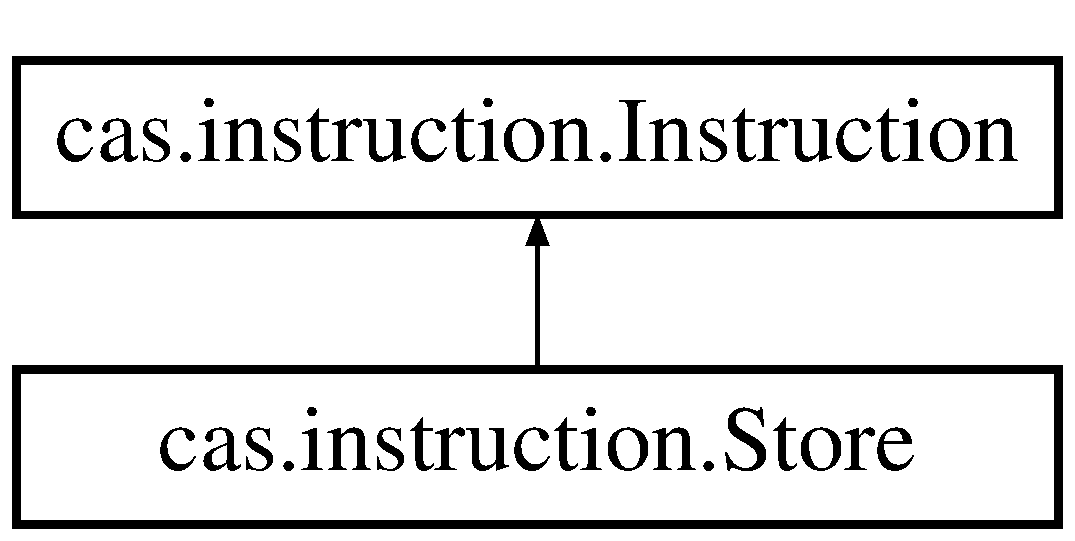
\includegraphics[height=2.000000cm]{classcas_1_1instruction_1_1_store}
\end{center}
\end{figure}
\subsection*{Public Member Functions}
\begin{DoxyCompactItemize}
\item 
\hyperlink{classcas_1_1instruction_1_1_store_a52d5abb93080a665767b0945268aeb86}{Store} ()
\item 
\hyperlink{classcas_1_1instruction_1_1_store_aa770b8c5fa1464fe2ff1f20d107038e9}{Store} (int source\-Reg, int dest\-Index)
\item 
void \hyperlink{classcas_1_1instruction_1_1_store_a6c73b7ba1d07b6af353996f2c6adb5f9}{set\-Source} (int register)
\item 
void \hyperlink{classcas_1_1instruction_1_1_store_a22b10014664b917917f05e28dec71c68}{set\-Destination} (int index)
\item 
int \hyperlink{classcas_1_1instruction_1_1_store_a0c3006d03d5a7108eaedd3d57f52424d}{get\-Source} ()
\item 
int \hyperlink{classcas_1_1instruction_1_1_store_a1373fd9c0dd7bb7ebb0f94e33587ad4a}{get\-Destination} ()
\item 
String \hyperlink{classcas_1_1instruction_1_1_store_a2b6c52613d1654df84d65e1dc1d90455}{to\-String} ()
\end{DoxyCompactItemize}


\subsection{Constructor \& Destructor Documentation}
\hypertarget{classcas_1_1instruction_1_1_store_a52d5abb93080a665767b0945268aeb86}{\index{cas\-::instruction\-::\-Store@{cas\-::instruction\-::\-Store}!Store@{Store}}
\index{Store@{Store}!cas::instruction::Store@{cas\-::instruction\-::\-Store}}
\subsubsection[{Store}]{\setlength{\rightskip}{0pt plus 5cm}cas.\-instruction.\-Store.\-Store (
\begin{DoxyParamCaption}
{}
\end{DoxyParamCaption}
)}}\label{classcas_1_1instruction_1_1_store_a52d5abb93080a665767b0945268aeb86}
\hypertarget{classcas_1_1instruction_1_1_store_aa770b8c5fa1464fe2ff1f20d107038e9}{\index{cas\-::instruction\-::\-Store@{cas\-::instruction\-::\-Store}!Store@{Store}}
\index{Store@{Store}!cas::instruction::Store@{cas\-::instruction\-::\-Store}}
\subsubsection[{Store}]{\setlength{\rightskip}{0pt plus 5cm}cas.\-instruction.\-Store.\-Store (
\begin{DoxyParamCaption}
\item[{int}]{source\-Reg, }
\item[{int}]{dest\-Index}
\end{DoxyParamCaption}
)}}\label{classcas_1_1instruction_1_1_store_aa770b8c5fa1464fe2ff1f20d107038e9}


\subsection{Member Function Documentation}
\hypertarget{classcas_1_1instruction_1_1_store_a1373fd9c0dd7bb7ebb0f94e33587ad4a}{\index{cas\-::instruction\-::\-Store@{cas\-::instruction\-::\-Store}!get\-Destination@{get\-Destination}}
\index{get\-Destination@{get\-Destination}!cas::instruction::Store@{cas\-::instruction\-::\-Store}}
\subsubsection[{get\-Destination}]{\setlength{\rightskip}{0pt plus 5cm}int cas.\-instruction.\-Store.\-get\-Destination (
\begin{DoxyParamCaption}
{}
\end{DoxyParamCaption}
)}}\label{classcas_1_1instruction_1_1_store_a1373fd9c0dd7bb7ebb0f94e33587ad4a}
\hypertarget{classcas_1_1instruction_1_1_store_a0c3006d03d5a7108eaedd3d57f52424d}{\index{cas\-::instruction\-::\-Store@{cas\-::instruction\-::\-Store}!get\-Source@{get\-Source}}
\index{get\-Source@{get\-Source}!cas::instruction::Store@{cas\-::instruction\-::\-Store}}
\subsubsection[{get\-Source}]{\setlength{\rightskip}{0pt plus 5cm}int cas.\-instruction.\-Store.\-get\-Source (
\begin{DoxyParamCaption}
{}
\end{DoxyParamCaption}
)}}\label{classcas_1_1instruction_1_1_store_a0c3006d03d5a7108eaedd3d57f52424d}
\hypertarget{classcas_1_1instruction_1_1_store_a22b10014664b917917f05e28dec71c68}{\index{cas\-::instruction\-::\-Store@{cas\-::instruction\-::\-Store}!set\-Destination@{set\-Destination}}
\index{set\-Destination@{set\-Destination}!cas::instruction::Store@{cas\-::instruction\-::\-Store}}
\subsubsection[{set\-Destination}]{\setlength{\rightskip}{0pt plus 5cm}void cas.\-instruction.\-Store.\-set\-Destination (
\begin{DoxyParamCaption}
\item[{int}]{index}
\end{DoxyParamCaption}
)}}\label{classcas_1_1instruction_1_1_store_a22b10014664b917917f05e28dec71c68}
\hypertarget{classcas_1_1instruction_1_1_store_a6c73b7ba1d07b6af353996f2c6adb5f9}{\index{cas\-::instruction\-::\-Store@{cas\-::instruction\-::\-Store}!set\-Source@{set\-Source}}
\index{set\-Source@{set\-Source}!cas::instruction::Store@{cas\-::instruction\-::\-Store}}
\subsubsection[{set\-Source}]{\setlength{\rightskip}{0pt plus 5cm}void cas.\-instruction.\-Store.\-set\-Source (
\begin{DoxyParamCaption}
\item[{int}]{register}
\end{DoxyParamCaption}
)}}\label{classcas_1_1instruction_1_1_store_a6c73b7ba1d07b6af353996f2c6adb5f9}
\hypertarget{classcas_1_1instruction_1_1_store_a2b6c52613d1654df84d65e1dc1d90455}{\index{cas\-::instruction\-::\-Store@{cas\-::instruction\-::\-Store}!to\-String@{to\-String}}
\index{to\-String@{to\-String}!cas::instruction::Store@{cas\-::instruction\-::\-Store}}
\subsubsection[{to\-String}]{\setlength{\rightskip}{0pt plus 5cm}String cas.\-instruction.\-Store.\-to\-String (
\begin{DoxyParamCaption}
{}
\end{DoxyParamCaption}
)\hspace{0.3cm}{\ttfamily [virtual]}}}\label{classcas_1_1instruction_1_1_store_a2b6c52613d1654df84d65e1dc1d90455}


Implements \hyperlink{classcas_1_1instruction_1_1_instruction_a7992edd8d79e1a4e82fb44f4c9abacf9}{cas.\-instruction.\-Instruction}.



The documentation for this class was generated from the following file\-:\begin{DoxyCompactItemize}
\item 
cas/instruction/\hyperlink{_store_8java}{Store.\-java}\end{DoxyCompactItemize}

\hypertarget{classcas_1_1instruction_1_1_store_in}{\section{cas.\-instruction.\-Store\-In Class Reference}
\label{classcas_1_1instruction_1_1_store_in}\index{cas.\-instruction.\-Store\-In@{cas.\-instruction.\-Store\-In}}
}
Inheritance diagram for cas.\-instruction.\-Store\-In\-:\begin{figure}[H]
\begin{center}
\leavevmode
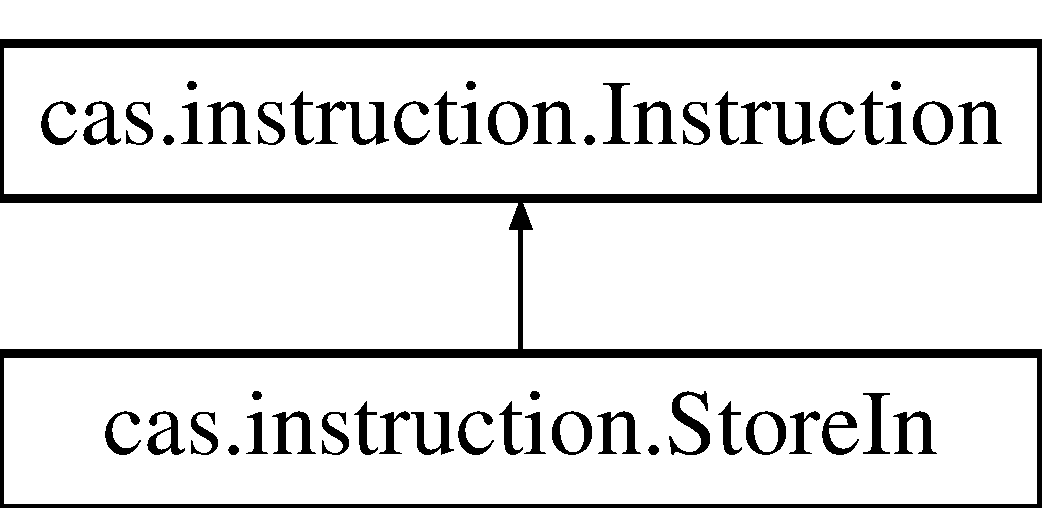
\includegraphics[height=2.000000cm]{classcas_1_1instruction_1_1_store_in}
\end{center}
\end{figure}
\subsection*{Public Member Functions}
\begin{DoxyCompactItemize}
\item 
\hyperlink{classcas_1_1instruction_1_1_store_in_a33150b212240aeadadb2cefec48e9aa3}{Store\-In} ()
\item 
\hyperlink{classcas_1_1instruction_1_1_store_in_aacb521308d8c5c6f54f5701910a7f20a}{Store\-In} (int source\-Reg, int dest\-Index, int offset\-Reg)
\item 
void \hyperlink{classcas_1_1instruction_1_1_store_in_a039f76bbf32ddba31b728c0cd2368b03}{set\-Source} (int register)
\item 
void \hyperlink{classcas_1_1instruction_1_1_store_in_ae8df4279ebed52721b5889dc3c3d9791}{set\-Offset} (int register)
\item 
void \hyperlink{classcas_1_1instruction_1_1_store_in_ae10bf3c8afc70513590d8ec97b2637bf}{set\-Destination} (int index)
\item 
int \hyperlink{classcas_1_1instruction_1_1_store_in_a052ff4369733454bd958c21baa120557}{source} ()
\item 
int \hyperlink{classcas_1_1instruction_1_1_store_in_a49f95a6de0300a080396e14561eb1b21}{destination} ()
\item 
int \hyperlink{classcas_1_1instruction_1_1_store_in_a95c4870dec04b14217758086eb7e836a}{offset} ()
\item 
String \hyperlink{classcas_1_1instruction_1_1_store_in_aed1e070aa72b5f7ec9a11a07e4488d74}{to\-String} ()
\end{DoxyCompactItemize}


\subsection{Constructor \& Destructor Documentation}
\hypertarget{classcas_1_1instruction_1_1_store_in_a33150b212240aeadadb2cefec48e9aa3}{\index{cas\-::instruction\-::\-Store\-In@{cas\-::instruction\-::\-Store\-In}!Store\-In@{Store\-In}}
\index{Store\-In@{Store\-In}!cas::instruction::StoreIn@{cas\-::instruction\-::\-Store\-In}}
\subsubsection[{Store\-In}]{\setlength{\rightskip}{0pt plus 5cm}cas.\-instruction.\-Store\-In.\-Store\-In (
\begin{DoxyParamCaption}
{}
\end{DoxyParamCaption}
)}}\label{classcas_1_1instruction_1_1_store_in_a33150b212240aeadadb2cefec48e9aa3}
\hypertarget{classcas_1_1instruction_1_1_store_in_aacb521308d8c5c6f54f5701910a7f20a}{\index{cas\-::instruction\-::\-Store\-In@{cas\-::instruction\-::\-Store\-In}!Store\-In@{Store\-In}}
\index{Store\-In@{Store\-In}!cas::instruction::StoreIn@{cas\-::instruction\-::\-Store\-In}}
\subsubsection[{Store\-In}]{\setlength{\rightskip}{0pt plus 5cm}cas.\-instruction.\-Store\-In.\-Store\-In (
\begin{DoxyParamCaption}
\item[{int}]{source\-Reg, }
\item[{int}]{dest\-Index, }
\item[{int}]{offset\-Reg}
\end{DoxyParamCaption}
)}}\label{classcas_1_1instruction_1_1_store_in_aacb521308d8c5c6f54f5701910a7f20a}


\subsection{Member Function Documentation}
\hypertarget{classcas_1_1instruction_1_1_store_in_a49f95a6de0300a080396e14561eb1b21}{\index{cas\-::instruction\-::\-Store\-In@{cas\-::instruction\-::\-Store\-In}!destination@{destination}}
\index{destination@{destination}!cas::instruction::StoreIn@{cas\-::instruction\-::\-Store\-In}}
\subsubsection[{destination}]{\setlength{\rightskip}{0pt plus 5cm}int cas.\-instruction.\-Store\-In.\-destination (
\begin{DoxyParamCaption}
{}
\end{DoxyParamCaption}
)}}\label{classcas_1_1instruction_1_1_store_in_a49f95a6de0300a080396e14561eb1b21}
\hypertarget{classcas_1_1instruction_1_1_store_in_a95c4870dec04b14217758086eb7e836a}{\index{cas\-::instruction\-::\-Store\-In@{cas\-::instruction\-::\-Store\-In}!offset@{offset}}
\index{offset@{offset}!cas::instruction::StoreIn@{cas\-::instruction\-::\-Store\-In}}
\subsubsection[{offset}]{\setlength{\rightskip}{0pt plus 5cm}int cas.\-instruction.\-Store\-In.\-offset (
\begin{DoxyParamCaption}
{}
\end{DoxyParamCaption}
)}}\label{classcas_1_1instruction_1_1_store_in_a95c4870dec04b14217758086eb7e836a}
\hypertarget{classcas_1_1instruction_1_1_store_in_ae10bf3c8afc70513590d8ec97b2637bf}{\index{cas\-::instruction\-::\-Store\-In@{cas\-::instruction\-::\-Store\-In}!set\-Destination@{set\-Destination}}
\index{set\-Destination@{set\-Destination}!cas::instruction::StoreIn@{cas\-::instruction\-::\-Store\-In}}
\subsubsection[{set\-Destination}]{\setlength{\rightskip}{0pt plus 5cm}void cas.\-instruction.\-Store\-In.\-set\-Destination (
\begin{DoxyParamCaption}
\item[{int}]{index}
\end{DoxyParamCaption}
)}}\label{classcas_1_1instruction_1_1_store_in_ae10bf3c8afc70513590d8ec97b2637bf}
\hypertarget{classcas_1_1instruction_1_1_store_in_ae8df4279ebed52721b5889dc3c3d9791}{\index{cas\-::instruction\-::\-Store\-In@{cas\-::instruction\-::\-Store\-In}!set\-Offset@{set\-Offset}}
\index{set\-Offset@{set\-Offset}!cas::instruction::StoreIn@{cas\-::instruction\-::\-Store\-In}}
\subsubsection[{set\-Offset}]{\setlength{\rightskip}{0pt plus 5cm}void cas.\-instruction.\-Store\-In.\-set\-Offset (
\begin{DoxyParamCaption}
\item[{int}]{register}
\end{DoxyParamCaption}
)}}\label{classcas_1_1instruction_1_1_store_in_ae8df4279ebed52721b5889dc3c3d9791}
\hypertarget{classcas_1_1instruction_1_1_store_in_a039f76bbf32ddba31b728c0cd2368b03}{\index{cas\-::instruction\-::\-Store\-In@{cas\-::instruction\-::\-Store\-In}!set\-Source@{set\-Source}}
\index{set\-Source@{set\-Source}!cas::instruction::StoreIn@{cas\-::instruction\-::\-Store\-In}}
\subsubsection[{set\-Source}]{\setlength{\rightskip}{0pt plus 5cm}void cas.\-instruction.\-Store\-In.\-set\-Source (
\begin{DoxyParamCaption}
\item[{int}]{register}
\end{DoxyParamCaption}
)}}\label{classcas_1_1instruction_1_1_store_in_a039f76bbf32ddba31b728c0cd2368b03}
\hypertarget{classcas_1_1instruction_1_1_store_in_a052ff4369733454bd958c21baa120557}{\index{cas\-::instruction\-::\-Store\-In@{cas\-::instruction\-::\-Store\-In}!source@{source}}
\index{source@{source}!cas::instruction::StoreIn@{cas\-::instruction\-::\-Store\-In}}
\subsubsection[{source}]{\setlength{\rightskip}{0pt plus 5cm}int cas.\-instruction.\-Store\-In.\-source (
\begin{DoxyParamCaption}
{}
\end{DoxyParamCaption}
)}}\label{classcas_1_1instruction_1_1_store_in_a052ff4369733454bd958c21baa120557}
\hypertarget{classcas_1_1instruction_1_1_store_in_aed1e070aa72b5f7ec9a11a07e4488d74}{\index{cas\-::instruction\-::\-Store\-In@{cas\-::instruction\-::\-Store\-In}!to\-String@{to\-String}}
\index{to\-String@{to\-String}!cas::instruction::StoreIn@{cas\-::instruction\-::\-Store\-In}}
\subsubsection[{to\-String}]{\setlength{\rightskip}{0pt plus 5cm}String cas.\-instruction.\-Store\-In.\-to\-String (
\begin{DoxyParamCaption}
{}
\end{DoxyParamCaption}
)\hspace{0.3cm}{\ttfamily [virtual]}}}\label{classcas_1_1instruction_1_1_store_in_aed1e070aa72b5f7ec9a11a07e4488d74}


Implements \hyperlink{classcas_1_1instruction_1_1_instruction_a7992edd8d79e1a4e82fb44f4c9abacf9}{cas.\-instruction.\-Instruction}.



The documentation for this class was generated from the following file\-:\begin{DoxyCompactItemize}
\item 
cas/instruction/\hyperlink{_store_in_8java}{Store\-In.\-java}\end{DoxyCompactItemize}

\hypertarget{classcas_1_1parser_1_1parser__containers_1_1_symbol_stack}{\section{cas.\-parser.\-parser\-\_\-containers.\-Symbol\-Stack Class Reference}
\label{classcas_1_1parser_1_1parser__containers_1_1_symbol_stack}\index{cas.\-parser.\-parser\-\_\-containers.\-Symbol\-Stack@{cas.\-parser.\-parser\-\_\-containers.\-Symbol\-Stack}}
}
\subsection*{Public Member Functions}
\begin{DoxyCompactItemize}
\item 
\hyperlink{classcas_1_1parser_1_1parser__containers_1_1_symbol_stack_a99930d1eae7f8060cd7d03a7f1c16b89}{Symbol\-Stack} ()
\item 
int \hyperlink{classcas_1_1parser_1_1parser__containers_1_1_symbol_stack_a84827706b4ac1c4f24491197641dc52e}{push} (String name, \hyperlink{enumcas_1_1machine_1_1_virtual_machine_1_1_var_type}{Var\-Type} type)  throws Runtime\-Exception
\item 
int \hyperlink{classcas_1_1parser_1_1parser__containers_1_1_symbol_stack_a396b5cb2f1a978c1c063dadb0a4e47b7}{push} (String name, \hyperlink{enumcas_1_1machine_1_1_virtual_machine_1_1_var_type}{Var\-Type} type, int size)  throws Runtime\-Exception
\item 
void \hyperlink{classcas_1_1parser_1_1parser__containers_1_1_symbol_stack_ae23e6c6b34777b5411ab87e0a76021e8}{new\-Scope} ()
\item 
int \hyperlink{classcas_1_1parser_1_1parser__containers_1_1_symbol_stack_a15d5084fb2d228c973133dbed1bea9f6}{pop} ()
\item 
boolean \hyperlink{classcas_1_1parser_1_1parser__containers_1_1_symbol_stack_ab883f94f9381cceb66ffef719b1bc9d7}{contains} (String name)
\item 
\hyperlink{classcas_1_1parser_1_1parser__containers_1_1_label}{Label} \hyperlink{classcas_1_1parser_1_1parser__containers_1_1_symbol_stack_abeb44281cfe750d43c65e56e4312bcd9}{get\-Label} (String name)  throws Runtime\-Exception
\item 
String \hyperlink{classcas_1_1parser_1_1parser__containers_1_1_symbol_stack_ac3a5a77bda4b08d6b87f3996c6cbf687}{to\-String} ()
\end{DoxyCompactItemize}


\subsection{Constructor \& Destructor Documentation}
\hypertarget{classcas_1_1parser_1_1parser__containers_1_1_symbol_stack_a99930d1eae7f8060cd7d03a7f1c16b89}{\index{cas\-::parser\-::parser\-\_\-containers\-::\-Symbol\-Stack@{cas\-::parser\-::parser\-\_\-containers\-::\-Symbol\-Stack}!Symbol\-Stack@{Symbol\-Stack}}
\index{Symbol\-Stack@{Symbol\-Stack}!cas::parser::parser_containers::SymbolStack@{cas\-::parser\-::parser\-\_\-containers\-::\-Symbol\-Stack}}
\subsubsection[{Symbol\-Stack}]{\setlength{\rightskip}{0pt plus 5cm}cas.\-parser.\-parser\-\_\-containers.\-Symbol\-Stack.\-Symbol\-Stack (
\begin{DoxyParamCaption}
{}
\end{DoxyParamCaption}
)}}\label{classcas_1_1parser_1_1parser__containers_1_1_symbol_stack_a99930d1eae7f8060cd7d03a7f1c16b89}


\subsection{Member Function Documentation}
\hypertarget{classcas_1_1parser_1_1parser__containers_1_1_symbol_stack_ab883f94f9381cceb66ffef719b1bc9d7}{\index{cas\-::parser\-::parser\-\_\-containers\-::\-Symbol\-Stack@{cas\-::parser\-::parser\-\_\-containers\-::\-Symbol\-Stack}!contains@{contains}}
\index{contains@{contains}!cas::parser::parser_containers::SymbolStack@{cas\-::parser\-::parser\-\_\-containers\-::\-Symbol\-Stack}}
\subsubsection[{contains}]{\setlength{\rightskip}{0pt plus 5cm}boolean cas.\-parser.\-parser\-\_\-containers.\-Symbol\-Stack.\-contains (
\begin{DoxyParamCaption}
\item[{String}]{name}
\end{DoxyParamCaption}
)}}\label{classcas_1_1parser_1_1parser__containers_1_1_symbol_stack_ab883f94f9381cceb66ffef719b1bc9d7}
\hypertarget{classcas_1_1parser_1_1parser__containers_1_1_symbol_stack_abeb44281cfe750d43c65e56e4312bcd9}{\index{cas\-::parser\-::parser\-\_\-containers\-::\-Symbol\-Stack@{cas\-::parser\-::parser\-\_\-containers\-::\-Symbol\-Stack}!get\-Label@{get\-Label}}
\index{get\-Label@{get\-Label}!cas::parser::parser_containers::SymbolStack@{cas\-::parser\-::parser\-\_\-containers\-::\-Symbol\-Stack}}
\subsubsection[{get\-Label}]{\setlength{\rightskip}{0pt plus 5cm}{\bf Label} cas.\-parser.\-parser\-\_\-containers.\-Symbol\-Stack.\-get\-Label (
\begin{DoxyParamCaption}
\item[{String}]{name}
\end{DoxyParamCaption}
)  throws Runtime\-Exception}}\label{classcas_1_1parser_1_1parser__containers_1_1_symbol_stack_abeb44281cfe750d43c65e56e4312bcd9}
\hypertarget{classcas_1_1parser_1_1parser__containers_1_1_symbol_stack_ae23e6c6b34777b5411ab87e0a76021e8}{\index{cas\-::parser\-::parser\-\_\-containers\-::\-Symbol\-Stack@{cas\-::parser\-::parser\-\_\-containers\-::\-Symbol\-Stack}!new\-Scope@{new\-Scope}}
\index{new\-Scope@{new\-Scope}!cas::parser::parser_containers::SymbolStack@{cas\-::parser\-::parser\-\_\-containers\-::\-Symbol\-Stack}}
\subsubsection[{new\-Scope}]{\setlength{\rightskip}{0pt plus 5cm}void cas.\-parser.\-parser\-\_\-containers.\-Symbol\-Stack.\-new\-Scope (
\begin{DoxyParamCaption}
{}
\end{DoxyParamCaption}
)}}\label{classcas_1_1parser_1_1parser__containers_1_1_symbol_stack_ae23e6c6b34777b5411ab87e0a76021e8}
\hypertarget{classcas_1_1parser_1_1parser__containers_1_1_symbol_stack_a15d5084fb2d228c973133dbed1bea9f6}{\index{cas\-::parser\-::parser\-\_\-containers\-::\-Symbol\-Stack@{cas\-::parser\-::parser\-\_\-containers\-::\-Symbol\-Stack}!pop@{pop}}
\index{pop@{pop}!cas::parser::parser_containers::SymbolStack@{cas\-::parser\-::parser\-\_\-containers\-::\-Symbol\-Stack}}
\subsubsection[{pop}]{\setlength{\rightskip}{0pt plus 5cm}int cas.\-parser.\-parser\-\_\-containers.\-Symbol\-Stack.\-pop (
\begin{DoxyParamCaption}
{}
\end{DoxyParamCaption}
)}}\label{classcas_1_1parser_1_1parser__containers_1_1_symbol_stack_a15d5084fb2d228c973133dbed1bea9f6}
\hypertarget{classcas_1_1parser_1_1parser__containers_1_1_symbol_stack_a84827706b4ac1c4f24491197641dc52e}{\index{cas\-::parser\-::parser\-\_\-containers\-::\-Symbol\-Stack@{cas\-::parser\-::parser\-\_\-containers\-::\-Symbol\-Stack}!push@{push}}
\index{push@{push}!cas::parser::parser_containers::SymbolStack@{cas\-::parser\-::parser\-\_\-containers\-::\-Symbol\-Stack}}
\subsubsection[{push}]{\setlength{\rightskip}{0pt plus 5cm}int cas.\-parser.\-parser\-\_\-containers.\-Symbol\-Stack.\-push (
\begin{DoxyParamCaption}
\item[{String}]{name, }
\item[{{\bf Var\-Type}}]{type}
\end{DoxyParamCaption}
)  throws Runtime\-Exception}}\label{classcas_1_1parser_1_1parser__containers_1_1_symbol_stack_a84827706b4ac1c4f24491197641dc52e}
\hypertarget{classcas_1_1parser_1_1parser__containers_1_1_symbol_stack_a396b5cb2f1a978c1c063dadb0a4e47b7}{\index{cas\-::parser\-::parser\-\_\-containers\-::\-Symbol\-Stack@{cas\-::parser\-::parser\-\_\-containers\-::\-Symbol\-Stack}!push@{push}}
\index{push@{push}!cas::parser::parser_containers::SymbolStack@{cas\-::parser\-::parser\-\_\-containers\-::\-Symbol\-Stack}}
\subsubsection[{push}]{\setlength{\rightskip}{0pt plus 5cm}int cas.\-parser.\-parser\-\_\-containers.\-Symbol\-Stack.\-push (
\begin{DoxyParamCaption}
\item[{String}]{name, }
\item[{{\bf Var\-Type}}]{type, }
\item[{int}]{size}
\end{DoxyParamCaption}
)  throws Runtime\-Exception}}\label{classcas_1_1parser_1_1parser__containers_1_1_symbol_stack_a396b5cb2f1a978c1c063dadb0a4e47b7}
\hypertarget{classcas_1_1parser_1_1parser__containers_1_1_symbol_stack_ac3a5a77bda4b08d6b87f3996c6cbf687}{\index{cas\-::parser\-::parser\-\_\-containers\-::\-Symbol\-Stack@{cas\-::parser\-::parser\-\_\-containers\-::\-Symbol\-Stack}!to\-String@{to\-String}}
\index{to\-String@{to\-String}!cas::parser::parser_containers::SymbolStack@{cas\-::parser\-::parser\-\_\-containers\-::\-Symbol\-Stack}}
\subsubsection[{to\-String}]{\setlength{\rightskip}{0pt plus 5cm}String cas.\-parser.\-parser\-\_\-containers.\-Symbol\-Stack.\-to\-String (
\begin{DoxyParamCaption}
{}
\end{DoxyParamCaption}
)}}\label{classcas_1_1parser_1_1parser__containers_1_1_symbol_stack_ac3a5a77bda4b08d6b87f3996c6cbf687}


The documentation for this class was generated from the following file\-:\begin{DoxyCompactItemize}
\item 
cas/parser/parser\-\_\-containers/\hyperlink{_symbol_stack_8java}{Symbol\-Stack.\-java}\end{DoxyCompactItemize}

\hypertarget{classtools_1_1_tools}{\section{tools.\-Tools Class Reference}
\label{classtools_1_1_tools}\index{tools.\-Tools@{tools.\-Tools}}
}
\subsection*{Static Public Member Functions}
\begin{DoxyCompactItemize}
\item 
static int\mbox{[}$\,$\mbox{]} \hyperlink{classtools_1_1_tools_a621ac19b273c9133ccb49f88b5471c57}{deci\-To\-Base} (int number, int base, int digits)
\item 
static int\mbox{[}$\,$\mbox{]} \hyperlink{classtools_1_1_tools_aba05ac830f156b291a0bf96b37a69283}{deci\-To\-Base} (int number, int base)
\item 
static int \hyperlink{classtools_1_1_tools_aa434ed3be898880a6c173cef2b5993f0}{base\-To\-Deci} (int\mbox{[}$\,$\mbox{]} number, int base)
\item 
static String \hyperlink{classtools_1_1_tools_ab0e03a005710d3634755829037e9e8f4}{to\-Binary\-String} (int number, int digits)
\item 
static String \hyperlink{classtools_1_1_tools_a516db6be7076f6f06b28097571fe4d86}{to\-Hex\-String} (int number, int digits)
\item 
static short \hyperlink{classtools_1_1_tools_addca99979e298d0344eebc63c472d321}{hex\-To\-Short} (String hex, int max\-Digits)  throws Input\-Mismatch\-Exception 
\end{DoxyCompactItemize}


\subsection{Member Function Documentation}
\hypertarget{classtools_1_1_tools_aa434ed3be898880a6c173cef2b5993f0}{\index{tools\-::\-Tools@{tools\-::\-Tools}!base\-To\-Deci@{base\-To\-Deci}}
\index{base\-To\-Deci@{base\-To\-Deci}!tools::Tools@{tools\-::\-Tools}}
\subsubsection[{base\-To\-Deci}]{\setlength{\rightskip}{0pt plus 5cm}static int tools.\-Tools.\-base\-To\-Deci (
\begin{DoxyParamCaption}
\item[{int\mbox{[}$\,$\mbox{]}}]{number, }
\item[{int}]{base}
\end{DoxyParamCaption}
)\hspace{0.3cm}{\ttfamily [static]}}}\label{classtools_1_1_tools_aa434ed3be898880a6c173cef2b5993f0}
\hypertarget{classtools_1_1_tools_a621ac19b273c9133ccb49f88b5471c57}{\index{tools\-::\-Tools@{tools\-::\-Tools}!deci\-To\-Base@{deci\-To\-Base}}
\index{deci\-To\-Base@{deci\-To\-Base}!tools::Tools@{tools\-::\-Tools}}
\subsubsection[{deci\-To\-Base}]{\setlength{\rightskip}{0pt plus 5cm}static int \mbox{[}$\,$\mbox{]} tools.\-Tools.\-deci\-To\-Base (
\begin{DoxyParamCaption}
\item[{int}]{number, }
\item[{int}]{base, }
\item[{int}]{digits}
\end{DoxyParamCaption}
)\hspace{0.3cm}{\ttfamily [static]}}}\label{classtools_1_1_tools_a621ac19b273c9133ccb49f88b5471c57}
\hypertarget{classtools_1_1_tools_aba05ac830f156b291a0bf96b37a69283}{\index{tools\-::\-Tools@{tools\-::\-Tools}!deci\-To\-Base@{deci\-To\-Base}}
\index{deci\-To\-Base@{deci\-To\-Base}!tools::Tools@{tools\-::\-Tools}}
\subsubsection[{deci\-To\-Base}]{\setlength{\rightskip}{0pt plus 5cm}static int \mbox{[}$\,$\mbox{]} tools.\-Tools.\-deci\-To\-Base (
\begin{DoxyParamCaption}
\item[{int}]{number, }
\item[{int}]{base}
\end{DoxyParamCaption}
)\hspace{0.3cm}{\ttfamily [static]}}}\label{classtools_1_1_tools_aba05ac830f156b291a0bf96b37a69283}
\hypertarget{classtools_1_1_tools_addca99979e298d0344eebc63c472d321}{\index{tools\-::\-Tools@{tools\-::\-Tools}!hex\-To\-Short@{hex\-To\-Short}}
\index{hex\-To\-Short@{hex\-To\-Short}!tools::Tools@{tools\-::\-Tools}}
\subsubsection[{hex\-To\-Short}]{\setlength{\rightskip}{0pt plus 5cm}static short tools.\-Tools.\-hex\-To\-Short (
\begin{DoxyParamCaption}
\item[{String}]{hex, }
\item[{int}]{max\-Digits}
\end{DoxyParamCaption}
)  throws Input\-Mismatch\-Exception \hspace{0.3cm}{\ttfamily [static]}}}\label{classtools_1_1_tools_addca99979e298d0344eebc63c472d321}
\hypertarget{classtools_1_1_tools_ab0e03a005710d3634755829037e9e8f4}{\index{tools\-::\-Tools@{tools\-::\-Tools}!to\-Binary\-String@{to\-Binary\-String}}
\index{to\-Binary\-String@{to\-Binary\-String}!tools::Tools@{tools\-::\-Tools}}
\subsubsection[{to\-Binary\-String}]{\setlength{\rightskip}{0pt plus 5cm}static String tools.\-Tools.\-to\-Binary\-String (
\begin{DoxyParamCaption}
\item[{int}]{number, }
\item[{int}]{digits}
\end{DoxyParamCaption}
)\hspace{0.3cm}{\ttfamily [static]}}}\label{classtools_1_1_tools_ab0e03a005710d3634755829037e9e8f4}
\hypertarget{classtools_1_1_tools_a516db6be7076f6f06b28097571fe4d86}{\index{tools\-::\-Tools@{tools\-::\-Tools}!to\-Hex\-String@{to\-Hex\-String}}
\index{to\-Hex\-String@{to\-Hex\-String}!tools::Tools@{tools\-::\-Tools}}
\subsubsection[{to\-Hex\-String}]{\setlength{\rightskip}{0pt plus 5cm}static String tools.\-Tools.\-to\-Hex\-String (
\begin{DoxyParamCaption}
\item[{int}]{number, }
\item[{int}]{digits}
\end{DoxyParamCaption}
)\hspace{0.3cm}{\ttfamily [static]}}}\label{classtools_1_1_tools_a516db6be7076f6f06b28097571fe4d86}


The documentation for this class was generated from the following file\-:\begin{DoxyCompactItemize}
\item 
tools/\hyperlink{_tools_8java}{Tools.\-java}\end{DoxyCompactItemize}

\hypertarget{enumcas_1_1machine_1_1_virtual_machine_1_1_var_type}{\section{cas.\-machine.\-Virtual\-Machine.\-Var\-Type Enum Reference}
\label{enumcas_1_1machine_1_1_virtual_machine_1_1_var_type}\index{cas.\-machine.\-Virtual\-Machine.\-Var\-Type@{cas.\-machine.\-Virtual\-Machine.\-Var\-Type}}
}
\subsection*{Public Attributes}
\begin{DoxyCompactItemize}
\item 
\hyperlink{enumcas_1_1machine_1_1_virtual_machine_1_1_var_type_a5d8d3d6bae08973794306dc86eaa60e4}{I\-N\-T}
\item 
\hyperlink{enumcas_1_1machine_1_1_virtual_machine_1_1_var_type_a31daa7c97eb5e17ff6d88702c2022739}{R\-E\-A\-L}
\item 
\hyperlink{enumcas_1_1machine_1_1_virtual_machine_1_1_var_type_a14d1551cc662f8f41c5d8756391cbc27}{B\-O\-O\-L\-E}
\end{DoxyCompactItemize}


\subsection{Member Data Documentation}
\hypertarget{enumcas_1_1machine_1_1_virtual_machine_1_1_var_type_a14d1551cc662f8f41c5d8756391cbc27}{\index{cas\-::machine\-::\-Virtual\-Machine\-::\-Var\-Type@{cas\-::machine\-::\-Virtual\-Machine\-::\-Var\-Type}!B\-O\-O\-L\-E@{B\-O\-O\-L\-E}}
\index{B\-O\-O\-L\-E@{B\-O\-O\-L\-E}!cas::machine::VirtualMachine::VarType@{cas\-::machine\-::\-Virtual\-Machine\-::\-Var\-Type}}
\subsubsection[{B\-O\-O\-L\-E}]{\setlength{\rightskip}{0pt plus 5cm}cas.\-machine.\-Virtual\-Machine.\-Var\-Type.\-B\-O\-O\-L\-E}}\label{enumcas_1_1machine_1_1_virtual_machine_1_1_var_type_a14d1551cc662f8f41c5d8756391cbc27}
\hypertarget{enumcas_1_1machine_1_1_virtual_machine_1_1_var_type_a5d8d3d6bae08973794306dc86eaa60e4}{\index{cas\-::machine\-::\-Virtual\-Machine\-::\-Var\-Type@{cas\-::machine\-::\-Virtual\-Machine\-::\-Var\-Type}!I\-N\-T@{I\-N\-T}}
\index{I\-N\-T@{I\-N\-T}!cas::machine::VirtualMachine::VarType@{cas\-::machine\-::\-Virtual\-Machine\-::\-Var\-Type}}
\subsubsection[{I\-N\-T}]{\setlength{\rightskip}{0pt plus 5cm}cas.\-machine.\-Virtual\-Machine.\-Var\-Type.\-I\-N\-T}}\label{enumcas_1_1machine_1_1_virtual_machine_1_1_var_type_a5d8d3d6bae08973794306dc86eaa60e4}
\hypertarget{enumcas_1_1machine_1_1_virtual_machine_1_1_var_type_a31daa7c97eb5e17ff6d88702c2022739}{\index{cas\-::machine\-::\-Virtual\-Machine\-::\-Var\-Type@{cas\-::machine\-::\-Virtual\-Machine\-::\-Var\-Type}!R\-E\-A\-L@{R\-E\-A\-L}}
\index{R\-E\-A\-L@{R\-E\-A\-L}!cas::machine::VirtualMachine::VarType@{cas\-::machine\-::\-Virtual\-Machine\-::\-Var\-Type}}
\subsubsection[{R\-E\-A\-L}]{\setlength{\rightskip}{0pt plus 5cm}cas.\-machine.\-Virtual\-Machine.\-Var\-Type.\-R\-E\-A\-L}}\label{enumcas_1_1machine_1_1_virtual_machine_1_1_var_type_a31daa7c97eb5e17ff6d88702c2022739}


The documentation for this enum was generated from the following file\-:\begin{DoxyCompactItemize}
\item 
cas/machine/\hyperlink{_virtual_machine_8java}{Virtual\-Machine.\-java}\end{DoxyCompactItemize}

\hypertarget{classcas_1_1machine_1_1_virtual_machine}{\section{cas.\-machine.\-Virtual\-Machine Class Reference}
\label{classcas_1_1machine_1_1_virtual_machine}\index{cas.\-machine.\-Virtual\-Machine@{cas.\-machine.\-Virtual\-Machine}}
}
\subsection*{Classes}
\begin{DoxyCompactItemize}
\item 
enum \hyperlink{enumcas_1_1machine_1_1_virtual_machine_1_1_var_type}{Var\-Type}
\end{DoxyCompactItemize}
\subsection*{Public Member Functions}
\begin{DoxyCompactItemize}
\item 
\hyperlink{classcas_1_1machine_1_1_virtual_machine_ac8d09a9686872aed0c9b7782446819f2}{Virtual\-Machine} ()
\item 
\hyperlink{classcas_1_1machine_1_1_virtual_machine_acbbcc8ca352e51129a43c9a3a3718754}{Virtual\-Machine} (\hyperlink{classcas_1_1parser_1_1parser__containers_1_1_code_list}{Code\-List} list)
\item 
\hyperlink{classcas_1_1machine_1_1_virtual_machine_a1eb1370751ba6246de430051e075b3b1}{Virtual\-Machine} (Instruction instructions\mbox{[}$\,$\mbox{]})
\item 
Object \hyperlink{classcas_1_1machine_1_1_virtual_machine_a0e43df1c0a5832701e9c8a777844a499}{execute} ()
\item 
Object \hyperlink{classcas_1_1machine_1_1_virtual_machine_a3b1fd3da1be7d57711197416f3ef7b67}{step} ()  throws Runtime\-Exception 
\item 
void \hyperlink{classcas_1_1machine_1_1_virtual_machine_a4cc756bb1c0b6e5a1b69c1f819289685}{insert\-Memory} (int i, Object element)
\item 
void \hyperlink{classcas_1_1machine_1_1_virtual_machine_afc4f326f23930f945a704b35f819a21b}{push\-Memory} (Object element)
\item 
void \hyperlink{classcas_1_1machine_1_1_virtual_machine_a195dc7502075e8feaa1998f99230916e}{reset} ()
\end{DoxyCompactItemize}


\subsection{Constructor \& Destructor Documentation}
\hypertarget{classcas_1_1machine_1_1_virtual_machine_ac8d09a9686872aed0c9b7782446819f2}{\index{cas\-::machine\-::\-Virtual\-Machine@{cas\-::machine\-::\-Virtual\-Machine}!Virtual\-Machine@{Virtual\-Machine}}
\index{Virtual\-Machine@{Virtual\-Machine}!cas::machine::VirtualMachine@{cas\-::machine\-::\-Virtual\-Machine}}
\subsubsection[{Virtual\-Machine}]{\setlength{\rightskip}{0pt plus 5cm}cas.\-machine.\-Virtual\-Machine.\-Virtual\-Machine (
\begin{DoxyParamCaption}
{}
\end{DoxyParamCaption}
)}}\label{classcas_1_1machine_1_1_virtual_machine_ac8d09a9686872aed0c9b7782446819f2}
\hypertarget{classcas_1_1machine_1_1_virtual_machine_acbbcc8ca352e51129a43c9a3a3718754}{\index{cas\-::machine\-::\-Virtual\-Machine@{cas\-::machine\-::\-Virtual\-Machine}!Virtual\-Machine@{Virtual\-Machine}}
\index{Virtual\-Machine@{Virtual\-Machine}!cas::machine::VirtualMachine@{cas\-::machine\-::\-Virtual\-Machine}}
\subsubsection[{Virtual\-Machine}]{\setlength{\rightskip}{0pt plus 5cm}cas.\-machine.\-Virtual\-Machine.\-Virtual\-Machine (
\begin{DoxyParamCaption}
\item[{{\bf Code\-List}}]{list}
\end{DoxyParamCaption}
)}}\label{classcas_1_1machine_1_1_virtual_machine_acbbcc8ca352e51129a43c9a3a3718754}
\hypertarget{classcas_1_1machine_1_1_virtual_machine_a1eb1370751ba6246de430051e075b3b1}{\index{cas\-::machine\-::\-Virtual\-Machine@{cas\-::machine\-::\-Virtual\-Machine}!Virtual\-Machine@{Virtual\-Machine}}
\index{Virtual\-Machine@{Virtual\-Machine}!cas::machine::VirtualMachine@{cas\-::machine\-::\-Virtual\-Machine}}
\subsubsection[{Virtual\-Machine}]{\setlength{\rightskip}{0pt plus 5cm}cas.\-machine.\-Virtual\-Machine.\-Virtual\-Machine (
\begin{DoxyParamCaption}
\item[{Instruction}]{instructions\mbox{[}$\,$\mbox{]}}
\end{DoxyParamCaption}
)}}\label{classcas_1_1machine_1_1_virtual_machine_a1eb1370751ba6246de430051e075b3b1}


\subsection{Member Function Documentation}
\hypertarget{classcas_1_1machine_1_1_virtual_machine_a0e43df1c0a5832701e9c8a777844a499}{\index{cas\-::machine\-::\-Virtual\-Machine@{cas\-::machine\-::\-Virtual\-Machine}!execute@{execute}}
\index{execute@{execute}!cas::machine::VirtualMachine@{cas\-::machine\-::\-Virtual\-Machine}}
\subsubsection[{execute}]{\setlength{\rightskip}{0pt plus 5cm}Object cas.\-machine.\-Virtual\-Machine.\-execute (
\begin{DoxyParamCaption}
{}
\end{DoxyParamCaption}
)}}\label{classcas_1_1machine_1_1_virtual_machine_a0e43df1c0a5832701e9c8a777844a499}
\hypertarget{classcas_1_1machine_1_1_virtual_machine_a4cc756bb1c0b6e5a1b69c1f819289685}{\index{cas\-::machine\-::\-Virtual\-Machine@{cas\-::machine\-::\-Virtual\-Machine}!insert\-Memory@{insert\-Memory}}
\index{insert\-Memory@{insert\-Memory}!cas::machine::VirtualMachine@{cas\-::machine\-::\-Virtual\-Machine}}
\subsubsection[{insert\-Memory}]{\setlength{\rightskip}{0pt plus 5cm}void cas.\-machine.\-Virtual\-Machine.\-insert\-Memory (
\begin{DoxyParamCaption}
\item[{int}]{i, }
\item[{Object}]{element}
\end{DoxyParamCaption}
)}}\label{classcas_1_1machine_1_1_virtual_machine_a4cc756bb1c0b6e5a1b69c1f819289685}
\hypertarget{classcas_1_1machine_1_1_virtual_machine_afc4f326f23930f945a704b35f819a21b}{\index{cas\-::machine\-::\-Virtual\-Machine@{cas\-::machine\-::\-Virtual\-Machine}!push\-Memory@{push\-Memory}}
\index{push\-Memory@{push\-Memory}!cas::machine::VirtualMachine@{cas\-::machine\-::\-Virtual\-Machine}}
\subsubsection[{push\-Memory}]{\setlength{\rightskip}{0pt plus 5cm}void cas.\-machine.\-Virtual\-Machine.\-push\-Memory (
\begin{DoxyParamCaption}
\item[{Object}]{element}
\end{DoxyParamCaption}
)}}\label{classcas_1_1machine_1_1_virtual_machine_afc4f326f23930f945a704b35f819a21b}
\hypertarget{classcas_1_1machine_1_1_virtual_machine_a195dc7502075e8feaa1998f99230916e}{\index{cas\-::machine\-::\-Virtual\-Machine@{cas\-::machine\-::\-Virtual\-Machine}!reset@{reset}}
\index{reset@{reset}!cas::machine::VirtualMachine@{cas\-::machine\-::\-Virtual\-Machine}}
\subsubsection[{reset}]{\setlength{\rightskip}{0pt plus 5cm}void cas.\-machine.\-Virtual\-Machine.\-reset (
\begin{DoxyParamCaption}
{}
\end{DoxyParamCaption}
)}}\label{classcas_1_1machine_1_1_virtual_machine_a195dc7502075e8feaa1998f99230916e}
\hypertarget{classcas_1_1machine_1_1_virtual_machine_a3b1fd3da1be7d57711197416f3ef7b67}{\index{cas\-::machine\-::\-Virtual\-Machine@{cas\-::machine\-::\-Virtual\-Machine}!step@{step}}
\index{step@{step}!cas::machine::VirtualMachine@{cas\-::machine\-::\-Virtual\-Machine}}
\subsubsection[{step}]{\setlength{\rightskip}{0pt plus 5cm}Object cas.\-machine.\-Virtual\-Machine.\-step (
\begin{DoxyParamCaption}
{}
\end{DoxyParamCaption}
)  throws Runtime\-Exception }}\label{classcas_1_1machine_1_1_virtual_machine_a3b1fd3da1be7d57711197416f3ef7b67}


The documentation for this class was generated from the following file\-:\begin{DoxyCompactItemize}
\item 
cas/machine/\hyperlink{_virtual_machine_8java}{Virtual\-Machine.\-java}\end{DoxyCompactItemize}

\chapter{File Documentation}
\hypertarget{_automata_8java}{\section{cas/automata/\-Automata.java File Reference}
\label{_automata_8java}\index{cas/automata/\-Automata.\-java@{cas/automata/\-Automata.\-java}}
}
\subsection*{Classes}
\begin{DoxyCompactItemize}
\item 
class \hyperlink{classcas_1_1automata_1_1_automata}{cas.\-automata.\-Automata}
\end{DoxyCompactItemize}
\subsection*{Packages}
\begin{DoxyCompactItemize}
\item 
package \hyperlink{namespacecas_1_1automata}{cas.\-automata}
\end{DoxyCompactItemize}

\hypertarget{_allocate_array_8java}{\section{cas/instruction/\-Allocate\-Array.java File Reference}
\label{_allocate_array_8java}\index{cas/instruction/\-Allocate\-Array.\-java@{cas/instruction/\-Allocate\-Array.\-java}}
}
\subsection*{Classes}
\begin{DoxyCompactItemize}
\item 
class \hyperlink{classcas_1_1instruction_1_1_allocate_array}{cas.\-instruction.\-Allocate\-Array}
\end{DoxyCompactItemize}
\subsection*{Packages}
\begin{DoxyCompactItemize}
\item 
package \hyperlink{namespacecas_1_1instruction}{cas.\-instruction}
\end{DoxyCompactItemize}

\hypertarget{_break_8java}{\section{cas/instruction/\-Break.java File Reference}
\label{_break_8java}\index{cas/instruction/\-Break.\-java@{cas/instruction/\-Break.\-java}}
}
\subsection*{Classes}
\begin{DoxyCompactItemize}
\item 
class \hyperlink{classcas_1_1instruction_1_1_break}{cas.\-instruction.\-Break}
\item 
enum \hyperlink{enumcas_1_1instruction_1_1_break_1_1_condition}{cas.\-instruction.\-Break.\-Condition}
\end{DoxyCompactItemize}
\subsection*{Packages}
\begin{DoxyCompactItemize}
\item 
package \hyperlink{namespacecas_1_1instruction}{cas.\-instruction}
\end{DoxyCompactItemize}

\hypertarget{_halt_return_8java}{\section{cas/instruction/\-Halt\-Return.java File Reference}
\label{_halt_return_8java}\index{cas/instruction/\-Halt\-Return.\-java@{cas/instruction/\-Halt\-Return.\-java}}
}
\subsection*{Classes}
\begin{DoxyCompactItemize}
\item 
class \hyperlink{classcas_1_1instruction_1_1_halt_return}{cas.\-instruction.\-Halt\-Return}
\end{DoxyCompactItemize}
\subsection*{Packages}
\begin{DoxyCompactItemize}
\item 
package \hyperlink{namespacecas_1_1instruction}{cas.\-instruction}
\end{DoxyCompactItemize}

\hypertarget{_instruction_8java}{\section{cas/instruction/\-Instruction.java File Reference}
\label{_instruction_8java}\index{cas/instruction/\-Instruction.\-java@{cas/instruction/\-Instruction.\-java}}
}
\subsection*{Classes}
\begin{DoxyCompactItemize}
\item 
class \hyperlink{classcas_1_1instruction_1_1_instruction}{cas.\-instruction.\-Instruction}
\item 
enum \hyperlink{enumcas_1_1instruction_1_1_instruction_1_1_instruction_type}{cas.\-instruction.\-Instruction.\-Instruction\-Type}
\end{DoxyCompactItemize}
\subsection*{Packages}
\begin{DoxyCompactItemize}
\item 
package \hyperlink{namespacecas_1_1instruction}{cas.\-instruction}
\end{DoxyCompactItemize}

\hypertarget{_jump_8java}{\section{cas/instruction/\-Jump.java File Reference}
\label{_jump_8java}\index{cas/instruction/\-Jump.\-java@{cas/instruction/\-Jump.\-java}}
}
\subsection*{Classes}
\begin{DoxyCompactItemize}
\item 
class \hyperlink{classcas_1_1instruction_1_1_jump}{cas.\-instruction.\-Jump}
\end{DoxyCompactItemize}
\subsection*{Packages}
\begin{DoxyCompactItemize}
\item 
package \hyperlink{namespacecas_1_1instruction}{cas.\-instruction}
\end{DoxyCompactItemize}

\hypertarget{_load_8java}{\section{cas/instruction/\-Load.java File Reference}
\label{_load_8java}\index{cas/instruction/\-Load.\-java@{cas/instruction/\-Load.\-java}}
}
\subsection*{Classes}
\begin{DoxyCompactItemize}
\item 
class \hyperlink{classcas_1_1instruction_1_1_load}{cas.\-instruction.\-Load}
\end{DoxyCompactItemize}
\subsection*{Packages}
\begin{DoxyCompactItemize}
\item 
package \hyperlink{namespacecas_1_1instruction}{cas.\-instruction}
\end{DoxyCompactItemize}

\hypertarget{_load_immediate_8java}{\section{cas/instruction/\-Load\-Immediate.java File Reference}
\label{_load_immediate_8java}\index{cas/instruction/\-Load\-Immediate.\-java@{cas/instruction/\-Load\-Immediate.\-java}}
}
\subsection*{Classes}
\begin{DoxyCompactItemize}
\item 
class \hyperlink{classcas_1_1instruction_1_1_load_immediate}{cas.\-instruction.\-Load\-Immediate}
\end{DoxyCompactItemize}
\subsection*{Packages}
\begin{DoxyCompactItemize}
\item 
package \hyperlink{namespacecas_1_1instruction}{cas.\-instruction}
\end{DoxyCompactItemize}

\hypertarget{_load_in_8java}{\section{cas/instruction/\-Load\-In.java File Reference}
\label{_load_in_8java}\index{cas/instruction/\-Load\-In.\-java@{cas/instruction/\-Load\-In.\-java}}
}
\subsection*{Classes}
\begin{DoxyCompactItemize}
\item 
class \hyperlink{classcas_1_1instruction_1_1_load_in}{cas.\-instruction.\-Load\-In}
\end{DoxyCompactItemize}
\subsection*{Packages}
\begin{DoxyCompactItemize}
\item 
package \hyperlink{namespacecas_1_1instruction}{cas.\-instruction}
\end{DoxyCompactItemize}

\hypertarget{_operator_8java}{\section{cas/instruction/\-Operator.java File Reference}
\label{_operator_8java}\index{cas/instruction/\-Operator.\-java@{cas/instruction/\-Operator.\-java}}
}
\subsection*{Classes}
\begin{DoxyCompactItemize}
\item 
class \hyperlink{classcas_1_1instruction_1_1_operator}{cas.\-instruction.\-Operator}
\item 
enum \hyperlink{enumcas_1_1instruction_1_1_operator_1_1_operation}{cas.\-instruction.\-Operator.\-Operation}
\end{DoxyCompactItemize}
\subsection*{Packages}
\begin{DoxyCompactItemize}
\item 
package \hyperlink{namespacecas_1_1instruction}{cas.\-instruction}
\end{DoxyCompactItemize}

\hypertarget{_store_8java}{\section{cas/instruction/\-Store.java File Reference}
\label{_store_8java}\index{cas/instruction/\-Store.\-java@{cas/instruction/\-Store.\-java}}
}
\subsection*{Classes}
\begin{DoxyCompactItemize}
\item 
class \hyperlink{classcas_1_1instruction_1_1_store}{cas.\-instruction.\-Store}
\end{DoxyCompactItemize}
\subsection*{Packages}
\begin{DoxyCompactItemize}
\item 
package \hyperlink{namespacecas_1_1instruction}{cas.\-instruction}
\end{DoxyCompactItemize}

\hypertarget{_store_in_8java}{\section{cas/instruction/\-Store\-In.java File Reference}
\label{_store_in_8java}\index{cas/instruction/\-Store\-In.\-java@{cas/instruction/\-Store\-In.\-java}}
}
\subsection*{Classes}
\begin{DoxyCompactItemize}
\item 
class \hyperlink{classcas_1_1instruction_1_1_store_in}{cas.\-instruction.\-Store\-In}
\end{DoxyCompactItemize}
\subsection*{Packages}
\begin{DoxyCompactItemize}
\item 
package \hyperlink{namespacecas_1_1instruction}{cas.\-instruction}
\end{DoxyCompactItemize}

\hypertarget{_virtual_machine_8java}{\section{cas/machine/\-Virtual\-Machine.java File Reference}
\label{_virtual_machine_8java}\index{cas/machine/\-Virtual\-Machine.\-java@{cas/machine/\-Virtual\-Machine.\-java}}
}
\subsection*{Classes}
\begin{DoxyCompactItemize}
\item 
class \hyperlink{classcas_1_1machine_1_1_virtual_machine}{cas.\-machine.\-Virtual\-Machine}
\item 
enum \hyperlink{enumcas_1_1machine_1_1_virtual_machine_1_1_var_type}{cas.\-machine.\-Virtual\-Machine.\-Var\-Type}
\end{DoxyCompactItemize}
\subsection*{Packages}
\begin{DoxyCompactItemize}
\item 
package \hyperlink{namespacecas_1_1machine}{cas.\-machine}
\end{DoxyCompactItemize}

\hypertarget{_code_list_8java}{\section{cas/parser/parser\-\_\-containers/\-Code\-List.java File Reference}
\label{_code_list_8java}\index{cas/parser/parser\-\_\-containers/\-Code\-List.\-java@{cas/parser/parser\-\_\-containers/\-Code\-List.\-java}}
}
\subsection*{Classes}
\begin{DoxyCompactItemize}
\item 
class \hyperlink{classcas_1_1parser_1_1parser__containers_1_1_code_list}{cas.\-parser.\-parser\-\_\-containers.\-Code\-List}
\end{DoxyCompactItemize}
\subsection*{Packages}
\begin{DoxyCompactItemize}
\item 
package \hyperlink{namespacecas_1_1parser_1_1parser__containers}{cas.\-parser.\-parser\-\_\-containers}
\end{DoxyCompactItemize}

\hypertarget{_expression_8java}{\section{cas/parser/parser\-\_\-containers/\-Expression.java File Reference}
\label{_expression_8java}\index{cas/parser/parser\-\_\-containers/\-Expression.\-java@{cas/parser/parser\-\_\-containers/\-Expression.\-java}}
}
\subsection*{Classes}
\begin{DoxyCompactItemize}
\item 
class \hyperlink{classcas_1_1parser_1_1parser__containers_1_1_expression}{cas.\-parser.\-parser\-\_\-containers.\-Expression}
\end{DoxyCompactItemize}
\subsection*{Packages}
\begin{DoxyCompactItemize}
\item 
package \hyperlink{namespacecas_1_1parser_1_1parser__containers}{cas.\-parser.\-parser\-\_\-containers}
\end{DoxyCompactItemize}

\hypertarget{_expression_node_8java}{\section{cas/parser/parser\-\_\-containers/\-Expression\-Node.java File Reference}
\label{_expression_node_8java}\index{cas/parser/parser\-\_\-containers/\-Expression\-Node.\-java@{cas/parser/parser\-\_\-containers/\-Expression\-Node.\-java}}
}
\subsection*{Classes}
\begin{DoxyCompactItemize}
\item 
class \hyperlink{classcas_1_1parser_1_1parser__containers_1_1_expression_node}{cas.\-parser.\-parser\-\_\-containers.\-Expression\-Node}
\end{DoxyCompactItemize}
\subsection*{Packages}
\begin{DoxyCompactItemize}
\item 
package \hyperlink{namespacecas_1_1parser_1_1parser__containers}{cas.\-parser.\-parser\-\_\-containers}
\end{DoxyCompactItemize}

\hypertarget{_indexable_stack_8java}{\section{cas/parser/parser\-\_\-containers/\-Indexable\-Stack.java File Reference}
\label{_indexable_stack_8java}\index{cas/parser/parser\-\_\-containers/\-Indexable\-Stack.\-java@{cas/parser/parser\-\_\-containers/\-Indexable\-Stack.\-java}}
}
\subsection*{Classes}
\begin{DoxyCompactItemize}
\item 
class \hyperlink{classcas_1_1parser_1_1parser__containers_1_1_indexable_stack_3_01_t_01_4}{cas.\-parser.\-parser\-\_\-containers.\-Indexable\-Stack$<$ T $>$}
\end{DoxyCompactItemize}
\subsection*{Packages}
\begin{DoxyCompactItemize}
\item 
package \hyperlink{namespacecas_1_1parser_1_1parser__containers}{cas.\-parser.\-parser\-\_\-containers}
\end{DoxyCompactItemize}

\hypertarget{_label_8java}{\section{cas/parser/parser\-\_\-containers/\-Label.java File Reference}
\label{_label_8java}\index{cas/parser/parser\-\_\-containers/\-Label.\-java@{cas/parser/parser\-\_\-containers/\-Label.\-java}}
}
\subsection*{Classes}
\begin{DoxyCompactItemize}
\item 
class \hyperlink{classcas_1_1parser_1_1parser__containers_1_1_label}{cas.\-parser.\-parser\-\_\-containers.\-Label}
\end{DoxyCompactItemize}
\subsection*{Packages}
\begin{DoxyCompactItemize}
\item 
package \hyperlink{namespacecas_1_1parser_1_1parser__containers}{cas.\-parser.\-parser\-\_\-containers}
\end{DoxyCompactItemize}

\hypertarget{_pair_8java}{\section{cas/parser/parser\-\_\-containers/\-Pair.java File Reference}
\label{_pair_8java}\index{cas/parser/parser\-\_\-containers/\-Pair.\-java@{cas/parser/parser\-\_\-containers/\-Pair.\-java}}
}
\subsection*{Classes}
\begin{DoxyCompactItemize}
\item 
class \hyperlink{classcas_1_1parser_1_1parser__containers_1_1_pair_3_01_t_00_01_k_01_4}{cas.\-parser.\-parser\-\_\-containers.\-Pair$<$ T, K $>$}
\end{DoxyCompactItemize}
\subsection*{Packages}
\begin{DoxyCompactItemize}
\item 
package \hyperlink{namespacecas_1_1parser_1_1parser__containers}{cas.\-parser.\-parser\-\_\-containers}
\end{DoxyCompactItemize}

\hypertarget{_partial_automata_8java}{\section{cas/parser/parser\-\_\-containers/\-Partial\-Automata.java File Reference}
\label{_partial_automata_8java}\index{cas/parser/parser\-\_\-containers/\-Partial\-Automata.\-java@{cas/parser/parser\-\_\-containers/\-Partial\-Automata.\-java}}
}
\subsection*{Classes}
\begin{DoxyCompactItemize}
\item 
class \hyperlink{classcas_1_1parser_1_1parser__containers_1_1_partial_automata}{cas.\-parser.\-parser\-\_\-containers.\-Partial\-Automata}
\end{DoxyCompactItemize}
\subsection*{Packages}
\begin{DoxyCompactItemize}
\item 
package \hyperlink{namespacecas_1_1parser_1_1parser__containers}{cas.\-parser.\-parser\-\_\-containers}
\end{DoxyCompactItemize}

\hypertarget{_symbol_stack_8java}{\section{cas/parser/parser\-\_\-containers/\-Symbol\-Stack.java File Reference}
\label{_symbol_stack_8java}\index{cas/parser/parser\-\_\-containers/\-Symbol\-Stack.\-java@{cas/parser/parser\-\_\-containers/\-Symbol\-Stack.\-java}}
}
\subsection*{Classes}
\begin{DoxyCompactItemize}
\item 
class \hyperlink{classcas_1_1parser_1_1parser__containers_1_1_symbol_stack}{cas.\-parser.\-parser\-\_\-containers.\-Symbol\-Stack}
\end{DoxyCompactItemize}
\subsection*{Packages}
\begin{DoxyCompactItemize}
\item 
package \hyperlink{namespacecas_1_1parser_1_1parser__containers}{cas.\-parser.\-parser\-\_\-containers}
\end{DoxyCompactItemize}

\hypertarget{_tools_8java}{\section{tools/\-Tools.java File Reference}
\label{_tools_8java}\index{tools/\-Tools.\-java@{tools/\-Tools.\-java}}
}
\subsection*{Classes}
\begin{DoxyCompactItemize}
\item 
class \hyperlink{classtools_1_1_tools}{tools.\-Tools}
\end{DoxyCompactItemize}
\subsection*{Packages}
\begin{DoxyCompactItemize}
\item 
package \hyperlink{namespacetools}{tools}
\end{DoxyCompactItemize}

\addcontentsline{toc}{part}{Index}
\printindex
\end{document}
